%========= File containing the main LaTex document ========%
%                                                          %
% Copyright (C) ISI - All Rights Reserved                  %
% Proprietary                                              %
% Written by Med Hossam <med.hossam@gmail.com>, April 2016 %
%                                                          %
% @author: HEDHILI Med Houssemeddine                       %
% @linkedin: http://tn.linkedin.com/in/medhossam           %
%==========================================================%

%\documentclass[pfe]{./tpl/isipfe}
\documentclass[]{./tpl/isipfe}
\graphicspath{{./img/}}
\usepackage[utf8]{inputenc}
\usepackage{longtable}
\usepackage{array}
\usepackage{multirow}
\usepackage[table]{xcolor}
\usepackage{lscape}
%\usepackage{hyperref}

\input{./tpl/new_commands}
\fancypagestyle{frontmatter}{
  \fancyhf{} % Effacer tous les champs d'en-tête et de pied de page
  \renewcommand{\headrulewidth}{0pt}
  \renewcommand{\footrulewidth}{0pt}
  \pagenumbering{gobble} % Supprimer les numéros de page
}

% @author: Stoufa
% the command `\makeindex` is mandatory to create the index file main.idx
% https://tex.stackexchange.com/questions/9913/input-index-file-not-found
\makeindex

\begin{document}
    
%=== File containing Global Configuration of the report ===%
%                                                          %
% Copyright (C) ISI - All Rights Reserved                  %
% Proprietary                                              %
% Written by Med Hossam <med.hossam@gmail.com>, April 2016 %
%                                                          %
% @author: HEDHILI Med Houssemeddine                       %
% @linkedin: http://tn.linkedin.com/in/medhossam           %
%==========================================================%

%=========== You MUST type your information here ==========%
% global_config.tex file is designed to configure your     %
% cover pages (main, back and black covers)                %
%==========================================================%

%============= Config new columns type ==============%
\newcolumntype{L}{>{\raggedright\arraybackslash}}
\newcolumntype{R}{>{\raggedleft\arraybackslash}}
\newcolumntype{C}{>{\centering\arraybackslash}}
\renewcommand{\labelitemi}{\ding{227}}
\renewcommand{\labelitemii}{\ding{109}}
%==================================================%

%========= Config the cover section ==========%

\title{Titre du projet}

\author{Prénom NOM}
%%% if necessary
% Set isBinomal to true and type second author name
%\setboolean{isBinomal}{true}
%\secondAuthor{Prénom NOM}

\diplomaName{Diplôme National d'Ingénieur en Sciences Appliquées et Technologiques}
\speciality{Génie Logiciel et Systèmes d'Information}
%\speciality{Génie des Télécommunications et Réseaux}
%\speciality{Génie Informatique des Systèmes Industriels}

%% Encadrant professionnel
\proFramerName{Monsieur/Madame Prénom NOM}
\proFramerSpeciality{Ingénieur R\&D}

%% Encadrant académique
\academicFramerName{Monsieur/Madame Prénom NOM}
\academicFramerSpeciality{Maître Assistant(e)}

%% Entreprise d'accueil
\companyName{Tunisie Télécome}

%% Année universitaire
\collegeYear{2015 - 2016}

%%%%%% Signatures section %%%%%%

% You can simply remove theses sentences by typing an empty string
% \proSignSentence{}

\proSignSentence{J'autorise l'étudiant à faire le dépôt de son rapport de stage en vue d'une soutenance.}

\academicSignSentence{J'autorise l'étudiant à faire le dépôt de son rapport de stage en vue d'une soutenance.}

%%% AR
\arabicAbstract{يهدف مشروع  ختم الدروس لتطوير سوق لواجهات برمجة التطبيقات يتيح تسويق واجهات برمجة التطبيقات من خلال توفير منصة يمكن للمطورين من خلالها تقديم وبيع واجهات برمجة التطبيقات الخاصة بهم وكذلك الاشتراك واستهلاك مجموعة واسعة من واجهات برمجة التطبيقات المتاحة. بالإضافة إلى ذلك، ستوفر المنصة واجهات لتتبع مفصل لإحصائيات استخدام المنصة. يتم تطوير المشروع باستخدام "أنجولار ١٧"  و " نود.جس"، مع تبني إطار عمل "سكروم}   

\arabicAbstractKeywords{ واجهة برمجة التطبيقات، سوق، أنجولار ١٧، نود.جس، سكروم}

%% To use latin characters inside the arabic text
% just put them inside the command \textLR{}
%%%%

%%% FR
\frenchAbstract{L’objectif principal de ce projet de fin d’études est de développer une marketplace d’API permettant la commercialisation des API en fournissant une plateforme où les développeurs peuvent aussi bien proposer et monétiser leurs propres API que souscrire et consommer une large gamme d’API proposées. La marketplace offrirait, en plus, des interfaces pour le suivi détaillé des statistiques d’utilisation de la plateforme. \\Le projet est développé avec Angular 17 et Node.js, en adoptant le framework SCRUM.}

\frenchAbstractKeywords{ API, Marketplace, Angular 17, Node.js, SCRUM}

%%% EN
\englishAbstract{The main objective of this final year project is to develop an API marketplace that facilitates the commercialization of APIs by providing a platform where developers can both offer and monetize their own APIs, as well as subscribe to and consume a wide range of available APIs. Additionally, the marketplace would offer interfaces for detailed tracking of platform usage statistics.\\ The project is being developed with Angular 17 and Node.js, following the SCRUM framework.}

\englishAbstractKeywords{ API, Marketplace, Angular 17, Node.js, SCRUM}


    
    \frontmatter
        
%===== File containing the main cover of the document =====%
%                                                          %
% Copyright (C) ISI - All Rights Reserved                  %
% Proprietary                                              %
% Written by Med Hossam <med.hossam@gmail.com>, April 2016 %
%                                                          %
% @author: HEDHILI Med Houssemeddine                       %
% @linkedin: http://tn.linkedin.com/in/medhossam           %
%==========================================================%

%== It's advised to not modify the content of this file ===%
% To set your information, go to global_config.tex file    %
%==========================================================%

\thispagestyle{cover}%
\newgeometry{bottom=25mm,left=20mm,top=15mm,right=20mm}
\hspace{-47pt}
\begin{minipage}[l]{0.2\columnwidth}
\vspace{6mm}

\includegraphics[width=0.9\columnwidth]{Logo_UTM}\\
\end{minipage}
\hfill
\begin{minipage}[l]{0.6\columnwidth}
\centering
\footnotesize

\textbf{{\small RÉPUBLIQUE TUNISIENNE }}\\[-0.3cm]
\small ***** \\[-0.3cm]
\small MINISTÈRE DE L'ENSEIGNEMENT SUPÉRIEUR ET DE LA RECHERCHE SCIENTIFIQUE \\[-0.3cm]
\small ***** \\[-0.3cm]
\small DIRECTION GÉNÉRALE DES ETUDES TECHNOLOGIQUES \\[-0.3cm]
\small ***** \\[-0.3cm]
\small INSTITUT SUPÉRIEUR DES ETUDES TECHNOLOGIQUES DE CHARGUIA\\[-0.3cm]
\small ***** \\[-0.3cm]
\textbf{{\small Département Technologies de l'Informatique }}\\[-0.3cm]
\end{minipage}
\hfill
\begin{minipage}[l]{0.02\columnwidth}
\end{minipage}
\hfill
\begin{minipage}[l]{0.18\columnwidth}
\vspace{6mm}

\includegraphics[width=0.9\columnwidth]{ LogoISI}\\
\end{minipage}
\vskip1.5cm

\begin{center}
{\LARGE{\textbf{\textsc{Rapport de Projet de Fin d'\'Etudes}}}}\\
\vskip0.5cm
\large

{\textbf{Présenté en vue de l'obtention de la}}\\
\vskip2mm
{\textbf{Licence en Technologies de l’Informatique}}\\
{\textbf{Parcours : Développement des Systèmes d'Information (DSI)}}\\
{}
\end{center}
\vskip8mm%
\begin{center}
\definecolor{isiBlue}{RGB}{31, 78, 121}

\begin{changemargin}{-9mm}{0cm}
\begin{minipage}[l]{1.1\columnwidth}
\begin{tcolorbox}[colframe=isiBlue,colback=white,boxrule=0pt,toprule=3pt,bottomrule=3pt,arc=0pt,top=0mm,right=0mm,left=0mm,bottom=0mm,boxsep=0.5mm]{
    \begin{tcolorbox}[colframe=isiBlue,colback=white, boxrule=0pt,toprule=1pt,bottomrule=1pt,arc=0pt,enlarge bottom by=-0.9mm, auto outer arc]
        \centering
        {\huge\textbf{Conception et  développement d'une marketplace d'API}}
    \end{tcolorbox}
}
\end{tcolorbox}
\end{minipage}
\end{changemargin}
\vskip8mm%
\textrm{Elaboré par}\\
\textbf{ \Large Yassine LASSOUED } \\
\textbf{\Large \&} \\
\textbf{\Large Ayoub SHILI} \\
\vskip12mm




\end{center}
\vskip8mm%

\begin{center}
\large
\begin{minipage}[c]{0.28\columnwidth}
Encadrant professionnel:\\
Encadrant académique:
\end{minipage}
\hfill
\begin{minipage}[c]{0.42\columnwidth}
\textbf{M.Akram ANAYA}\\
\textbf{Mme.Amel TRIKI}
\end{minipage}
\hfill
\begin{minipage}[c]{0.26\columnwidth}

\end{minipage}
\end{center}
\vskip16mm

\begin{center}
\large
Société d'acceuil: Vermeg\\

\end{center}

\afterpage{\blankpage}
        \include{tpl/cover_page_black}
        
        \setcounter{page}{1}
        \vspace{38mm}
\chapter*{\Huge \centering Dédicace}

\begingroup
À ceux qui m'ont soutenu dans les moments de détresse, \\
À ceux qui ont cru en moi et en mon potentiel, \\
À ceux qui m'ont encouragé à atteindre ce que je suis maintenant, \\
À ceux qui ont partagé mes joies et mes chagrins, \\
À ceux qui ont voulu mon bien, \\
À mon père, à ma mère, à ma sœur, à mon frère, à mes amis, à ma famille, à tous ceux qui attendent mon succès,
je dédie avec fierté et amour, le fruit de mon succès, que Dieu vous bénisse.
\endgroup


\vspace{8mm}
\begin{flushright}
    \LARGE Yassine LASSOUED
\end{flushright}


        \thispagestyle{frontmatter}

        \vspace{38mm}
\chapter*{\Huge \centering Dédicace}
\begin{center}
    \it 

    \begingroup
    
    Ce travail est dédié à toutes les personnes précieuses de ma vie, celles qui n'ont jamais cessé de me soutenir et de croire en moi, celles qui m'ont inspiré et motivé tout au long de mon parcours.
    
     \vspace{4mm}
    \endgroup
    
    \begingroup
    \Large
          À ma famille,
    \vspace{4mm}
    
    \endgroup
    \begingroup
     À mes parents, mes mots ne pourront jamais décrire la quantité d'amour que je ressens, la gratitude pour tout ce que vous m'avez offert, et le soutien et l'amour que vous m'avez donnés depuis mes tout premiers jours. Je n'arrêterai jamais de travailler et d'aller de l'avant pour rendre votre fils encore plus fier.
    
     \vspace{4mm}
    \endgroup
    
    
    \begingroup
    \Large
     À mes amis,
    \vspace{4mm}
    
    \endgroup
    \begingroup
    
     Pour tous vos encouragements, votre amour, votre soutien et tout ce que vous m'avez offert. Votre présence dans ma vie a toujours été une bénédiction. Pour tous les moments et souvenirs lumineux que nous avons vécus, merci d'être toujours là pendant les moments difficiles de ma vie. Pour votre soutien infini, votre présence continue, la patience, la compréhension et la motivation que vous m'avez apportés, je serai toujours reconnaissant de vous avoir dans ma vie.
     \vspace{4mm}
    \endgroup
    
    
    \begingroup
    \Large
    
     \vspace{4mm}
    \endgroup
    
    
    
    \begingroup
    \Large
     A tous ceux que j’aime et qui m’aiment,
    \vspace{4mm}
    
    \endgroup
    \begingroup
    
    
    
    Je dédie ce travail en espérant avoir répondu à leurs souhaits de me voir réussir.
     \vspace{4mm}
    \endgroup
    
    
    
    
    
     
    
    
    \vspace{8mm}
    \begin{flushright}
        \LARGE Ayoub SHILI
    \end{flushright}
    \end{center}
        \thispagestyle{frontmatter}

        \chapter*{\huge Remerciements}

\begin{Large}
Nous tenons à remercier toutes les personnes qui, de près ou de loin, nous ont suivies et aidées afin de concrétiser ce projet dans les meilleures conditions. \\
Nous tenons à exprimer notre sincère gratitude à Monsieur Imed BEN MIMOUN pour nous avoir donné l'opportunité de réaliser ce projet de fin d'études. \\ \\
Nous remercions également Monsieur Akram ANAYA pour son soutien. Sa confiance en nos capacités nous a permis d'apprendre beaucoup et d'acquérir des compétences importantes dans le domaine du développement web. Chaque fois que nous \sloppy rencontrions des problèmes techniques, il nous offrait des conseils et des solutions, ce qui a grandement amélioré la qualité du projet. \\ \\
Nous sommes aussi très reconnaissants envers Madame Amel TRIKI pour son accompagnement tout au long de ce projet. Ses connaissances en gestion de projet, en particulier Scrum, ont été essentielles pour organiser notre travail et atteindre les objectifs du projet. De plus, elle a donné des retours et des suggestions précieux pendant la rédaction du rapport, en s'assurant qu'il soit clair et bien structuré, ainsi que des idées pour perfectionner le projet. Son aide a certainement contribué au succès de ce projet. \\
\end{Large}

        \thispagestyle{frontmatter}
        
        \setcounter{secnumdepth}{3}
        \setcounter{tocdepth}{2}
        \dominitoc
        \tableofcontents
        \adjustmtc
        \thispagestyle{frontmatter}
        
        \listoffigures
        \thispagestyle{frontmatter}
        \listoftables
        \thispagestyle{frontmatter}
        
      
    
    \mainmatter
        \chapter*{Introduction générale}
\addcontentsline{toc}{chapter}{Introduction générale} % to include the introduction to the table of content
\markboth{Introduction générale}{} %To redefine the section page head


%L'histoire de l'API remonte bien avant l'ère des solutions numériques mobiles contemporaines, plongeant ses racines dans les débuts de l'informatique. Originellement conçus pour relier des ordinateurs traditionnels, ces ensembles de programmation étaient jadis intégrés localement aux systèmes d'exploitation tels que Windows, Mac OS et Linux. Leur fonction initiale était de faciliter la communication entre les ordinateurs centraux ou macroordinateurs. \\Avec l'essor d'Internet, l'importance des solutions API s'est accrue exponentiellement, s'adaptant constamment à l'évolution du paysage numérique. En milieu professionnel, les API sont devenues des outils essentiels pour accélérer les processus de traitement de l'information, permettant l'automation des tâches comme l'extraction et le tri de contenus provenant de multiples sources. Cette interconnexion de données a permis à divers secteurs de gagner en efficacité, faisant des APIs un pilier fondamental des solutions digitales et un avantage concurrentiel majeur dans l'écosystème numérique contemporain. En simplifiant le travail de fond des développeurs, les APIs leur offrent un gain de temps considérable en réduisant la quantité de code qu'ils doivent créer, contribuant ainsi à une innovation plus rapide et à des cycles de développement plus courts.
De nos jours, dans un monde en constante évolution, les avancées technologiques bouleversent notre quotidien et transforment les pratiques des entreprises. La révolution numérique a introduit de nouvelles manières de communiquer, de travailler et de faire des affaires. Les interfaces de programmation d’applications (API) sont devenues des éléments essentiels de ce paysage technologique, facilitant l’intégration et l’interopérabilité entre divers systèmes et applications. \\
Parallèlement, les marketplaces d'API ont émergé comme des plateformes incontournables pour centraliser, simplifier l'accès et la monétisation des API.\\
C’est dans ce contexte que s’intègre notre projet de fin d’études qui a pour objectif de de concevoir et de développer une marketplace d’API. Cette plateforme facilitera la connexion entre les fournisseurs et les consommateurs d'API, offrant ainsi une interface centralisée pour découvrir, gérer et monétiser les APIs.  \\
Ce rapport détaille les différentes étapes nécessaires pour aboutir à la réalisation de cette marketplace d’API. Il se divise en plusieurs chapitres.\\ 
Le premier chapitre introduit l'entreprise, aborde les concepts clés relatifs aux API et enchaîne avec une étude de marché suivie d'une étude de l'existant. Il se conclut par une présentation de la méthodologie adoptée et du langage de modélisation utilisé. \\
Le deuxième chapitre est consacré à la planification du projet, la spécification des besoins, le backlog du produit, et l'environnement de développement. \\ 
Les trois derniers chapitres présentent les différents sprints du projet à travers le backlog du sprint, la spécifications fonctionnelle la conception et la réalisation .
        \clearpage
        
        \chapter{Présentation du cadre du projet}
\section*{Introduction}
Ce chapitre a pour objectif de situer notre travail par rapport à son cadre général.
Nous commençons, tout d’abord, par la présentation de l'organisme d'accueil,
puis nous passons à des notions fondamentales relatives aux API .
Ensuite, nous abordons l'étude de marché et concluons par l'analyse de l'existant ainsi que la méthodologie et le langage de modélisation adoptés.


\section{Présentation de la société}
\subsection{Présentation générale }
Fondée en 2002, Vermeg est une entreprise off-shore comptant plus de 1600 collaborateurs, elle
est indépendante de la société mère BFI établie en 1994.
Vermeg dispose d'une expertise en monétique et en édition de logiciels bancaires et financiers, et offre une large gamme de logiciels pour les différents tiers des institutions financières concernés par le traitement des titres. \\
Les produits que Vermeg offre, sont utilisés dans dix-huit différents pays à travers trois continents. \\
la figure 1.1 représente la dispersion géographique de ses différents clients. \cite[]{vermeg}
\begin{figure}[H]    
    \centering
        \frame{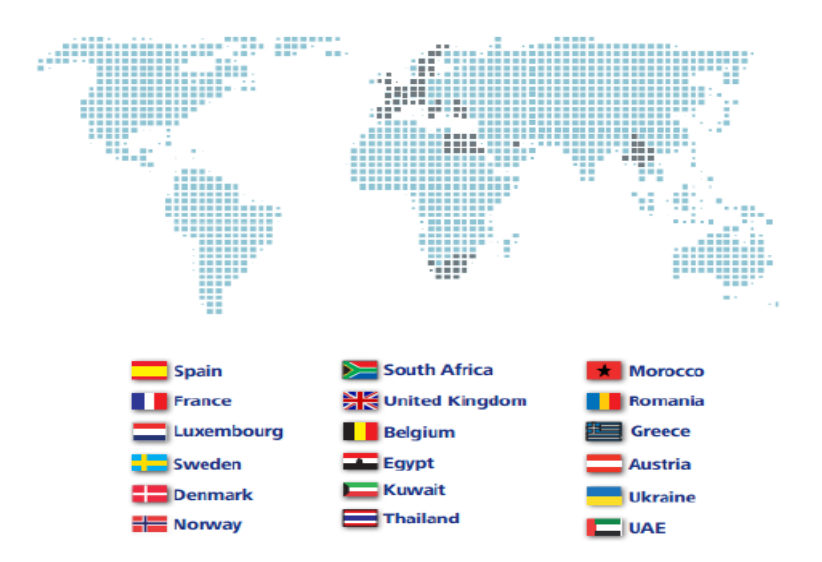
\includegraphics[width=0.9\columnwidth]{LesclientsdeVermegdanslemonde.png}}
        \caption{Les clients de Vermeg dans le monde }
        \label{fig:logo_tt}
    \end{figure}
\pagebreak
\subsection{Départements de Vermeg }
Les principaux départements  de Vermeg sont: \cite[]{vermeg}
\begin{itemize}
    \item \textbf{Recherche et Développement:} Se concentre sur l'innovation et le développement de nouvelles technologies et solutions.
    \item \textbf{Technologie et Développement de Produits :} Responsable de la conception, du  développement et de la maintenance des produits logiciels.
    \item \textbf{Ventes et Marketing :} Chargé de la promotion des produits et des services, de la gestion des relations clients et de l'acquisition de nouveaux clients.
    \item \textbf{Support Client et Services Professionnels :} Offre une assistance technique et des services de consultation aux clients.
    \item \textbf{Ressources Humaines :} Gère le recrutement, la formation, et le développement des employés ainsi que les relations de travail.
    \item \textbf{Finance et Comptabilité :} Gère les finances de l'entreprise, y compris la comptabilité, la gestion des budgets et les rapports financiers.
    \item \textbf{Gestion de Projet :} Assure la planification, l'exécution et la clôture des projets en respectant les délais et les budgets.
    \item \textbf{Qualité et Conformité :} Veille à ce que les produits et services répondent aux normes de qualité et aux réglementations en vigueur.
\end{itemize} 
Ces départements collaborent pour fournir des solutions technologiques complètes et innovantes aux clients de Vermeg dans les secteurs financiers et d'assurance. \\ 
Notre stage s'est effectué au sein du département Recherche et Développement.
\subsection{Services }
     L'activité de Vermeg s'articule principalement autour de quatre axes : \cite[]{vermeg}
    \begin{itemize}
        \item Assurance : couverture d’assurance individuelle ou de groupe pour l’épargne et la santé.
        \item Gestion de richesses et d’actifs : gestion des décisions financières dédiée aux besoins spécifiques de gestion du patrimoine.
        \item Marché financier et services de sécurité.
        \item Services financiers digitaux : numérisation des processus financiers et analyse des données sensibles.
    \end{itemize} 
    \pagebreak

    Vermeg fournit à ses clients un ensemble de logiciels spécialisés dans le domaine financier tels que :
    \begin{itemize}
        \item MEGARA (Securities processing) : La suite MEGARA est une plateforme modulaire pour le traitement des titres destinée essentiellement aux institutions financières qui propose un nombre de modules pouvant être implémentés séparément.
        \item PALMYRA : est un framework JEE compatible SOA (architecture orientée service) qui incorpore des composants ainsi que des services web réutilisables. L’implémentation de services web réutilisables permettant de développer des logiciels de meilleure qualité en temps réduit dont l’architecture est basée sur un client léger.
        \item SOLIFE : Une solution d’administration de polices d’assurance vie et un portail web à destination des clients finaux/brokers.
        \item SOLIAM : est une solution de gestion de portefeuilles pour les gestionnaires d’actifs institutionnels de fortune. Ayant une présence internationale en Belgique, France, Irlande, Luxembourg, Pays-Bas, Suisse, Royaume-Uni, Tunisie et des clients dans plus de 23 pays, VermegLife et Soliam sont considérés comme les deux produits phares de Vermeg BSB.
    \end{itemize} 
    
Maintenant que nous avons exploré la structure, les départements et les services de l'entreprise d'acceuil, et étant donné que Vermeg développe de nombreuses API et que notre projet s'inscrit dans ce contexte, nous allons aborder les concepts clés liés aux API.   

\section{Concepts clés autour des API}
Les API sont devenues des éléments essentiels du développement web moderne, permettant aux applications de communiquer et de partager des données. C’est pourquoi cette partie s'attache à présenter les fondements des API, leur documentation ainsi que le concept d'une marketplace d'API.
\subsection{Les Fondements des API }

    \subsubsection{Définition d'une API }
    Une API (Application Programming Interface) permet de rendre disponibles les données ou les fonctionnalités d’une application existante afin que d’autres applications les utilisent. Elle facilite le partage et l’intégration de fonctionnalités dans des architectures existantes. En pratique, une API agit comme un pont d'accès vers une fonction spécifique gérée par une entité distincte. \cite[]{DefAPI}
\pagebreak  
    \subsubsection{Fonctionnement d'une API }
    Une API fonctionne généralement selon le principe requête-réponse : 
    \begin{itemize}
        \item Requête: Le client envoie une requête à l'API, en précisant l'action souhaitée et les données nécessaires. 
        \item Réponse: L'API traite la requête et envoie une réponse au client, contenant les données ou les résultats de l'action demandée.
    \end{itemize} 

    \subsubsection{Types d'API}
    Les interfaces de programmation d’applications ne sont pas toutes créées de la même manière. Chaque type d’API a une utilité spécifique et s’intègre de manière différente dans l’écosystème des applications et des services. Voici les principaux types d'API selon les styles d’architecture : \\
    \textbf{a. API REST (Representational State Transfer) } \\
    Une API Rest est caractérisée par \cite[]{APIRest}:
    \begin{itemize}
        \item Architecture client-serveur sans état
        \item Accès aux ressources via des URL et des méthodes HTTP (GET, POST, PUT, DELETE)
        \item Formats de données courants : JSON, XML
        \item Facile à utiliser et à comprendre
        \item Flexible et évolutive  
    \end{itemize} 
    
    \textbf{b. API SOAP (Simple Object Access Protocol)  } \\
    Une API SOAP est caractérisée par \cite[]{APISOAP}:
    \begin{itemize}
        \item 	Architecture orientée service basée sur XML
        \item Utilisation de messages structurés et de protocoles web
        \item Norme plus complexe et plus lourde que REST
        \item Adaptée aux applications d'entreprise nécessitant une sécurité et une fiabilité élevées   
    \end{itemize} 

    \textbf{c. API RPC (Remote Procedure Call):} \\
    Une API RPC est caractérisée par  \cite[]{APIRPCGraphql}:
    \begin{itemize}
        \item Exécution des fonctions à distance sur un autre serveur
        \item Utilisation des protocoles spécifiques comme XML-RPC ou JSON-RPC
        \item Moins répandue que REST et SOAP, mais utile pour certaines applications telles que les systèmes distribués, les microservices, et les environnements nécessitant des appels de procédure rapides et directs  
    \end{itemize} 

    \textbf{d. API GraphQL } \\
    Une API graphQL est caractérisée par \cite[]{APIRPCGraphql}:
    \begin{itemize}
        \item Requêtes basées sur un schéma flexible
        \item Permet de récupérer des données précises et structurées
        \item Plus récent et plus moderne que REST et SOAP
        \item 	A Gagné en popularité pour son efficacité et sa flexibilité  
    \end{itemize} 

    \subsubsection{Structure d'une API}
    La structure d'une API comprend plusieurs éléments essentiels qui facilitent la communication entre le client et le serveur. Voici les composants :

    \begin{itemize}
        \item  \textbf{Endpoint : } C'est l'URL à laquelle l'API peut être accédée. Chaque endpoint correspond à une fonction spécifique de l'API. Par exemple, https://api.example.com/users peut être un endpoint pour accéder aux utilisateurs.
        \item \textbf{Méthodes HTTP : } Les actions possibles sur les ressources sont définies par les méthodes HTTP. Les plus courantes sont : GET, POST, PUT, DELETE
        \item  \textbf{En-têtes (Headers) : }  Informations supplémentaires envoyées avec les requêtes et les réponses HTTP, souvent utilisées pour l'authentification, la gestion du cache, le contrôle des formats de données, etc.
        \item \textbf{ Paramètres :}
        \begin{itemize}
            \item    \textbf{Path Parameters} Inclus dans l'URL pour spécifier une ressource particulière, par exemple, /users/{id}.
            \item \textbf{Query Parameters :} Inclus dans l'URL après le symbole \texttt{?} pour filtrer ou modifier la requête, par exemple, \texttt{?sort=asc\&limit=10}.
            \item  \textbf{Body Parameters}  Paramètres de corps (Body Parameters) : Utilisés principalement avec POST et PUT pour envoyer des données au serveur dans le corps de la requête.
        \end{itemize}
        \item  \textbf{Réponses:} Responses: Les réponses d'une API incluent le code de statut HTTP (par exemple, 200 pour le succès, 404 pour non trouvé, 500 pour une erreur serveur) et le corps de la réponse contenant les données ou les messages d'erreur
    \end{itemize} 
    
    
    Maintenant que nous avons examiné les fondements et les types d'API, il est essentiel de comprendre l'importance de la documentation qui est un élément crucial pour garantir la bonne utilisation et intégration d'une API.

    \subsection{Documentation d'une API }
    La documentation d'une API fournit aux développeurs et aux utilisateurs les clés pour exploiter pleinement le potentiel d'une API. En détaillant les endpoints, les méthodes, les paramètres, les réponses, les processus d'authentification, les exemples d'utilisation et la gestion des erreurs, elle éclaire les fonctionnalités de l'API et facilite son adoption.
    \subsubsection{Choix de la documentation  }
    Dans le domaine de la documentation des API, plusieurs formats sont utilisés, tels que Swagger/ OpenAPI, RAML, API Blueprint . Cependant, Swagger/OpenAPI est, en effet, l'un des formats les plus courants et les plus populaires.
    \subsubsection{Swagger/OpenAPI }

    Swagger a débuté comme un ensemble d'outils open-source développés par SmartBear Software pour simplifier la conception et la documentation des API RESTful. Avec le temps, il s'est transformé en un ensemble de spécifications et de formats permettant de décrire les API de manière claire et cohérente. En 2015, SmartBear Software a cédé la spécification Swagger à la fondation OpenAPI Initiative, qui l'a renommée OpenAPI Specification (OAS).
    Cette transition a élevé OpenAPI au rang de norme de l'industrie pour la documentation des API, offrant un standard largement adopté pour décrire les API de manière précise et uniforme. \cite[]{Swagger}

    \subsubsection{Caractéristiques d'un fichier Swagger/OpenAPI  }
    OpenAPI est une spécification de description d'API ouverte et standardisée. Elle permet de décrire les fonctionnalités d'une API de manière détaillée, notamment les endpoints, les paramètres, les réponses, etc… \\
    OpenAPI fournit un format standardisé pour la documentation des API. Les développeurs utilisent des fichiers au format JSON ou YAML pour décrire les API de manière claire et compréhensible.\cite[]{Swagger} \\
   La figure suivante présente un extrait d'un fichier swagger.
    \begin{figure}[H]    
    \centering
        \frame{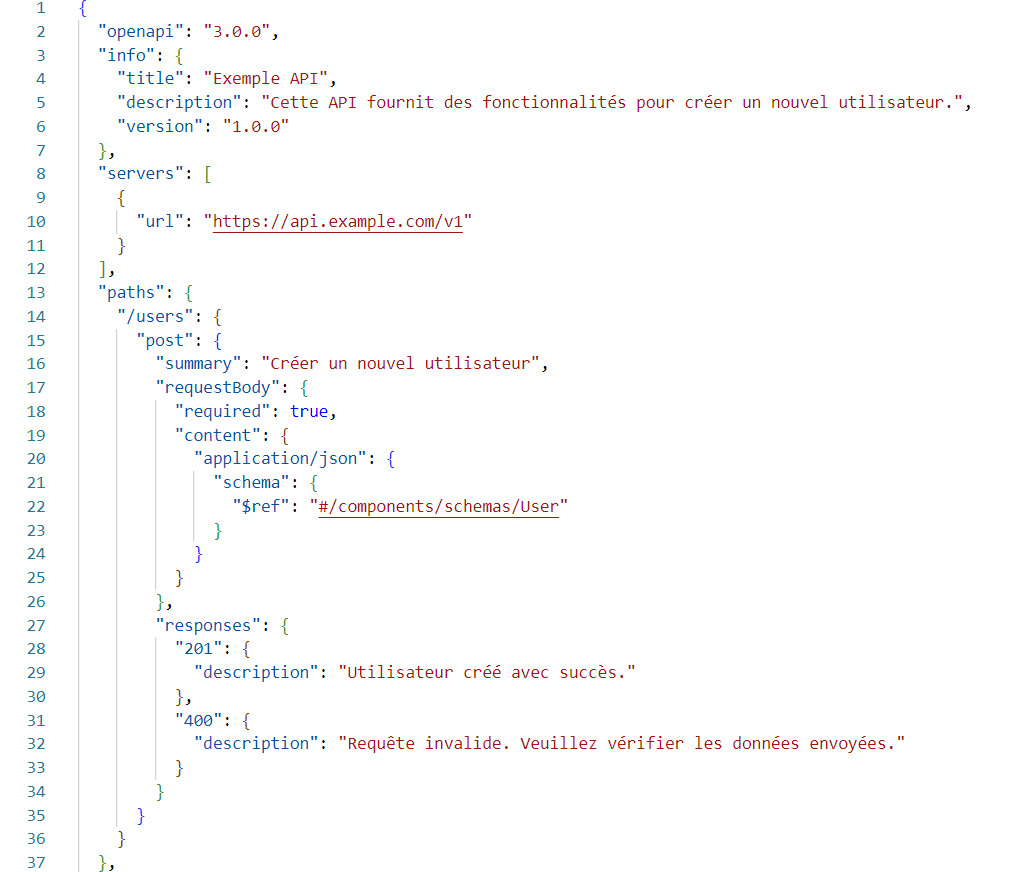
\includegraphics[width=1\columnwidth]{exemplefichierswagger.png}}
        \caption{Exemple de fichier swagger }
        \label{fig:logo_tt}
    \end{figure}
    Ce fichier Swagger décrit une API qui permet de créer un nouvel utilisateur via la méthode POST. 
    Lorsqu'un utilisateur est créé avec succès, la réponse sera un code 201 avec un message indiquant le succès de l'opération. 
    En cas de requête invalide, la réponse sera un code 400 avec un message informant l'utilisateur de vérifier les données envoyées. 
    \subsubsection{Avantages de Swagger/OpenAPI} 
        OpenAPI offre une documentation claire et cohérente pour les API, favorisant ainsi l'assimilation et l'adoption grâce à une documentation bien structurée. De plus, en adoptant OpenAPI, les organisations contribuent à la standardisation et à l'interopérabilité des API, simplifiant ainsi leur intégration avec différentes applications et systèmes. \\
        Bien que d'autres standards de documentation d'API, tels que RAML et API Blueprint, existent, Swagger et OpenAPI sont généralement préférés dans l'industrie en raison de leur large adoption, de leur écosystème d'outils et d'intégrations riches, ainsi que de leur soutien actif de la communauté.\cite[]{AvantageSwagger} 

    \subsubsection{Les outils de Swagger/OpenAPI }
    Plusieurs outils sont utilisés dans l'écosystème Swagger, tels que Swagger UI, Swagger Codegen et Swagger Editor. Swagger UI est utilisé pour afficher une interface interactive permettant aux développeurs et aux utilisateurs d'explorer facilement les endpoints, les paramètres et les réponses de l'API, améliorant ainsi la compréhension de son fonctionnement et favorisant son adoption.\cite[]{Swagger}
   
    \begin{figure}[H]    
        \centering
            \frame{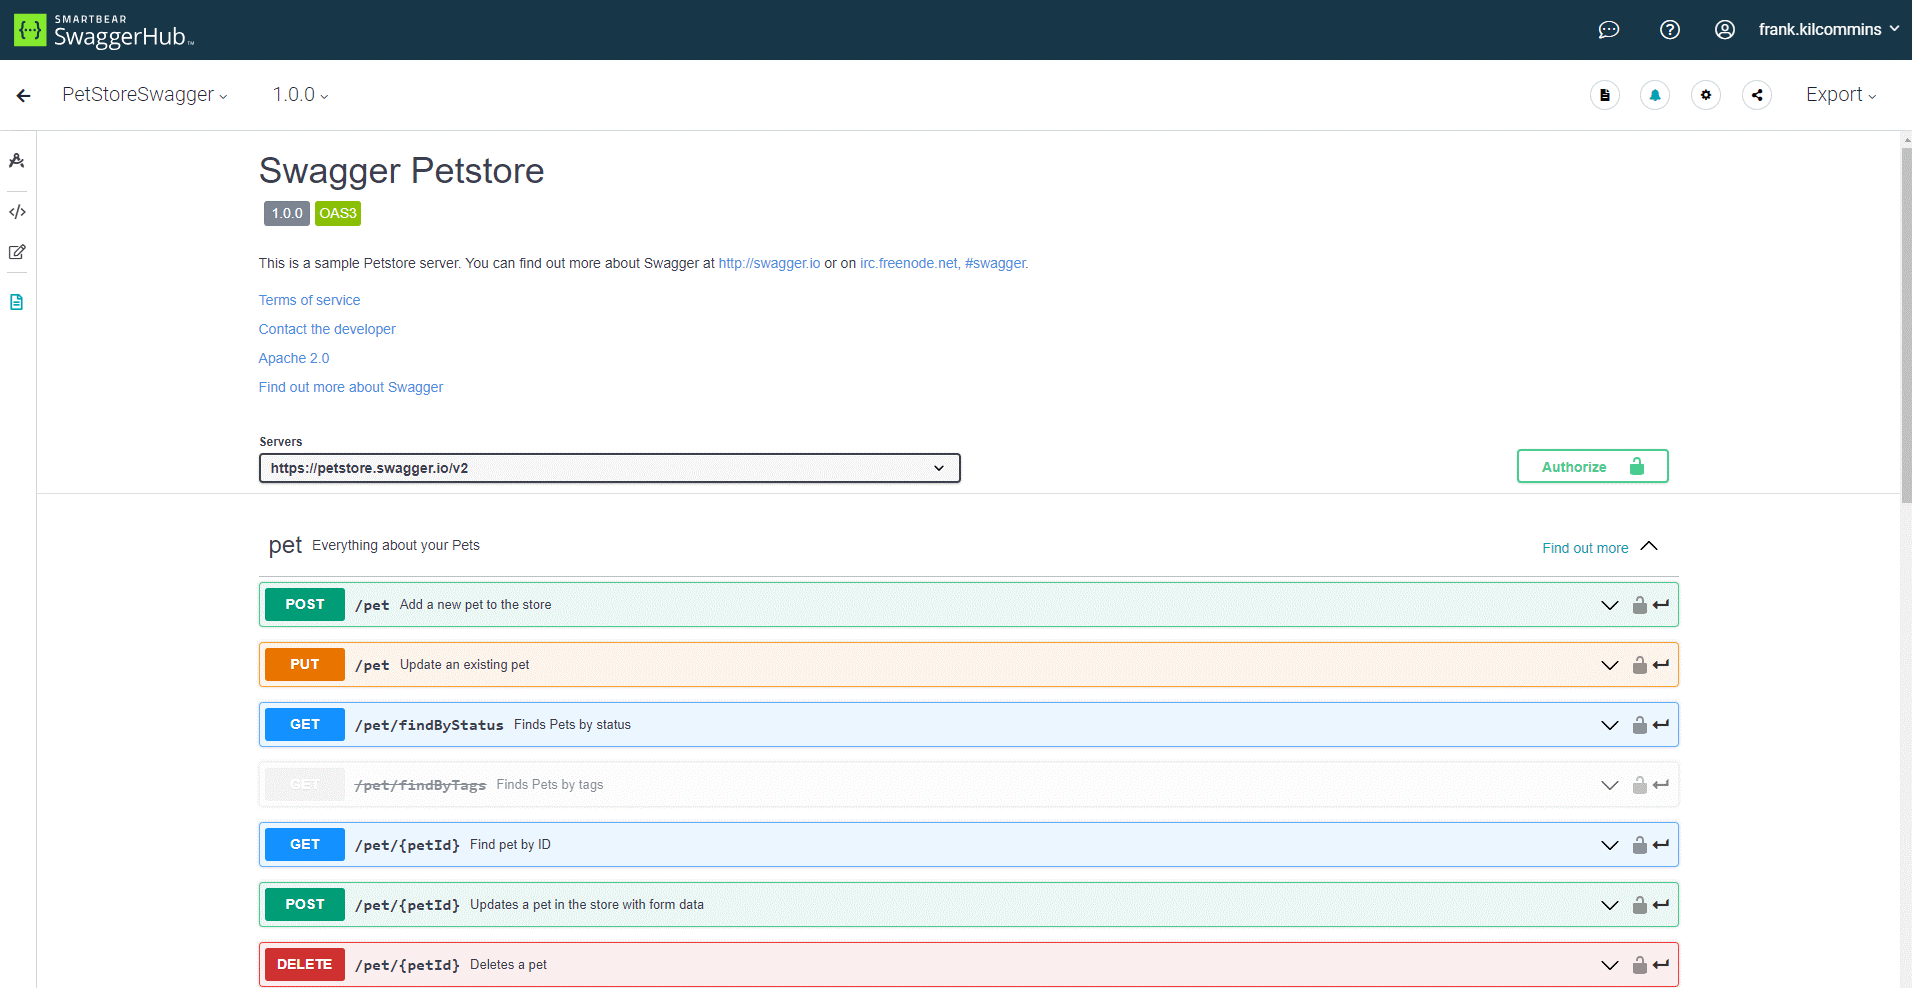
\includegraphics[width=1\columnwidth]{InterfacedeSwaggerUI.png}}
            \caption{Interface de Swagger UI }
            \label{fig:logo_tt}
        \end{figure}

       % Après avoir exploré la documentation détaillée des API, il est important de mentionner que Vermeg dispose de nombreuses API qui ne sont pas encore partagées ou pleinement utilisées. C'est pourquoi nous avons eu l'idée de créer un marketplace d'API où ces API peuvent être commercialisées et utilisées. Passons maintenant à l'exploration du concept de marketplace d'API, un espace dédié à la découverte, à l'échange et à la monétisation de ces API essentielles pour répondre aux besoins variés des développeurs et des entreprises.

       La documentation détaillée des API est cruciale pour leur adoption et leur utilisation efficace. Elle fournit une compréhension claire des fonctionnalités et des usages des API, facilitant leur intégration dans divers projets de développement. Cependant, la documentation seule ne suffit pas toujours à rendre les API largement accessibles. C'est ici qu'intervient le concept de marketplace d'API, qui offre un espace centralisé où les développeurs peuvent non seulement trouver et utiliser des API, mais aussi les commercialiser et les monétiser publiquement, rendant ainsi les API plus accessibles et favorisant une adoption plus large.

\pagebreak

\subsection{ MarketPlace d'API }

    \subsubsection{ Définition d'une marketPlace d’API} 


    Une marketplace d'API est une plateforme en ligne dédiée aux développeurs et aux entreprises pour découvrir, acheter, vendre et intégrer des API. \\
        Elle facilite l'échange de services et de données entre différents systèmes en offrant une plateforme centralisée pour les API, permettant ainsi aux fournisseurs de monétiser leurs API et aux consommateurs de trouver facilement les solutions dont ils ont besoin comme l’illustre la figure suivante:
        \begin{figure}[H]    
            \centering
                \frame{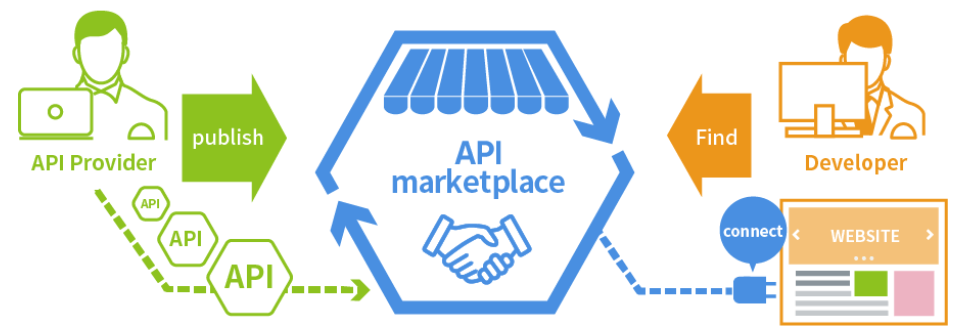
\includegraphics[width=0.8\columnwidth]{ProcessusdemarketplacedAPI.png}}
                \caption{ Fonctionnement d’une marketplace d’API \cite[]{marketplaceAPI} }
                \label{fig:logo_tt}
        \end{figure}
    \subsubsection{ Fonctionnalités d'une marketPlace d’API}

    Les fonctionnalités d'une API Marketplace varient d'une plateforme à l'autre, mais les plus courantes incluent :	
    \begin{itemize}
        \item    \textbf{Recherche d'APIs :}  Les développeurs d'applications peuvent rechercher des APIs par nom, par catégorie, par fonctionnalité, etc.
        \item  \textbf{Consultation des détails des APIs : }Les développeurs d'applications peuvent consulter les détails d'une API, tels que sa documentation, ses exemples de code, ses tarifs, etc.
        \item \textbf{Abonnement aux APIs : }Les développeurs d'applications peuvent s'abonner aux APIs qu'ils souhaitent utiliser.
        \item \textbf{Consommation des APIs :} Les développeurs d'applications peuvent utiliser les APIs auxquelles ils sont abonnés pour ajouter des fonctionnalités à leurs applications.
        \item  \textbf{Gestion des APIs :} Les fournisseurs d'API peuvent gérer leurs APIs sur la plateforme, en modifiant leurs informations, en ajoutant de nouvelles fonctionnalités et endpoints, etc.
    \end{itemize}
\pagebreak

    \subsubsection{ Avantages d'une marketPlace d’API}
Les API Marketplaces offrent plusieurs avantages tant pour les fournisseurs d'API que pour les développeurs d'applications : \\
\textbf{Pour les Fournisseurs d'API :} 
\begin{itemize}
    \item Augmentation de la visibilité de leurs APIs, ce qui peut conduire à une plus grande adoption et utilisation.
    \item Accès à un large bassin de développeurs d'applications intéressés par l'intégration de nouvelles fonctionnalités.
    \item Possibilité de générer des revenus grâce à la vente des APIs proposées sur la plateforme.
\end{itemize}
\textbf{Pour les consommateurs d'API :} 
\begin{itemize}
    \item Facilité à trouver et à intégrer les APIs nécessaires à leurs projets, grâce à une offre diversifiée et bien référencée.
    \item Économie de temps et d'argent en utilisant des APIs déjà existantes, évitant ainsi le développement de fonctionnalités complexes.
    \item Ajout de nouvelles fonctionnalités à leurs applications sans nécessiter un développement \\ supplémentaire, grâce à la disponibilité d'API prêtes à l'emploi.
    \item L'intégration de ces avantages dans une API Marketplace favorise la collaboration et l'innovation dans l'écosystème des développeurs d'applications.
\end{itemize}

\subsection{Acteurs du domaine métier}
Les principaux acteurs du domaine métier des marketplaces d'API sont les suivants :
\begin{itemize}
    \item    \textbf{Fournisseurs d'API :}  Les fournisseurs d'API sont les entreprises ou les organisations qui développent et publient des APIs.
    \item  \textbf{Consommateur d’API :} Les développeurs d'applications sont les utilisateurs qui utilisent les APIs pour ajouter des fonctionnalités à leurs applications.
    \item \textbf{Plateformes des marketplaces d'API:} Les plateformes des marketplaces d'API sont les plateformes en ligne qui mettent en relation les fournisseurs d'API et les développeurs d'applications.
\end{itemize}
        \pagebreak

\section{Etude de marché}
Cette étude constitue une partie importante de la phase d’analyse d’un projet qui pourra nous orienter pour tirer des avantages de ces solutions et remédier à leurs inconvénients. Cette étape est primordiale pour la mise en route de tout projet informatique.  Parmi les marketplaces existantes, voici une comparaison de certaines d'entre elles : RapidAPI, API Layer, OpenAPIHub et Zyla Labs. \cite[]{site1} \cite[]{site2}


\captionsetup[table]{justification=centering}

\begin{longtable}[c]{
    |>{\centering\arraybackslash}p{.15\textwidth}
    |>{\centering\arraybackslash}p{.20\textwidth}
    |>{\centering\arraybackslash}p{.20\textwidth}
    |>{\centering\arraybackslash}p{.20\textwidth}
    |>{\centering\arraybackslash}p{.20\textwidth}|
    }
\caption{Etude comparative des principales marketplaces d’API}
\label{tab:comparaison_fournisseurs_api}                                                                                                                                                                                                                                                                                                                                                                                                                         \\
\hline
\textbf{Critère} & \textbf{RapidAPI} & \textbf{API Layer} & \textbf{OpenApiHub} & \textbf{Zyla Labs}                                                                                             \\
\hline
\endfirsthead
\hline
\endhead
\hline
\endfoot
\hline
\endlastfoot

Intermédiaire \footnote{désigne le rôle de la plateforme qui gère toutes les transactions, requêtes et crédits entre les fournisseurs et les utilisateurs d'API, assurant que toutes les interactions passent par elle et non directement par le fournisseur de services d'API.} & Oui & Oui & Oui & Oui \\
\hline
Documentation sur les API & Oui & Oui & Oui & Oui \\
\hline
Définition des endpoints & Manuellement  \hspace{1cm}(un à un) & À travers la documentation Swagger & À travers la documentation Swagger & Manuellement \hspace{1cm} (un à un)  \\
\hline
Test d'exemple sur la plateforme  & Oui & Oui & Oui & Oui \\
\hline
Mesure de la latence de l’ API  & Oui & Non & Oui & Oui \\
\hline
Mise à niveau d’un plan de tarification & Ancien crédit perdu & Ancien crédit perdu & Ancien crédit perdu & Montant déduit Selon Requêtes non utilisés \\
\hline
Ajout d'un plan de tarification & Non flexible & Non flexible & Non flexible & Non flexible \\
\hline
Tarification pour les consommateurs d'API  \footnote{Les utilisateurs ont la possibilité de choisir entre un plan gratuit et un plan payant basé sur le nombre de requêtes effectuées pendant une période définie.} & Gratuit, Payant par nombre de requêtes pendant une durée précise & Gratuit, Payant par nombre de requêtes pendant un mois & Gratuit, Payant par nombre de requêtes pendant un mois & Gratuit, Payant par nombre de requêtes pendant un mois ou par an \\
\hline
Frais de la plateforme (Commission)  & 20\% & 15\% & Gratuit (20\%), Essential (12\%), Professional (8\%), Business, Enterprise & 10\% \\
\hline
Signalement d'erreurs & Non & Oui & Non & Non  \\
\hline
Notifications & Oui, mais pas en temps réel & Non & Non & Non \\
\hline
Mode de paiement & Stripe & Stripe & Stripe & Stripe \\
\hline
\end{longtable}


Cette étude comparative a démontré que:
\begin{itemize}
    \item \begin{minipage}[t]{\linewidth}
        Toutes ces marketplaces jouent le rôle d’intermédiaire, fournissent une documentation et permettent de tester un exemple.
      \end{minipage}
      \vspace{1pt}

    \item Pour l’ajout d’endpoints, RapidAPI et Zyla Labs nécessitent une intervention manuelle (au risque de commettre des erreurs), tandis qu’API Layer et OpenApiHub utilisent la documentation standardisée de Swagger pour simplifier ce processus
    
    \item Seules RapidAPI, OpenApiHub et Zyla Labs fournissent des mesures de latence des API.
    \item Lors de la mise à niveau d’un plan de tarification, l’utilisateur perd ses crédits non utilisés avec RapidAPI, API Layer et OpenApiHub alors qu’il bénéficie d’une réduction avec la marketplace Zyla Labs.
    \item RapidAPI, API Layer, OpenApiHub et Zyla Labs proposent des plans de tarification qui manquent de flexibilité dans la définition des termes du plan de tarification. 
    \item Les commissions prélevées par les plateformes varient entre 8 \% et 20 \%.
    \item Le signalement d'erreurs, tel qu'en cas de bug, est une fonctionnalité offerte uniquement par API Layer.
    \item RapidAPI est la seule plateforme à proposer des notifications , bien qu'elles ne soient pas en temps réel.
    \item Toutes les plateformes utilisent Stripe comme mode de paiement, assurant ainsi une solution sécurisée et reconnue.
\end{itemize}
\pagebreak
\section{Description et critique de l’existant}

\subsection{Description et critique de l'existant }
Actuellement, au sein de Vermeg, le département de recherche et développement se focalise sur la création d’APIs internes, incluant des modèles de machine learning. Cependant, ces APIs ne sont pas accessibles à la communauté des développeurs, limitant le potentiel de l’entreprise à générer des revenus supplémentaires et à accroître sa visibilité. \\
Pour remédier à cela, Vermeg souhaite rendre ses APIs accessibles au public, introduisant ainsi un nouveau produit sur le marché. \\
Toutefois, Vermeg ne souhaite pas recourir à des solutions et plateformes existantes pour plusieurs raisons : 
\begin{itemize}
    \item Les solutions disponibles ne répondent pas parfaitement aux besoins spécifiques de l’entreprise en termes de sécurité et de personnalisation. 
    \item Les coûts d’utilisation de ces plateformes tierces peuvent être élevés, réduisant ainsi les marges bénéficiaires potentielles.
    \item Vermeg vise à maintenir un contrôle total sur la distribution et la monétisation de ses APIs, garantissant ainsi une flexibilité maximale et une adaptation précise aux besoins futurs. 
\end{itemize}

\subsection{Solution proposée}

Nous proposons de créer une marketplace d'API, nommée "InfinityAPI", qui permettra aux développeurs de publier et de monétiser leurs API sur la plateforme. Cette marketplace offrira un espace centralisé où les développeurs pourront consulter, souscrire et consommer des API, avec également la possibilité de fournir des API à des fins commerciales.

InfinityAPI doit être conçue en tenant compte de l'étude de marché sur les marketplaces existantes. Pour être compétitive, la plateforme devrait offrir :
\begin{itemize}
    \item Une intégration simplifiée des API grâce à l'utilisation de fichiers Swagger.
    \item Une tarification flexible en termes de nom, de prix et de nombre de requêtes.
    \item La possibilité de mettre à niveau les plans sans perte de crédits.
    \item Une commission modérée en fonction des fonctionnalités proposées.
    \item Un paiement sécurisé avec Stripe.
    \item Des notifications en temps réel.
\end{itemize}
En adoptant cette approche, Vermeg et d’autres fournisseurs d’API pourront non seulement rentabiliser leurs investissements dans le développement d’API, mais aussi générer des revenus supplémentaires.


\section{Méthodologie adoptée et langage de modélisation}
Il existe plusieurs méthodologies de développement, chacune ayant ses propres avantages et inconvénients. Le choix de la bonne méthode dépend des exigences du projet, de la taille de l'équipe, des objectifs, des ressources disponibles et du calendrier.

\subsection{Choix de la méthodologie  } 

Pour notre projet de fin d'études "InfinityAPI", il est crucial d'adopter une méthodologie de développement qui permette de: 
\begin{itemize}
    \item S'adapter rapidement aux exigences du client.
    \item Livrer régulièrement les fonctionnalités prioritaires 
    \item  Favoriser une collaboration étroite entre les membres d'équipe .
\end{itemize}
Afin de répondre à ces besoins, nous avons opté pour l’approche agile à travers le framework Scrum.

Scrum permet de développer notre solution de manière itérative et incrémentale, en se concentrant sur des cycles de développement courts appelés sprints. Cette approche garantit une livraison régulière de fonctionnalités à forte valeur ajoutée et offre la flexibilité nécessaire pour ajuster notre travail en fonction des changements de priorités et des besoins du product owner.

En adoptant Scrum, nous assurons une communication continue et une meilleure collaboration en équipe, tout en maintenant une qualité élevée du produit final. \cite[]{Scrum}\\ 
Le processus de scrum est illustré dans la figure suivante:
%Pour notre projet de "Infinity API", il est impératif d'adopter une approche de développement qui permette une adaptation rapide aux exigences du product owner, une livraison efficace des fonctionnalités prioritaires, ainsi qu'une collaboration étroite et efficace avec l'équipe de développement. \\Afin de répondre à ces exigences, nous avons choisi d'implémenter une méthodologie Agile pour notre projet.L'Agilité nous permet de développer notre solution de manière itérative, en nous concentrant sur la livraison régulière de fonctionnalités à forte valeur ajoutée. Plus particulièrement, nous avons opté pour Scrum, une méthodologie Agile bien établie. \\Scrum nous offre la structure nécessaire pour organiser notre travail en sprints, des cycles de développement courts et itératifs. Cette approche nous permet de prioriser les fonctionnalités les plus importantes à chaque itération, tout en restant flexibles pour nous adapter aux changements de priorités et de besoins du product owner. \\En optant pour Scrum, nous sommes confiants dans notre capacité à livrer un produit de haute qualité qui répondra aux attentes du product owner. Cette approche nous offre une flexibilité accrue, nous permettant d'ajuster rapidement notre travail en fonction des besoins changeants. Les sprints réguliers garantissent des livraisons fréquentes de fonctionnalités, favorisant ainsi une meilleure collaboration au sein de l'équipe. \\En résumé, l'adoption de l'approche Agile, notamment Scrum, représente la solution optimale pour notre projet de "marketplace d'API". Elle nous permet de répondre efficacement aux besoins évolutifs du marché tout en assurant la satisfaction du product owner et des utilisateurs finaux.
\begin{figure}[H]    
    \centering
        \frame{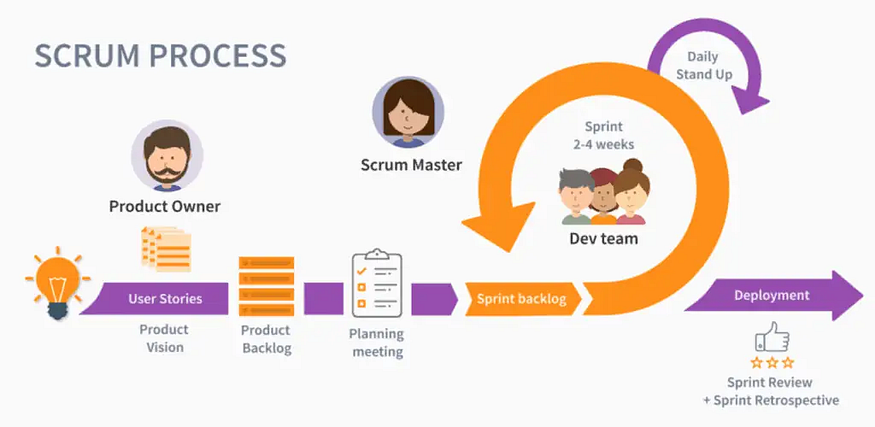
\includegraphics[width=0.8\columnwidth]{Processusde scrum.png}}
        \caption{Processus de Scrum}
        \label{fig:logo_tt}
    \end{figure}

\subsection{Langage de modélisation}

Le Unified Modeling Language (UML) a été conçu pour être un langage de modélisation visuel. Il est prévu pour l'architecture, la conception et l'implémentation de systèmes logiciels complexes par leur structure ainsi que leur  comportement. UML dispose d'applications qui vont au-delà du développement logiciel, en particulier pour les flux de processus dans l'industrie. Il ressemble aux plans utilisés dans d'autres domaines et se compose de différents types de diagrammes. D'une façon générale, les diagrammes UML décrivent les frontières, la structure et le comportement du système et de ses objets. \cite[]{UML}

\section*{Conclusion}

Dans cette section, nous avons introduit « Vermeg », notre organisme d’accueil. Ensuite, nous avons examiné les concepts clés liés aux API, réalisé une étude de marché, une étude de l’existant et enfin, argumenté du choix de la méthodologie de développement et du langage de modélisation .Dans le deuxième chapitre, nous aborderons la planification du projet. 



        \clearpage
        
        \chapter{Planification du projet}

\section*{Introduction}
Ce chapitre commence par la spécification des besoins, en présentant les besoins fonctionnels et non fonctionnels. Ensuite, il aborde la gestion du projet avec Scrum, en présentant l'équipe Scrum, le backlog du produit et la planification de la release. Enfin, nous examinons l'environnement de développement, l'architecture et les patrons de conception adaptés.

\section{Spécification des besoins}

Notre projet vise à développer une plateforme de marketplace d'API « Infinity API », permettant aux développeurs et aux entreprises d'intégrer et de consommer facilement des API de manière simplifiée. //
Afin d'atteindre cet objectif, nous exposons les exigences fonctionnelles et non fonctionnelles de notre plateforme.

    \subsection{Les besoins fonctionnels } 
    Les besoins fonctionnels de notre projet se résument comme suit :
    \begin{itemize}
        \item  \textbf{Gestion des API}
        \begin{itemize}
            \item Ajout d’une API avec la documentation Swagger, qui regroupe ainsi les endpoints, les descriptions des requêtes et des réponses.
            \item Consultation, modification et suppression d'une API par un développeur. 
        \end{itemize}
        \item \textbf{Gestion de la tarification des API}
        \begin{itemize}
            \item Création, modification et suppression de plans de tarification pour une API. Un plan de tarification est composé du nom du plan, du nombre de requêtes, de la durée et du prix.
            \item Consultation des plans de tarification disponibles pour une API. 
        \end{itemize}
        \item \textbf{Catalogue d’API}
        \begin{itemize}
            \item Consultation de la liste des API par un utilisateur. 
            \item Filtrage des APIs selon différents critères. 
            \item Consultation des détails de chaque API. 
        \end{itemize}
        \item \textbf{Gestion de la souscription à une API}
        \begin{itemize}
            \item Souscription à une API après avoir choisi le plan de tarification qui convient pour un plan de tarification payant, la souscription engendre une opération de paiement. 
            \item Consultation de la liste des souscriptions.  
            \item Annulation d’une souscription. 
            \item Consultation de l'historique des souscriptions.
            \item Mise à niveau de la souscription pour obtenir un quota de requêtes plus élevé et une durée de validité étendue.
            \item Consultation de l'historique des payements.
        \end{itemize}
        \item \textbf{Consommation et test des API}
        \begin{itemize}
            \item Consommation d’une API, qui consiste à utiliser les endpoints pour effectuer des requêtes et récupérer les données nécessaires.
            \item Test des API et leur consommation sur la plateforme « Infinity API ».          
        \end{itemize}
        \item \textbf{Gestion des transactions}
        \begin{itemize}
            \item Consultation du montant disponible sur le compte d’un développeur gagner de la plateforme.
            \item Vérification des transactions effectuées sur l’API fournier par un développeur.
            \item Demande d’un prélèvement du solde disponible sur le compte.
            \item Gestion des demandes de prélèvement par l'administrateur.    
        \end{itemize}
        \item \textbf{Dashboard Administrateur}
        \begin{itemize}
            \item Consultation de la liste des développeurs inscrits sur la plateforme.
            \item Blocage et déblocage d’un compte développeur.   
        \end{itemize}
        \item \textbf{Gestion des catégories} \\
         Ajout, modification, suppression et consultation de catégories.
         \item \textbf{Gestion des comptes utilisateur }
         \begin{itemize}
             \item Inscription d'un nouveau développeur.
             \item Consultation, modification d’un profil utilisateur.   
             \item Suppression d'un profil développeur.
         \end{itemize}
         \item \textbf{Gestion des signalements de problèmes}
         \begin{itemize}
             \item Signalement d’un problème lié à une API.
             \item Consultation des signalements par l’administrateur et par le développeur qui a fourni l’API.  
         \end{itemize}
         \item \textbf{Gestion des feedbacks}
         \begin{itemize}
             \item Création, modification, et suppression d’un commentaire relatif à une API.
             \item Consultation des commentaires laissés par les développeurs. 
         \end{itemize}
         \item \textbf{Suivi et statistiques }
         \begin{itemize}
             \item Suivi des payements et des statistiques liées à l’utilisation de la plateforme.
             \item Suivi des statistiques de performance et d'état des APIs.
             \item Suivi des statistiques de paiement des APIs.
         \end{itemize}
         \item \textbf{Système de notification  } \\
         La marketplace doit fournir des notifications suite aux différentes opérations effectuées sur la plateforme.
    \end{itemize}        
    % Une deuxième sous section
    \subsection{Les besoins non fonctionnels }
    Les besoins non fonctionnels de notre projet se résument comme suit : 
    \begin{itemize}
        \item \textbf{Sécurité des données }
        \begin{itemize}
            \item Authentification des utilisateurs.
            \item o	Utilisation de mécanismes de sécurité pour protéger les données des utilisateurs.
        \end{itemize}
        \item \textbf{Ergonomie de l'interface }\\
        La navigation intuitive et claire entre les différentes interfaces de l'application.
        \item \textbf{Fiabilité  }\\
        Minimiser les erreurs de serveur pour garantir une expérience utilisateur stable et fiable.
        \item \textbf{Documentation des API avec Swagger  }\\
        Utilisation de Swagger pour créer une documentation détaillée des API ajoutées à la plateforme, facilitant ainsi l'intégration et l'utilisation par les développeurs tiers.
        \item \textbf{Intégration de services de paiement en ligne }\\
        Intégration de services comme Stripe et PayPal pour permettre des transactions sécurisées lors de la souscription aux plans de tarification payants et des prélèvements de solde.
    \end{itemize}        

% Une deuxième section Pilotage du projet avec Scrum 
\section{Pilotage du projet avec Scrum }
Dans cette partie, nous allons aborder la présentation de l'équipe Scrum ainsi que le backlog du produit et pour finir, la planification de la release.
    \subsection{Equipe et rôles  } 
    Avant de présenter le product backlog, il est important d'introduire l'équipe de travail :
    \begin{itemize}
        \item \textbf{Le Product Owner }:M.Akram ANAYA :Chef projet de l’équipe de développement 
        \item \textbf{Le Scrum Master }: M.Ahmed GHIZWENI : Chef de produit
        \item \textbf{Les développeurs  }: Yassine LASSOUED et Ayoub SHILI
    \end{itemize} 
    \subsection{Le backlog du produit  } 
    Nous avons utilisé une échelle basée sur la suite de Fibonacci. Les valeurs attribuées sont les suivantes  : 1 pour "Très facile", 2 pour "Facile", 3 pour "Assez simple", 5 pour "Moyen", 8 pour "Assez compliqué", 13 pour "Compliqué" et 20 pour "Très compliqué". Dans le cas de notre marketPlace ,les utilisateurs sont : \\
    \begin{itemize}
        \item \textbf{Visiteur }:c’est un internaute qui n'a pas encore été authentifié.
        \item \textbf{Développeur  }: qui est inscrit sur notre plateforme, il peut jouer le rôle de fournisseur ou de consommateur d’API
        \item \textbf{Administrateur }: qui gère la plateforme.
    \end{itemize} 

    \begin{longtable}[c]{
        |p{.10\textwidth}
        |p{.20\textwidth}
        |p{.10\textwidth}
        |p{.30\textwidth}
        |p{.10\textwidth}
        |p{.05\textwidth}
        |p{.05\textwidth}|
    }
        \caption{Tableau long}
        \label{tab:myfirstlongtable}\\
        \hline
        \textbf{US ID} & \textbf{Thème} & \textbf{En Tant que} & \textbf{User Story} & \textbf{Valeur Business} & \textbf{Effort} & \textbf{Priorité} \\
        \hline 
        \endfirsthead
        \multicolumn{7}{c}%
        {{\bfseries \tablename\ \thetable{} -- suite de la page précédente}} \\
        \hline 
        \textbf{US ID} & \textbf{Thème} & \textbf{En Tant que} & \textbf{User Story} & \textbf{Valeur Business} & \textbf{Effort} & \textbf{Priorité} \\
        \hline 
        \endhead
        \hline \multicolumn{7}{|r|}{{\bfseries Suite à la page suivante}} \\ \hline
        \endfoot
        \hline
        \endlastfoot
        
        1 & Création du compte Utilisateur & Visiteur & Je souhaite pouvoir m'inscrire pour créer un compte. & Haute & 5 & Haute \\
        \hline
        2 & Authentification & Développeur ou Administrateur & Je souhaite pouvoir m'authentifier pour accéder à mon compte. & Haute & 13 & Haute \\
        \hline
        3 & Gestion des catégories & Administrateur & Je veux créer une nouvelle catégorie en spécifiant son nom, sa description et d'autres informations pertinentes. & Haute & 2 & Haute \\
        \hline
        4 & & Administrateur & Je veux modifier les détails d'une catégorie existante. & Haute & 2 & Haute \\
        \hline
        5 & & Administrateur & Je veux supprimer une catégorie. & Haute & 1 & Haute \\
        \hline
        6 & & Administrateur & Je veux consulter la liste des catégories existantes sur la plateforme. & Haute & 2 & Haute \\
        \hline
        7 & Gestion des APIs & Développeur & Je veux pouvoir ajouter une nouvelle API pour fournir une API aux autres utilisateurs. & Haute & 20 & Haute \\
        \hline
        8 & & Développeur & Je veux consulter la liste de mes APIs pour visualiser rapidement toutes les APIs que j'ai créées. & Haute & 5 & Haute \\
        \hline
        9 & & Développeur & Je veux pouvoir modifier les informations de mon API pour mettre à jour les informations. & Haute & 5 & Haute \\
        \hline
        10 & & Développeur & Je veux pouvoir supprimer mon API car elle n'existe plus ou contient beaucoup de signalments d'erreurs. & Haute & 2 & Haute \\
        \hline
        11 & Consultation, filtrage et recherche sur les APIs & Utilisateur & Je veux pouvoir consulter la liste des APIs pour pouvoir chercher l’API qui répond à mes besoins. & Haute & 5 & Haute \\
        \hline
        12 & & Utilisateur & Je veux pouvoir consulter les détails d'une API pour découvrir ses fonctionnalités. & Haute & 8 & Haute \\
        \hline
        13 & & Utilisateur & Je veux pouvoir rechercher une API par son nom pour la trouver rapidement et facilement. & Haute & 2 & Haute \\
        \hline
        14 & & Utilisateur & Je veux pouvoir faire un filtrage avancé sur les APIs pour trouver celles qui correspondent le mieux à mes besoins. & Haute & 5 & Haute \\
        \hline
        15 & Gestion du compte Utilisateur & Développeur ou Administrateur & Je veux pouvoir consulter mon profil pour vérifier mes informations personnelles. & Haute & 3 & Haute \\
        \hline
        16 & & Développeur ou Administrateur & Je veux pouvoir modifier mon profil pour mettre à jour mes informations. & Haute & 5 & Haute \\
        \hline
        17 & & Développeur & Je veux pouvoir supprimer mon compte pour me désinscrire de la plateforme. & Haute & 2 & Haute \\
        \hline
        18 & Gestion de la tarification & Développeur & Je veux pouvoir créer des plans de tarification pour mon API pour proposer différents niveaux d'accès à mon API et générer des revenus. & Moyenne & 8 & Haute \\
        \hline
        19 & & Développeur & Je veux pouvoir consulter les plans de tarification pour suivre les options disponibles pour mes APIs. & Moyenne & 3 & Haute \\
        \hline
        20 & & Développeur & Je veux pouvoir modifier des plans de tarification pour mon API pour pouvoir mettre à jour les prix et les limites d'utilisation. & Moyenne & 5 & Haute \\
        \hline
        21 & & Développeur & Je veux pouvoir supprimer un plan de tarification pour mon API si la tarification n'est plus nécessaire. & Moyenne & 2 & Haute \\
        \hline
        22 & & Utilisateur & Je veux pouvoir consulter les plans de tarification pour une API afin de choisir celui qui correspond le mieux à mes besoins et à mon budget. & Moyenne & 3 & Haute \\
        \hline
        23 & Souscription & Développeur & Je veux pouvoir souscrire à une API pour accéder aux fonctionnalités qu'elle propose. & Moyenne & 20 & Haute \\
        \hline
        24 & & Développeur & Je veux pouvoir consulter la liste de mes souscriptions pour suivre mes souscriptions. & Moyenne & 2 & Haute \\
        \hline
        25 & & Développeur & Je veux pouvoir effectuer une mise à niveau de ma souscription d'API. & Moyenne & 8 & Haute \\
        \hline
        26 & & Développeur & Je veux pouvoir annuler une souscription. & Moyenne & 3 & Haute \\
        \hline
        27 & Consommation et test d'une API & Développeur & Je veux pouvoir consommer une API et l'intégrer dans mon projet afin d'utiliser ses fonctionnalités. & Moyenne & 13 & Haute \\
        \hline
        28 & & Développeur & Je veux pouvoir tester l'API sur la plateforme pour savoir si elle fonctionne correctement et qu'elle répond aux besoins des développeurs. & Moyenne & 20 & Haute \\
        \hline
        29 & Dashboard Administrateur & Administrateur & Je veux pouvoir consulter la liste des développeurs et suivre leurs activités. & Moyenne & 3 & Moyenne \\
        \hline
        30 & & Administrateur & Je veux pouvoir rechercher un utilisateur. & Moyenne & 2 & Moyenne \\
        \hline
        31 & & Administrateur & Je veux pouvoir consulter les détails d'un développeur pour comprendre son activité et ses interactions avec la plateforme. & Moyenne & 8 & Moyenne \\
        \hline
        32 & & Administrateur & Je veux pouvoir bloquer/débloquer un compte développeur pour contrôler tout comportement abusif ou non autorisé. & Moyenne & 3 & Moyenne \\
        \hline
        33 & Gestion des transactions & Développeur & Je veux pouvoir consulter le montant disponible sur mon compte afin de suivre mes revenus générés par la vente d'API sur la plateforme. & Moyenne & 3 & Moyenne \\
        \hline
        34 & & Développeur & Je veux pouvoir vérifier les transactions effectuées via mon API afin de tracer l'origine de mes revenus. & Moyenne & 3 & Moyenne \\
        \hline
        35 & & Développeur & Je veux pouvoir effectuer une demande de prélèvement du solde disponible sur le compte. & Moyenne & 8 & Moyenne \\
        \hline
        36 & & Administrateur & Je veux pouvoir gérer les demandes de prélèvement en les acceptant ou en les refusant. & Moyenne & 5 & Haute \\
        \hline
        37 & Dashboards de Statistiques & Développeur & Je veux pouvoir suivre les statistiques de performance de mon API pour surveiller son utilisation et sa qualité de service. & Faible & 13 & Moyenne \\
        \hline
        38 & & Développeur & Je veux pouvoir suivre les statistiques d'utilisation de mon API (nombre de requêtes, nombre de développeurs, etc.) pour suivre l'utilisation de mon API. & Faible & 20 & Moyenne \\
        \hline
        39 & & Administrateur & Je veux pouvoir suivre les statistiques de performance des API pour surveiller la qualité de service globale de la plateforme. & Faible & 13 & Moyenne \\
        \hline
        40 & & Administrateur & Je veux pouvoir suivre les statistiques des paiements sur la plateforme pour surveiller les revenus de la plateforme. & Faible & 13 & Moyenne \\
        \hline
        41 & Gestion des signalements & Développeur & Je veux pouvoir signaler un problème pour obtenir une assistance ou signaler des problèmes de fonctionnement. & Faible & 5 & Moyenne \\
        \hline
        42 & & Développeur & Je veux pouvoir consulter mes signalements d'erreurs. & Faible & 3 & Moyenne \\
        \hline
        43 & & Administrateur & Je veux pouvoir consulter les signalements d'erreur pour suivre les problèmes identifiés par les développeurs. & Faible & 3 & Faible \\
        \hline
        44 & Gérer les feedbacks & Développeur & Je veux pouvoir ajouter un commentaire à une API pour partager mon avis sur l'API. & Faible & 3 & Faible \\
        \hline
        45 & & Développeur & Je veux pouvoir consulter les commentaires laissés par les développeurs d'une API afin de connaître leur opinion sur celle-ci. & Faible & 2 & Faible \\
        \hline
        46 & & Développeur & Je veux pouvoir modifier mon commentaire si je souhaite les rectifier. & Faible & 2 & Faible \\
        \hline
        47 & & Développeur & Je veux pouvoir supprimer mon commentaire si je souhaite le retirer de la plateforme. & Faible & 2 & Faible \\
        \hline
        48 & Système de notification & Développeur ou Administrateur & Je veux pouvoir consulter les notifications. & Faible & 8 & Faible \\
        \hline
    
    \end{longtable}
    
\section{Identification des scénarios}

    
    
\section{Diagramme de GANTT théorique}
    
    
\section*{Conclusion}
    Conclusion partielle ayant pour objectif de synthétiser le chapitre et d’annoncer le chapitre suivant.
        \clearpage
        
        \chapter{Sprint 1 "La gestion des APIs et des catégories"}

\section*{Introduction}
Dans ce chapitre, nous abordons, en détail, le premier sprint de notre projet. Nous allons parcourir les différentes étapes de ce sprint, de la planification à la mise en œuvre, en mettant en exergue le backlog du sprint 1, la spécification fonctionnelle, la conception, la revue du sprint et pour finir  la rétrospective.

\section{Extrait du backlog du sprint 1}

    Les thèmes du premier sprint sont : l’authentification, la gestion des catégories, la gestion des API ainsi que le filtrage, la recherche d'API et la gestion des comptes utilisateurs. \\
    Nous allons maintenant présenter un extrait du backlog du sprint : “Ajouter une API” et nous allons détailler ce que nous prévoyons de faire pendant ce sprint; les tâches des autres user stories sont considérées comme étant similaires.

    \captionsetup[table]{justification=centering}

    \begin{longtable}[c]{|p{0.25\linewidth}|p{0.25\linewidth}|p{0.25\linewidth}|p{0.15\linewidth}|}
        \caption{Extrait du backlog du sprint 1 "Ajouter une API"} \\
        \hline
        \textbf{User Story} & \textbf{Tâches} & \textbf{Sous-tâches} & \textbf{Estimation} \\
        \hline
        \endfirsthead
        \hline
        \endhead
        \hline
        \endfoot
        \hline
        \endlastfoot
    
        \multirow{13}{=}{En tant que développeur, je veux pouvoir ajouter une nouvelle API pour fournir une API aux autres utilisateurs.} & \multirow{2}{=}{Préparation de la Maquette} & Réalisation de la maquette & 3h \\
        \cline{2-4}
        & Recherche & Documentation & 10h \\
        \cline{2-4}
        & Modélisation et conception UML & Réalisation du diagramme de classes & 1h \\
        \cline{3-4}
        & & Réalisation du diagramme d’activités & 2h \\
        \cline{3-4}
        & & Réalisation du diagramme de séquence & 2h \\
        \cline{2-4}
        & Préparation du backend & Réalisation de la fonction post “addAPI” & 8h 30min \\
        \cline{3-4}
        & & Test & 2h \\
        \cline{2-4}
        & \multirow{3}{=}{Préparation du frontend} & Réalisation de l’interface “Ajouter une API” & 4h \\
        \cline{3-4}
        & & Validation du formulaire & 30min \\
        \cline{3-4}
        & & Préparation du service “APIService” &   30min \\
        \cline{3-4}
        & & Préparation de la fonction “onsubmit” & 30min \\
        \cline{3-4}
        & & Implémentation des guards & 30min \\
        \cline{3-4}
        & & Test & 30min \\
        \hline
    \end{longtable}
    

    

\section{Spécification fonctionnelle}
Dans cette partie, nous allons préesenter les acteurs de notre projet  , le diagramme de contexte statique, le diagramme de cas d'utilisation, et enfin, un exemple de maquette.

    \subsection{Présentation des acteurs}
    Les acteurs de notre application sont:
    \begin{itemize}
        \item  \textbf{Visiteur}:qui peut s'inscrire pour créer un compte et consulter les APIs.
        \item \textbf{Développeur}:qui doit s'authentifier, il peut gérer les APIs
        \item \textbf{Administrateur}:qui doit s'authentifier,il peut gérer les catégories et consulter les APIs
    \end{itemize}
    \begin{figure}[H]
        \centering
        \frame{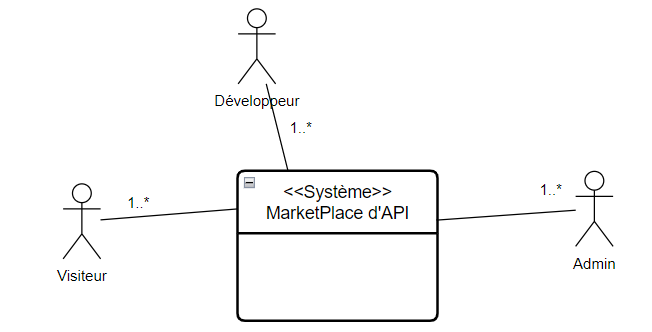
\includegraphics[width=1\columnwidth]{img/Diagramme_de_contexte_statique.png}}
        \caption{Diagramme de contexte statique }
        \label{fig:logo_tt}
    \end{figure}

\pagebreak

    \subsection{Diagramme de cas d’utilisation}
    La figure, ci-dessous, illustre le diagramme de cas d’utilisation du premier sprint sachant qu’un  utilisateur est un acteur fictif pouvant être soit un développeur, soit un administrateur. Il peut consulter les APIs et gérer son profil.
    
    \begin{figure}[H]
        \centering
        \frame{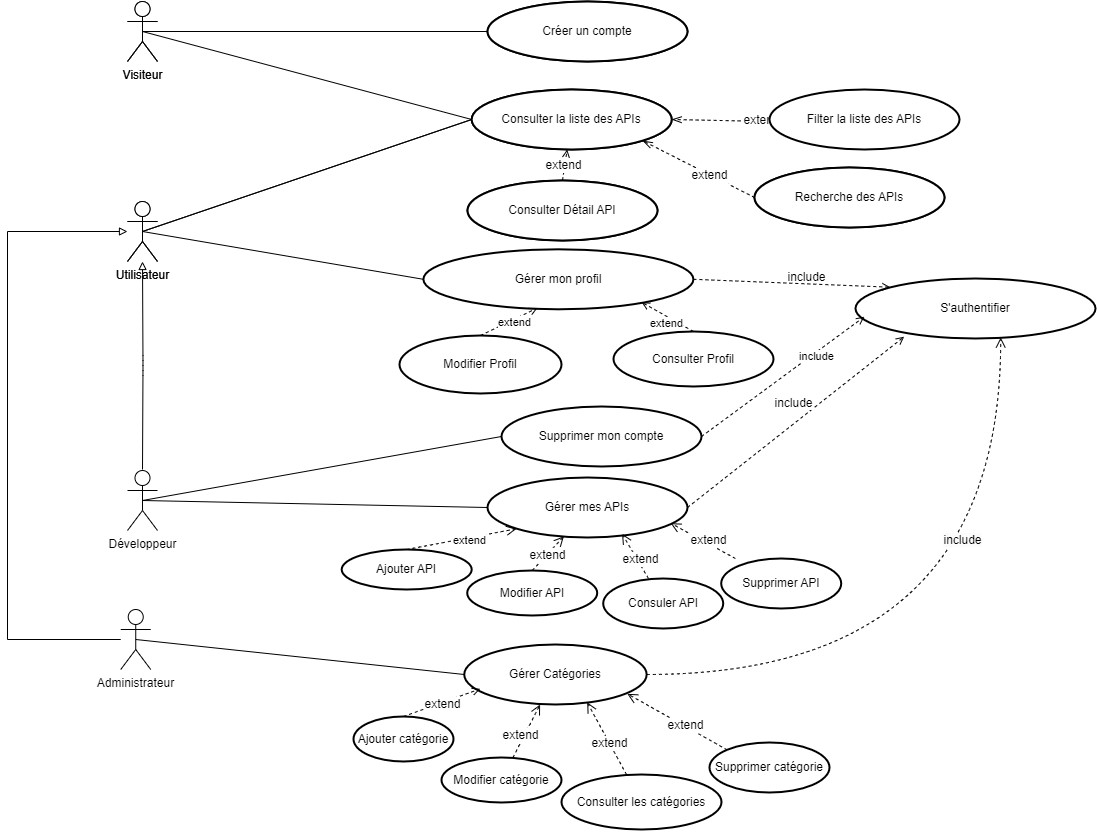
\includegraphics[width=1.1\columnwidth]{Diagramme_de_cas_d'utilisation_du_sprint_1.jpg}}
        \caption{Diagramme de cas d'utilisation du sprint 1 }
        \label{fig:logo_tt}
    \end{figure}
\pagebreak
    \subsection{Exemple d’une maquette d’interface}
    La figure suivante représente la maquette de l’interface de consultation de la liste des APIs de la marketplace  
    \begin{figure}[H]
        \centering
        \frame{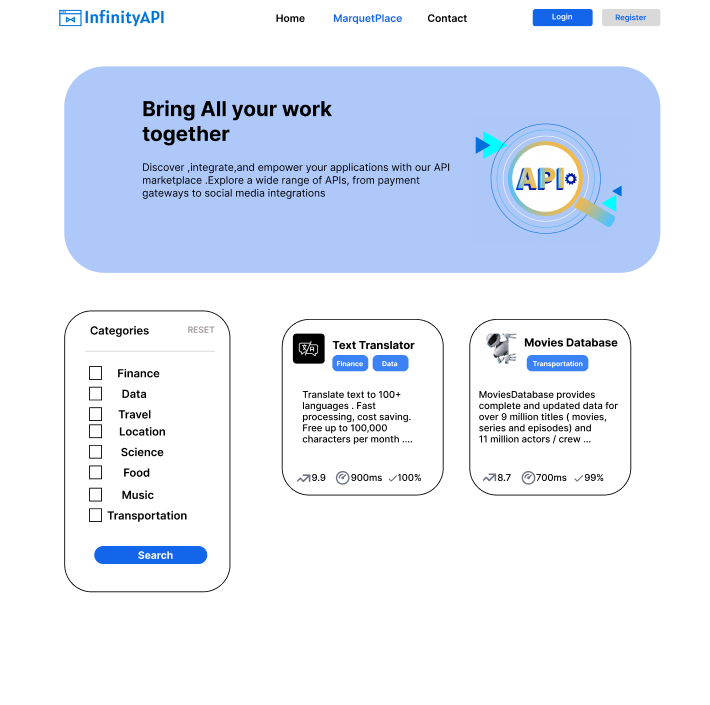
\includegraphics[width=1\columnwidth]{Maquette_de_l'interface_liste_des_APIs.png}}
        \caption{Maquette de l'interface liste des APIs }
        \label{fig:logo_tt}
    \end{figure}
\pagebreak

\section{Conception}
Dans cette partie, nous présentons le diagramme de classes, le diagramme d'activités, et enfin, les diagrammes de séquence.

    \subsection{Modélisation structurelle}

        \subsubsection{Règles de gestion}
        Voici les principales règles de gestion avant de présenter le diagramme de classes :
        \begin{itemize}
            \item  Un administrateur et un développeur sont des utilisateurs.
            \item Un développeur peut fournir zéro ou plusieurs APIs.
            \item Une API peut être fournie par un seul développeur.
            \item Une API peut appartenir à une ou plusieurs catégories.
            \item Une catégorie concerne zéro ou plusieurs APIs
        \end{itemize}

        \subsubsection{Description des principales classes}
        Notre diagramme est composé de plusieurs classes qui interagissent entre elles. Il est possible de distinguer :

        \begin{itemize}
            \item La classe “Developper” stocke les informations de base sur le développeur inscrit dans notre Marketplace telles que son nom, son prénom, le mot de passe et l'e-mail.
            \item La classe “API” stocke les informations de base sur les APIs disponibles dans le système, telles que le nom, la description et l'URL. Elle facilite la gestion et l'accès aux APIs pour les développeurs.
            \item La classe "Category" stocke les informations sur les catégories auxquelles les APIs appartiennent telles que le nom de la catégorie et une description pour aider à organiser les APIs et à faciliter la recherche et la navigation pour les utilisateurs.
        \end{itemize}
    \pagebreak

        \subsubsection{Diagramme de classes}
        Le diagramme de classes se présente comme suit :
        \begin{figure}[H]
            \centering
            \frame{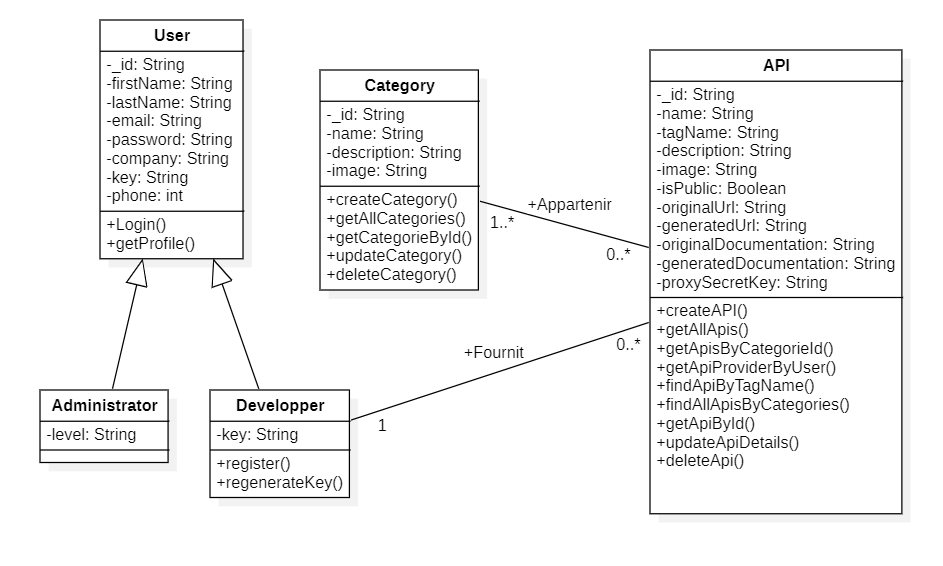
\includegraphics[width=1\columnwidth]{Diagramme_de_classe_du_sprint1.png}}
            \caption{ Diagramme de classes du sprint 1 }
            \label{fig:logo_tt}
        \end{figure}

        \subsubsection{La représentation NoSQL associée à la base de données de la MarketPlace d’API}
        Nous avons opté pour une base de données NoSQL pour notre marketplace d’API car elle s’adapte facilement aux changements, contrairement aux bases de données SQL qui sont moins flexibles. \\
        De plus, NoSQL gère mieux les grandes quantités de données complexes et assure que notre service reste disponible sans interruption, ce qui est essentiel pour répondre efficacement à la forte demande de notre plateforme dynamique.\\
        Par rapport au coût, NoSQL offre des solutions open-source disponibles sur le marché permettant de réduire considérablement les coûts de stockage et de maintenance par rapport aux bases de données SQL.\\
        Ainsi, notre base de données comporte 3 collections pour notre premier sprint. \\
    \pagebreak

        Elle se présente comme suit :
        
        \begin{figure}[H]
            \centering
            \frame{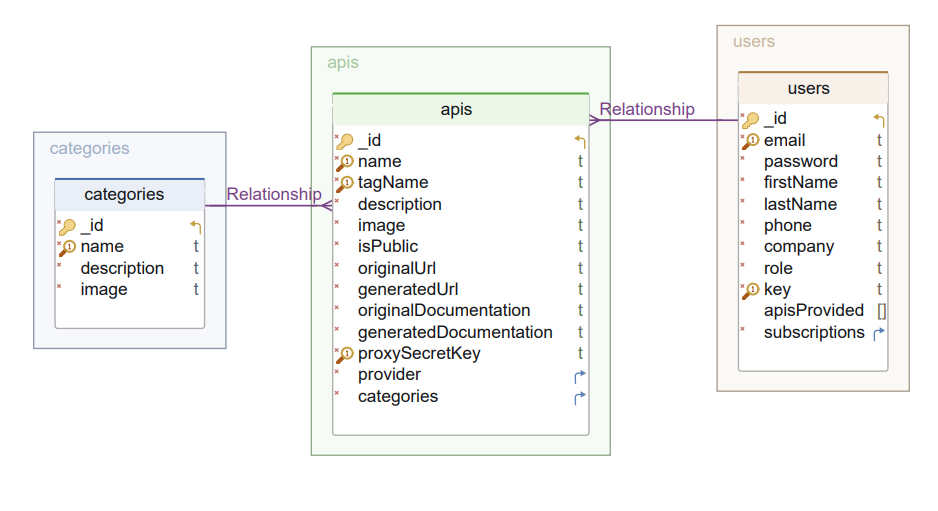
\includegraphics[width=0.8\columnwidth]{Représentation_de_la_base_de_données_du_sprint1.png}}
            \caption{ Représentation de la base de données du sprint 1 }
            \label{fig:logo_tt}
        \end{figure}

    \subsection{Diagramme d’activités "Ajouter API"}

 
    Le diagramme d’activités suivant représente le processus de création d'une API. Un développeur soumet les détails de l'API via un formulaire. Le système vérifie ensuite la validité du jeton JWT pour authentifier l'accès à la fonctionnalité de création d'API. Si le jeton est valide, le système récupère les détails de l'utilisateur et vérifie son existence. \\
    Si l'utilisateur n'existe pas, il est redirigé vers la page d'authentification. Sinon, le système vérifie la validité des détails de l'API. Il s'assure également que le nom et le tag de l'API ne sont pas déjà utilisés. Si les détails sont valides et uniques, une nouvelle URL de consommation unique est générée. Cette URL est utilisée par les consommateurs pour accéder à l'API et à ses fonctionnalités. L'URL est générée à l'aide d'un algorithme qui garantit qu'elle est unique et sécurisée. \\
    Le système vérifie ensuite le chargement correct du fichier Swagger/OpenAPI de documentation. Si le fichier n'est pas correctement chargé, un message d'erreur est affiché. Sinon, la documentation est sauvegardée et validée. La documentation Swagger/OpenAPI est ensuite analysée et mise à jour en fonction de la version du fichier. La nouvelle documentation est ensuite sauvegardée. \\
    Après la génération de la clé secrète unique pour l'API, celle-ci est associée de manière sécurisée à l'API dans la base de données, ce qui constitue une couche supplémentaire de sécurité, assurant que seules les requêtes munies de cette clé secrète peuvent interagir avec l'API. \\
    Enfin, tous les détails de l'API sont enregistrés dans la base de données et un message de succès est affiché. \\

    \begin{figure}[H]
        \centering
        \frame{\includegraphics[width=0.95\columnwidth]{Diagramme_d'activités_Ajouter_API.jpg}}
        \caption{ Diagramme d'activités "Ajouter API"}
        \label{fig:logo_tt}
    \end{figure}

    \subsection{Diagrammes de séquence}

    \subsubsection{Diagramme de séquence "Ajouter API"}

    Le diagramme de séquence décrit le processus de création d'une API. 
    Le développeur soumet une demande via l'interface "API\_Create". Le contrôleur "APIcreate" valide les champs soumis et utilise le service Angular "API" pour envoyer les requêtes au backend. Le middleware "middlewareAuth" vérifie les jetons d'authentification. Le contrôleur du backend "API" orchestre la création de l'API en utilisant les modèles "API" et "User". Une fois l'API est créée, une réponse est renvoyée au service du front pour affichage.
    
    \begin{figure}[H]
        \centering
        \frame{\includegraphics[width=1.1\columnwidth]{  Diagramme_de_séquence_de_conception_AjouterAPI.jpg }}
        \caption{   Diagramme de séquence de conception "Ajouter une API"
        }
        \label{fig:logo_tt}
    \end{figure}
    \pagebreak

\subsection{Diagramme de séquence "Ajouter une catégorie"}
Ce diagramme de séquence illustre la séquence d'interactions entre les différents composants de la marketplace pour ajouter une catégorie. L'administrateur remplit le formulaire d'ajout d'une catégorie. Si les champs sont invalides, un message d'erreur est affiché. Sinon, une requête HTTP est envoyée au backend. Le backend vérifie alors la validité du jeton. Si le jeton est invalide, un message d'erreur "invalid token" est renvoyé. Sinon, le backend vérifie si la catégorie existe déjà. Si tel est le cas, une interface affiche un message d'erreur "category already exists". Sinon, un message de succès est affiché pour indiquer que la catégorie a été ajoutée avec succès.
\begin{figure}[H]
    \centering
    \frame{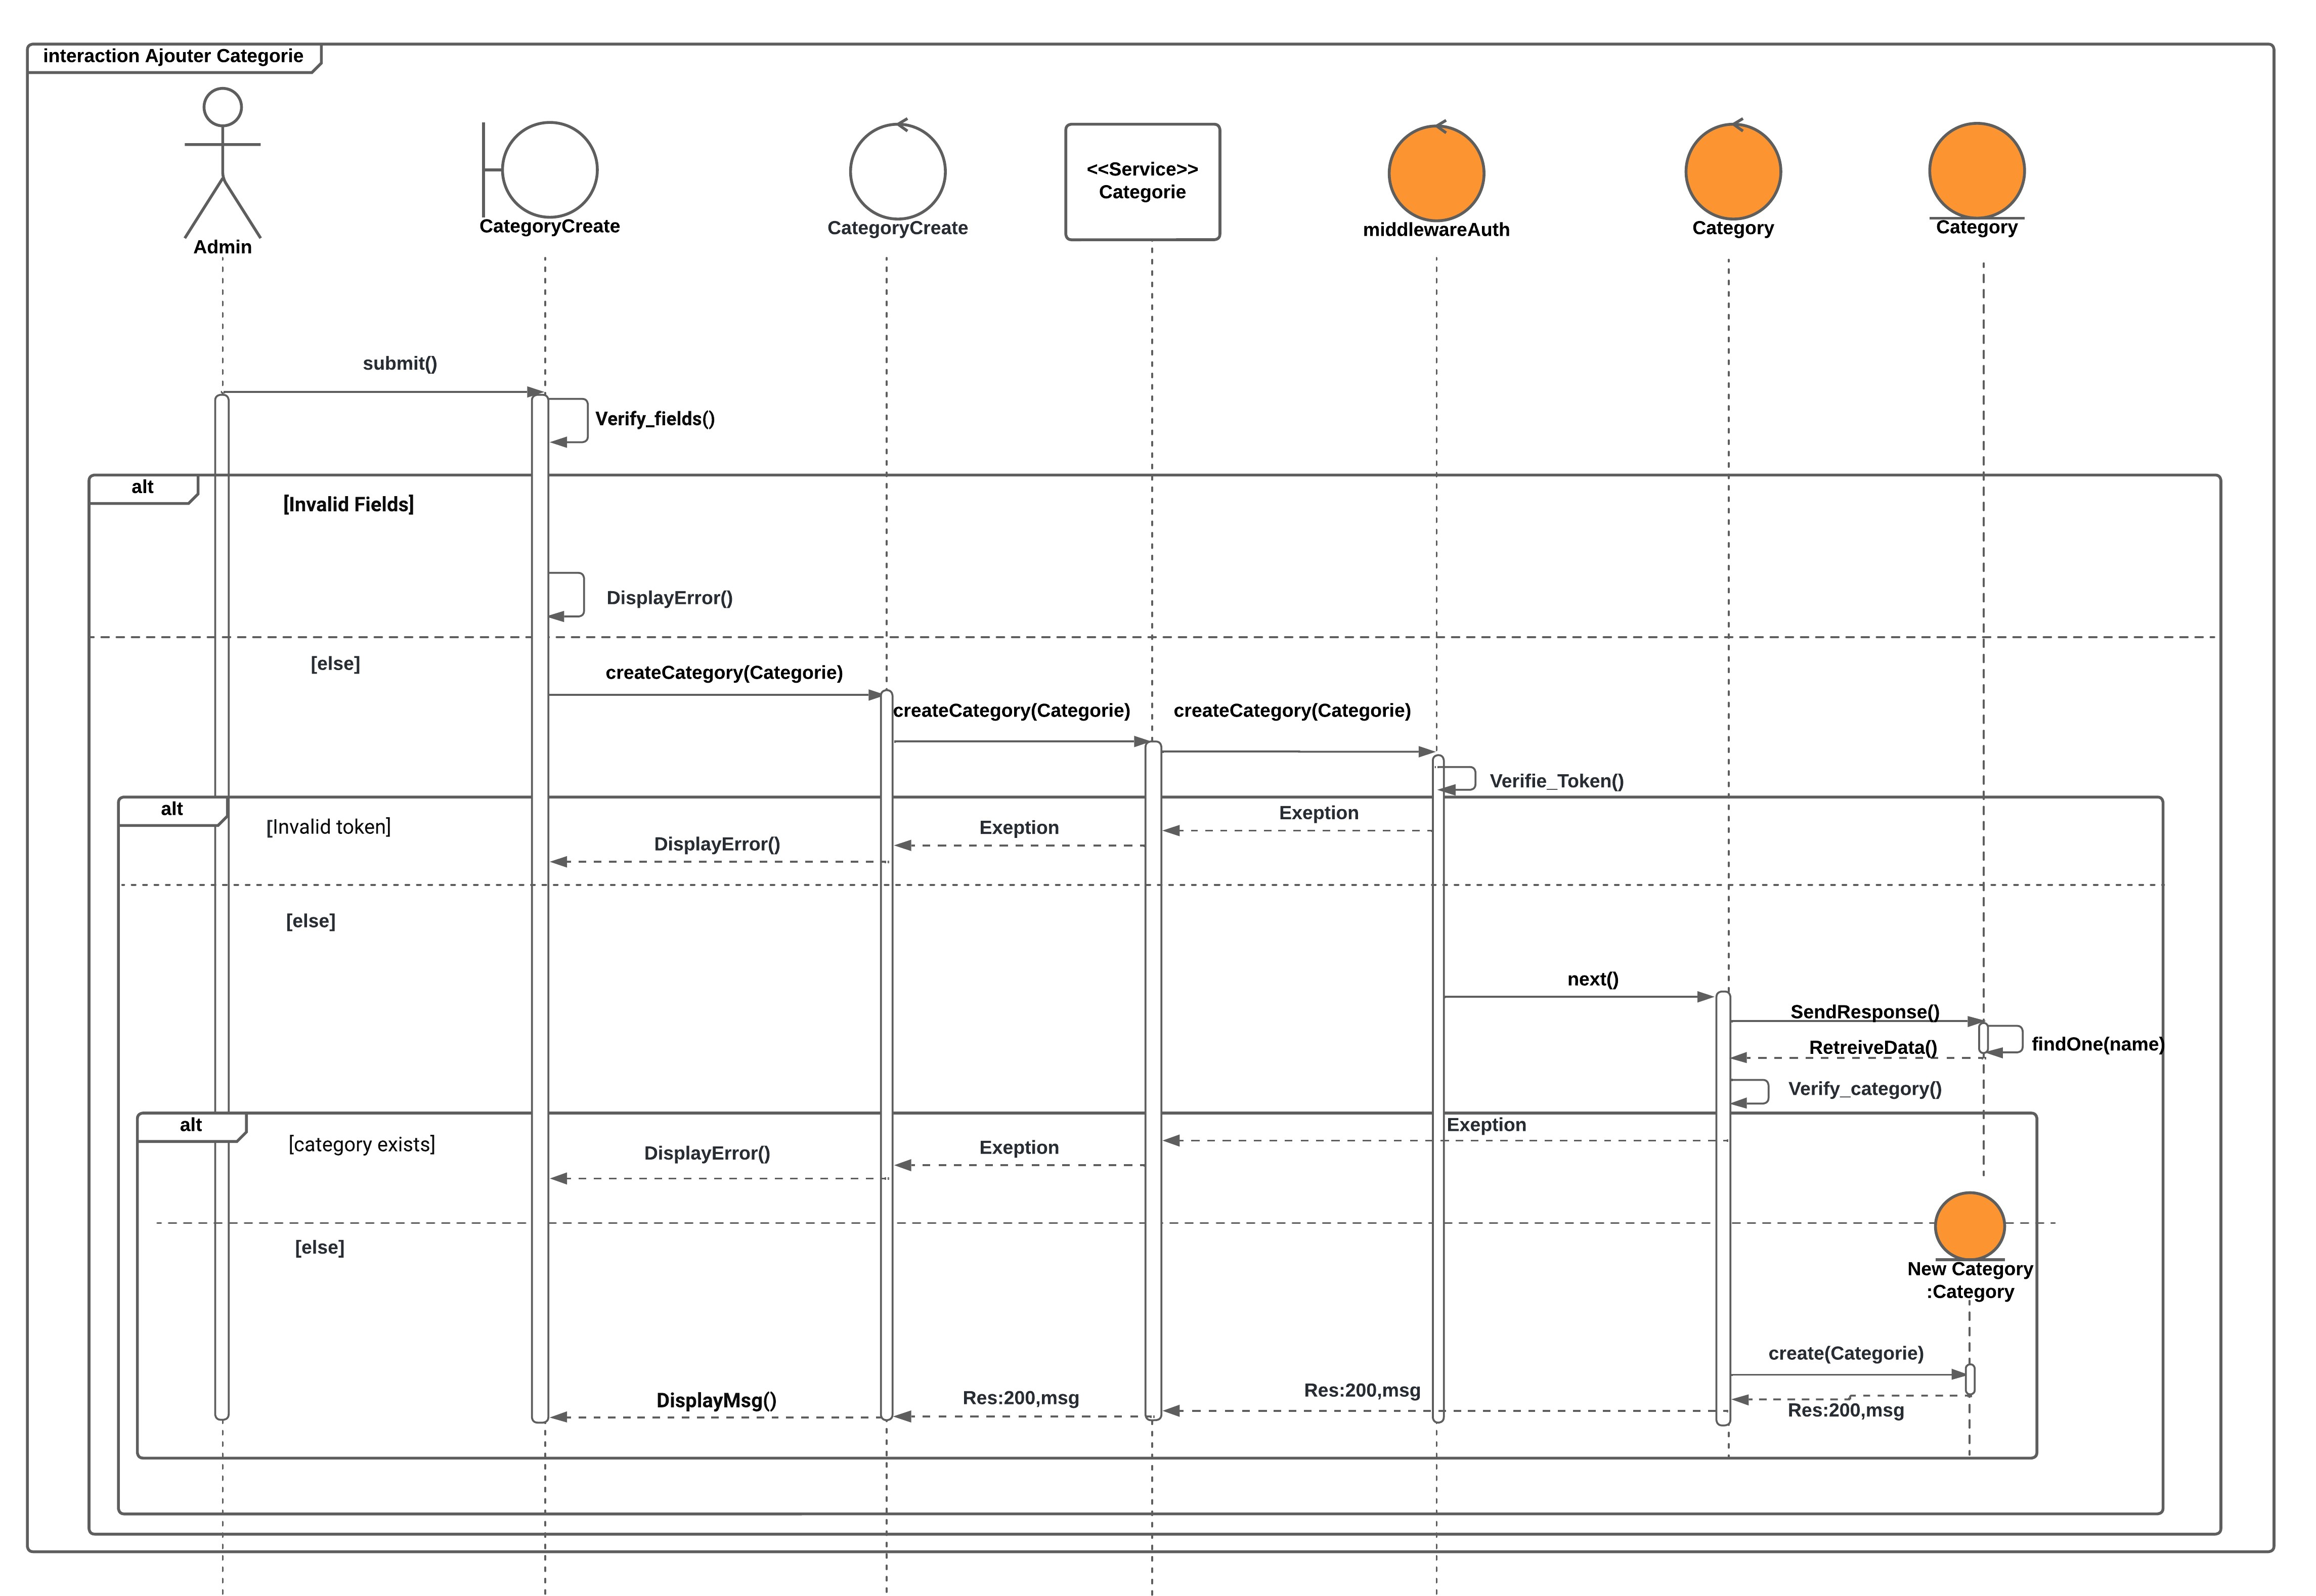
\includegraphics[width=1.1\columnwidth]{  Diagramme_de_séquence_Ajoutercatégorie.jpg}}
    \caption{ Diagramme de séquence "Ajouter une catégorie" }
    \label{fig:logo_tt}
\end{figure}
 \pagebreak



  
    \section{Revue de sprint}
    La revue du premier sprint expose le travail réalisé au niveau du sprint 1. Elle est divisée en deux parties : la réalisation et le burndown chart du projet.
    \subsection{Réalisation }
    Dans cette partie, nous allons présenter les interfaces réalisées au niveau du sprint 1.
    \subsubsection{Création du compte développeur et l'authentification}
        Cette interface présente la page de création d'un compte développeur 
        \begin{figure}[H]
            \centering
            \frame{\includegraphics[width=1\columnwidth]{Interfacedecréationdecompte.png}}
            \caption{Interface de création de compte}
            \label{fig:logo_tt}
        \end{figure}
    \pagebreak

        Cette interface présente la page d’authentification
        \begin{figure}[H]
            \centering
            \frame{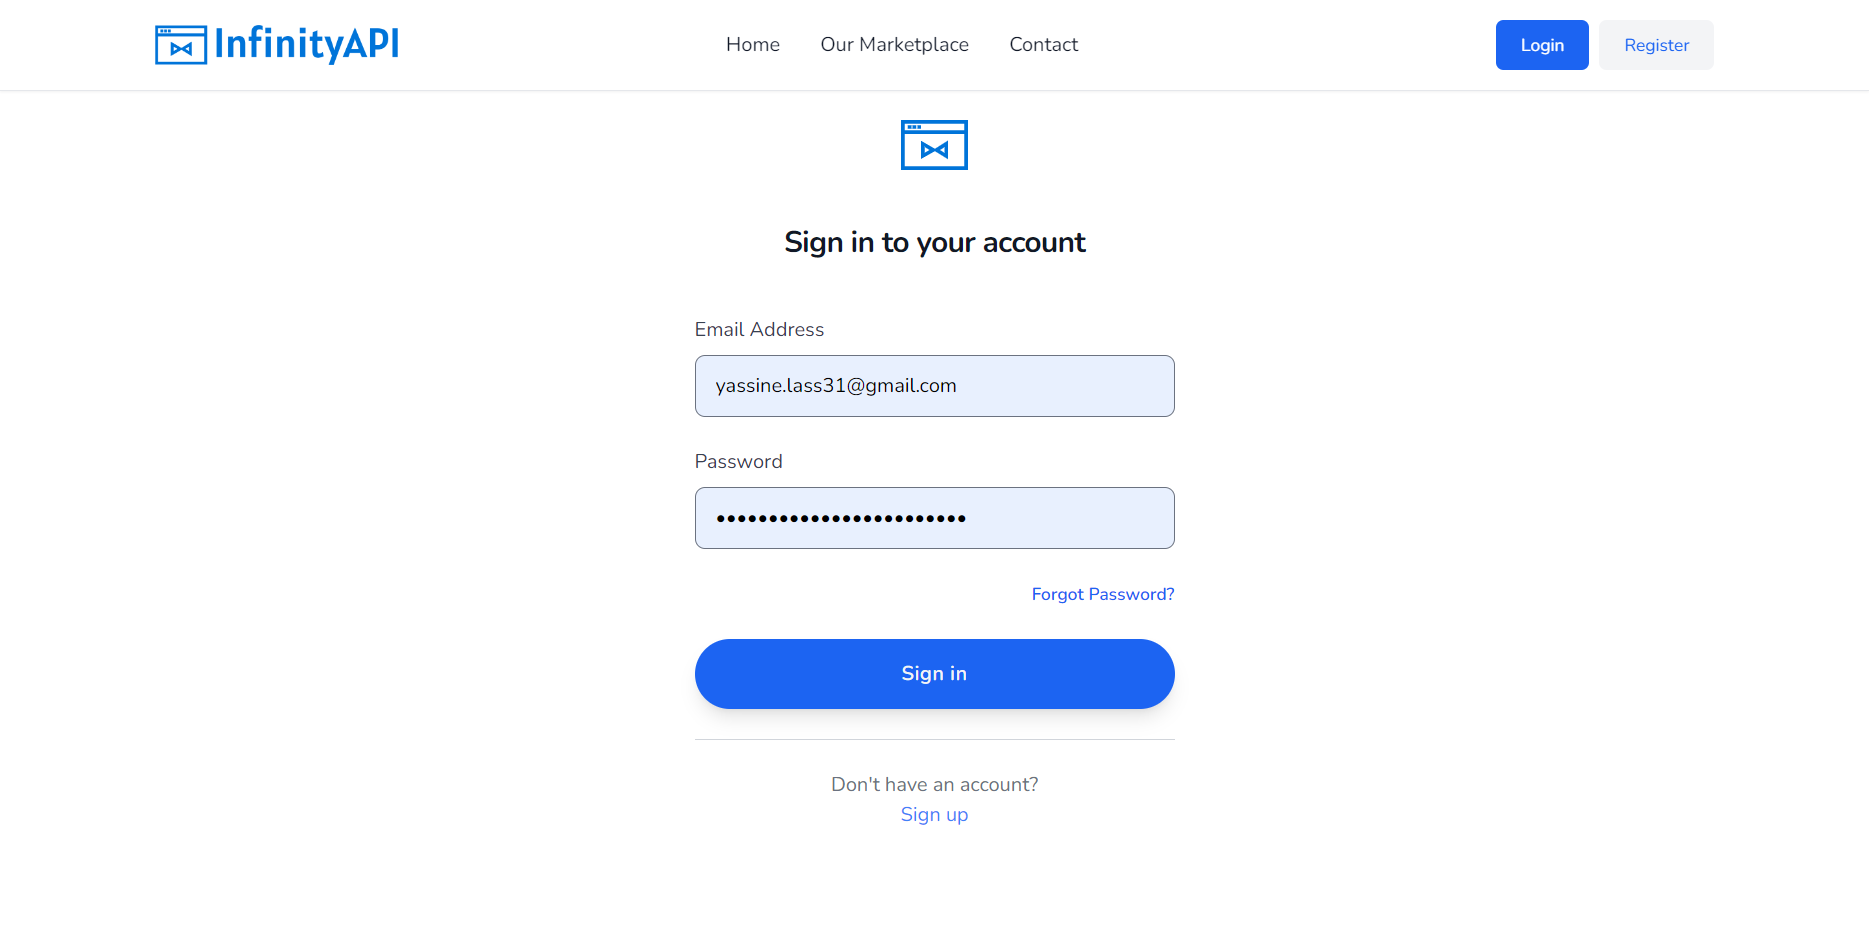
\includegraphics[width=0.8\columnwidth]{Interface_dauthentification.png}}
            \caption{Interface d'authentification}
            \label{fig:logo_tt}
        \end{figure}

    \subsubsection{Gestion des APIs  }
    Cette interface présente la page d'ajout d'une API
    \begin{figure}[H]
        \centering
        \frame{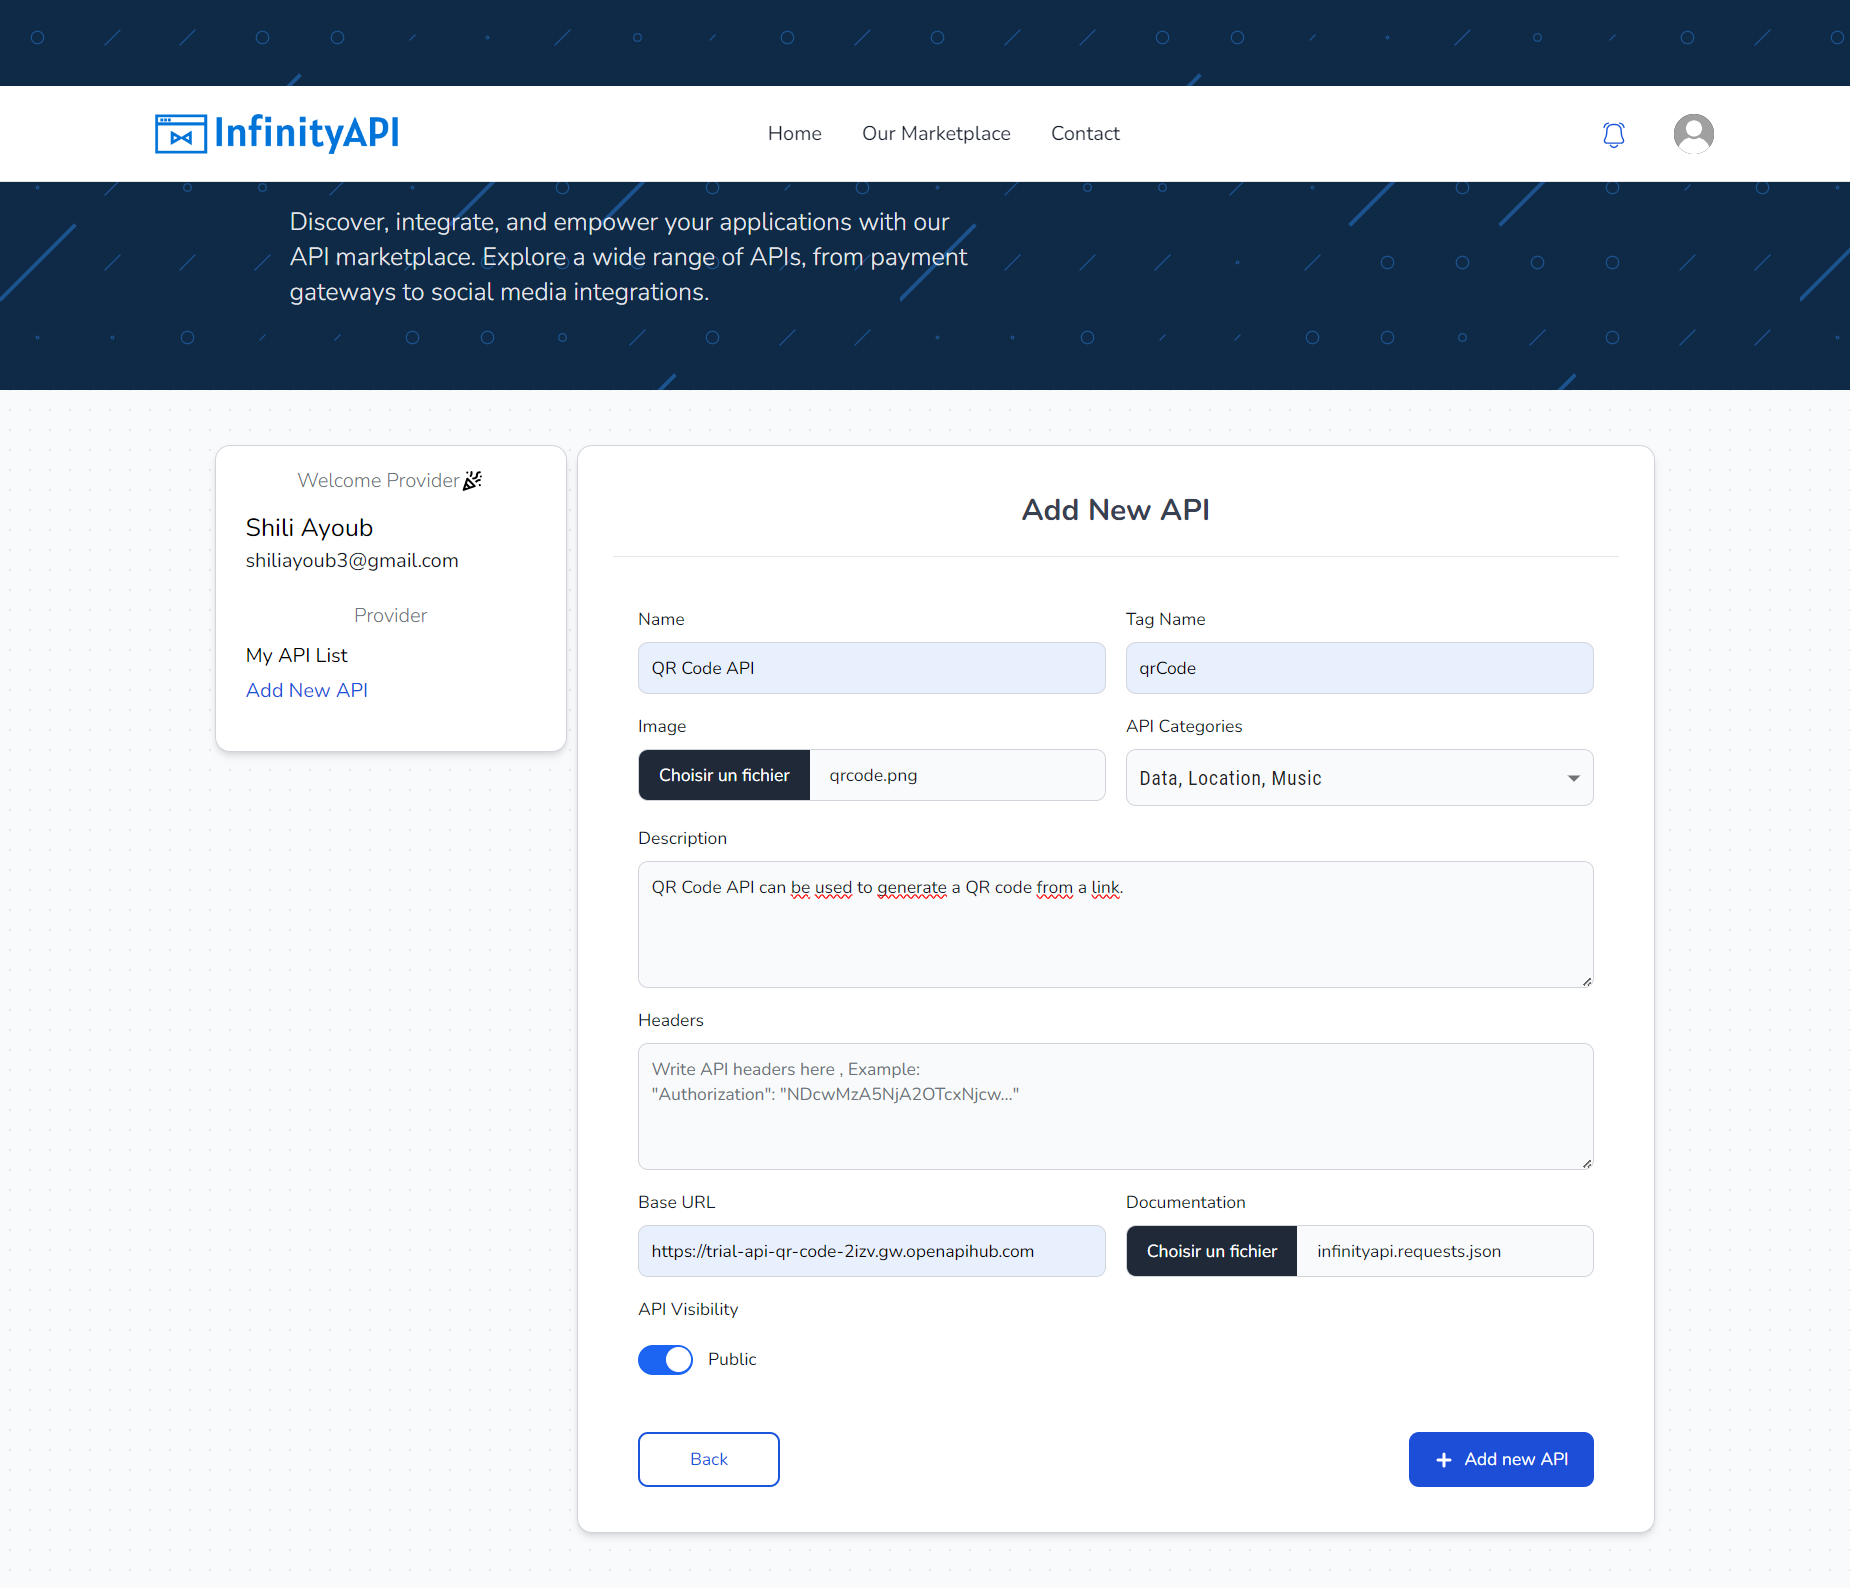
\includegraphics[width=0.85\columnwidth]{    Interface_dajout_dune_API.png        }}
        \caption{Interface d'ajout d'une API }
        \label{fig:logo_tt}
    \end{figure}
    \pagebreak


    \subsubsection{Affichage de la liste des APIs de la marketplace }	
    Cette interface présente la page de la liste des APIs consultable par le public.
    \begin{figure}[H]
        \centering
        \frame{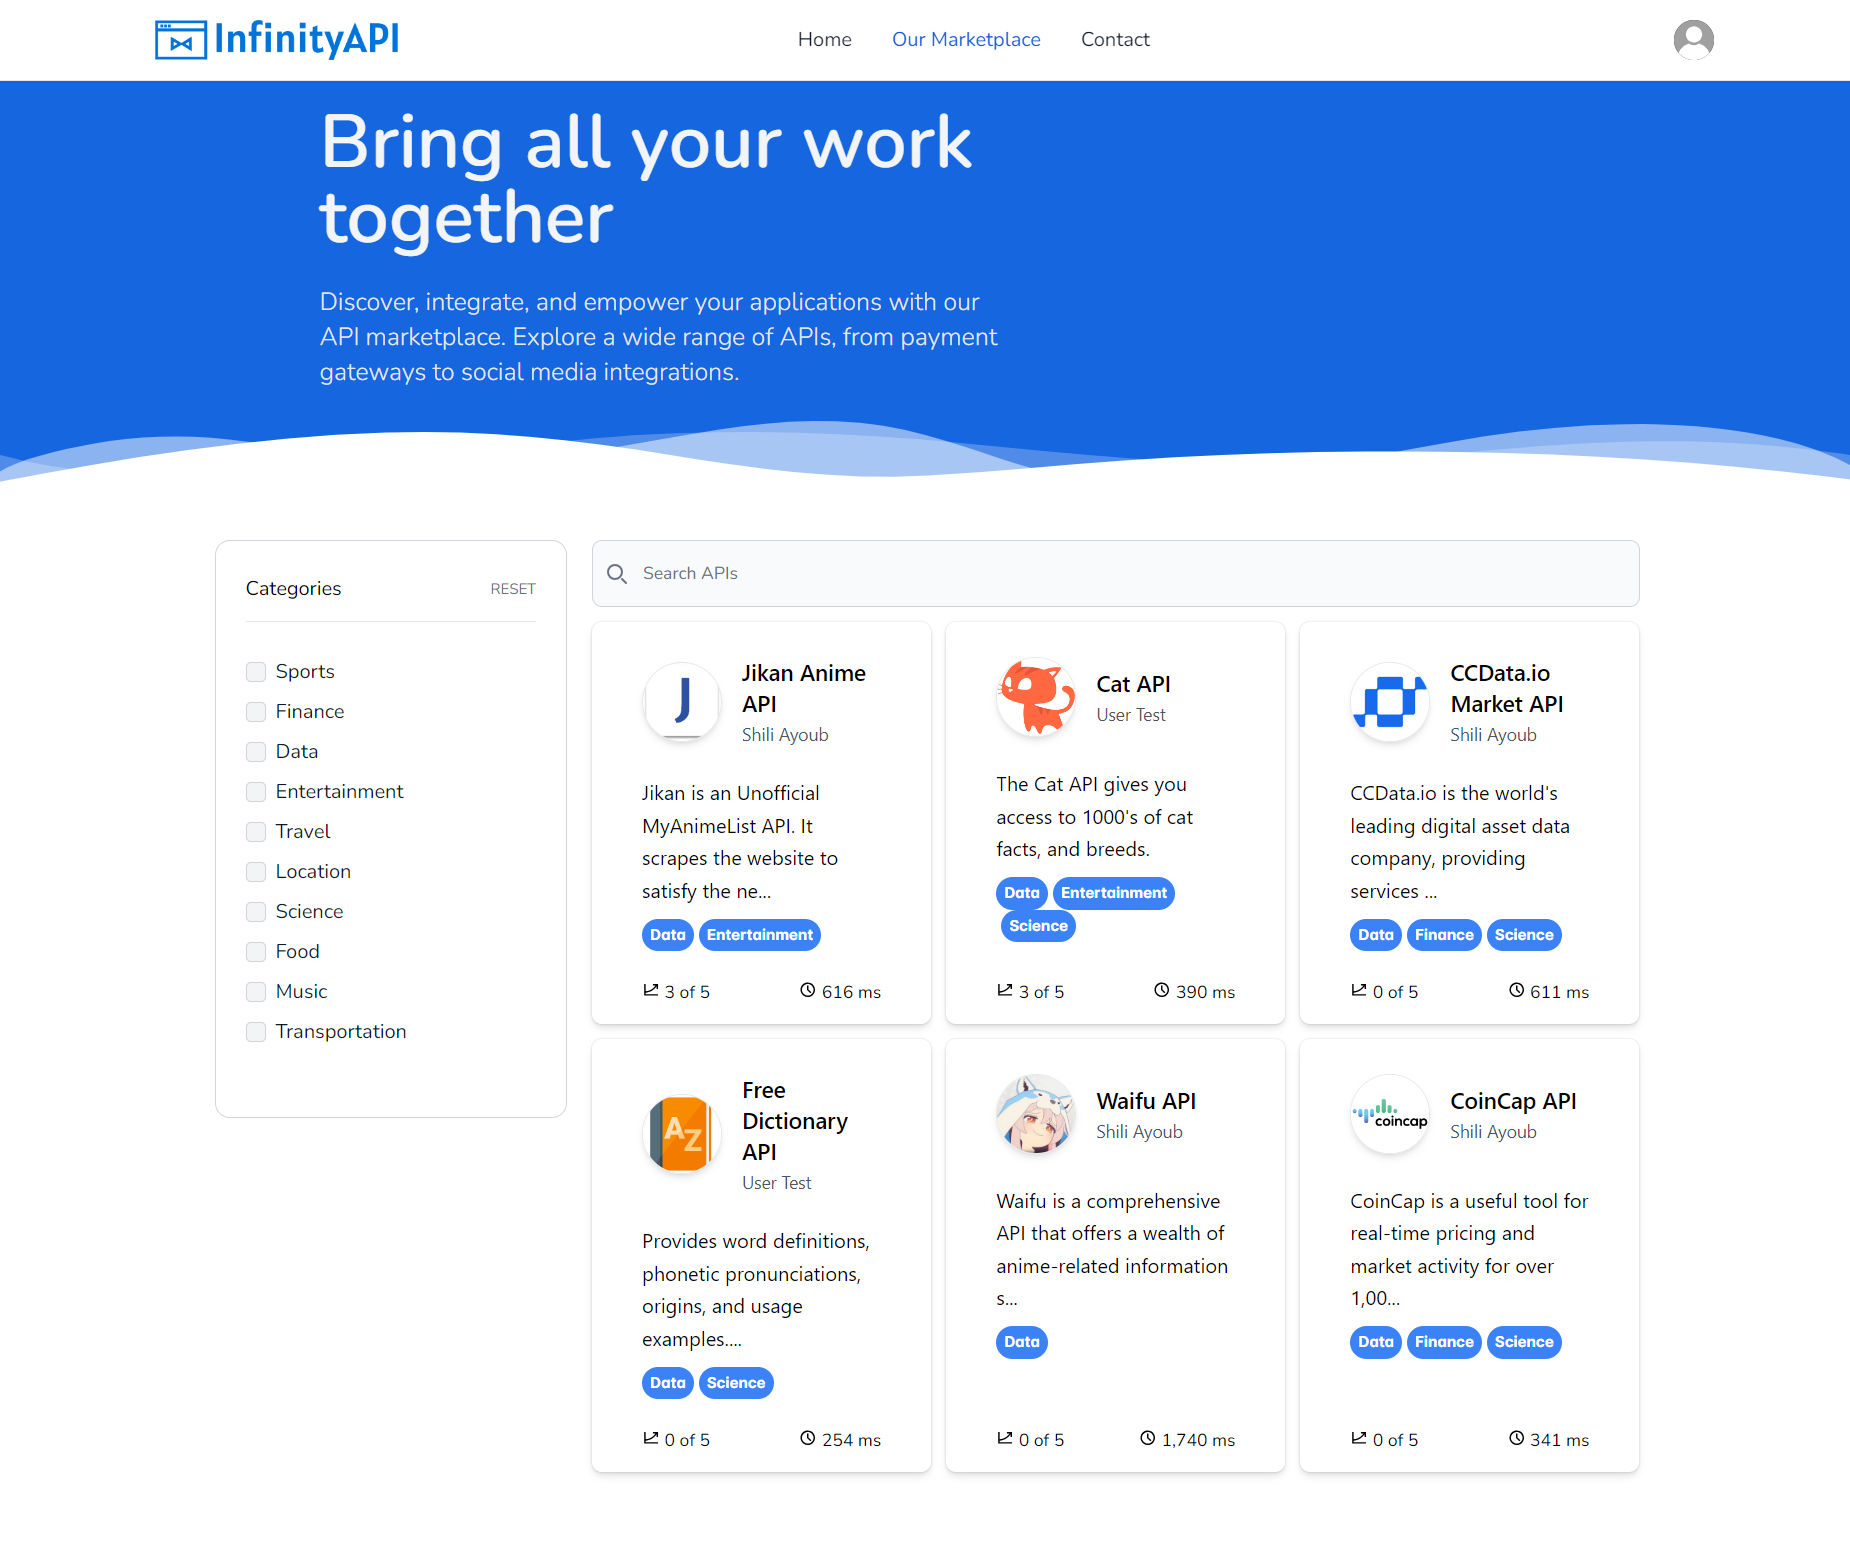
\includegraphics[width=0.7\columnwidth]{ Interface_de_liste_des_APIs.png}}
        \caption{ Interface de liste des APIs }
        \label{fig:logo_tt}
    \end{figure}
    \subsubsection{Affichage de la Documentation d'une API dans notre marketplace }	
    
    Cette interface présente la page de la documentation d'une API sélectionnée.
    \begin{figure}[H]
        \centering
        \frame{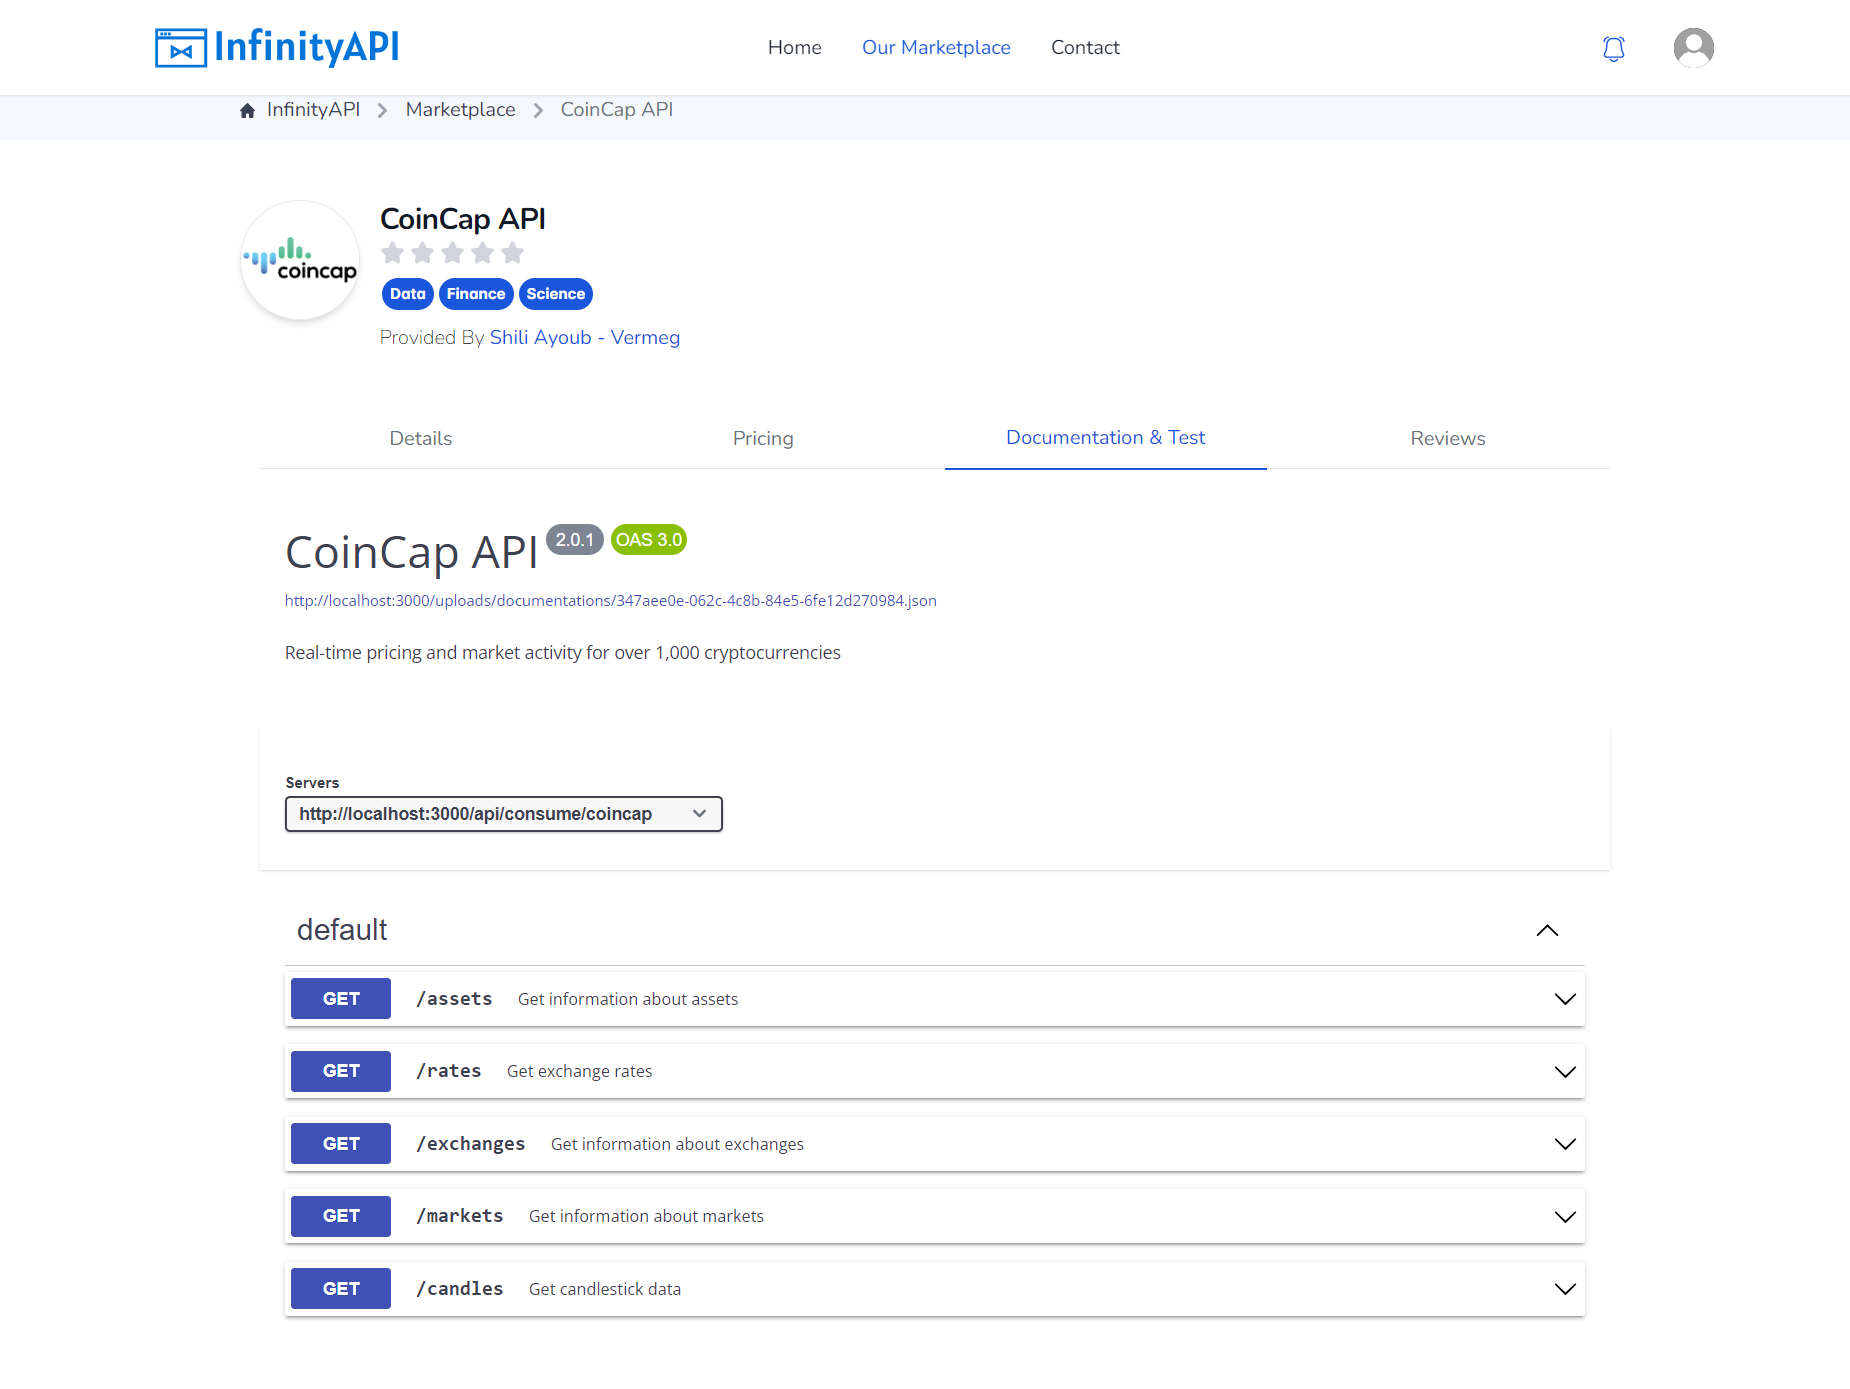
\includegraphics[width=0.7\columnwidth]{ Interface_de_test_de_lAPI.png}}
        \caption{Interface de documentation des endpoints}
        \label{fig:logo_tt}
    \end{figure}
    \pagebreak

    \subsubsection{Gestion du profil utilisateur}	
	Cette interface représente l'interface de gestion du profil développeur.
    \begin{figure}[H]
        \centering
        \frame{\includegraphics[width=0.8\columnwidth]{Interface_de_gestion_du_profil_développeur.png}}
        \caption{Interface de gestion du profil développeur}
        \label{fig:logo_tt}
    \end{figure}  
        Cette interface représente l'interface de gestion du profil administrateur.
        \begin{figure}[H]
            \centering
            \frame{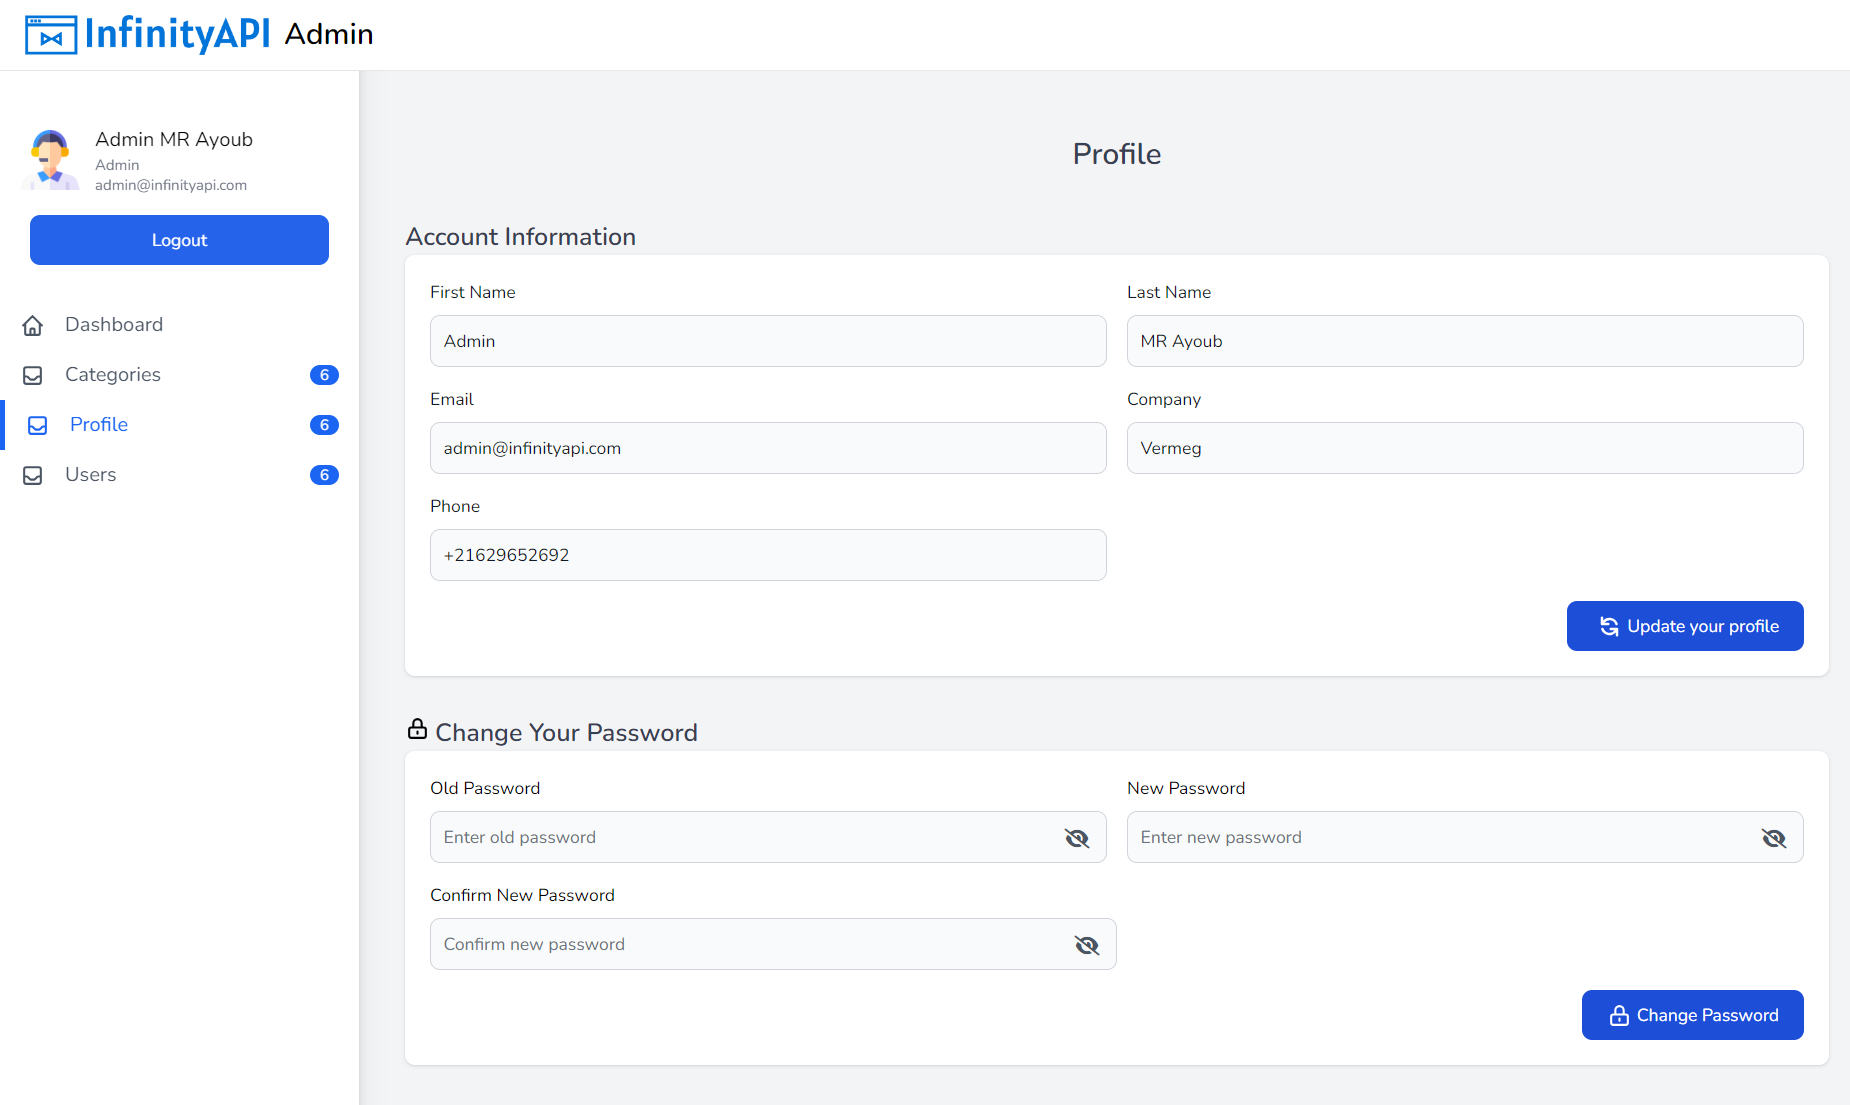
\includegraphics[width=0.8\columnwidth]{Interface_de_gestion_du_profil_administrateur.png}}
            \caption{Interface de gestion du profil d'un administrateur}
            \label{fig:logo_tt}
        \end{figure}

        \subsection{Burndown Chart}	               
        Le burndown chart va nous permettre de suivre la progression d'un projet. Il montre la quantité de travail restant (en terme d'effort estimé) par rapport au temps écoulé comme la montre la figure ci-dessous :
        \begin{figure}[H]
            \centering
            \frame{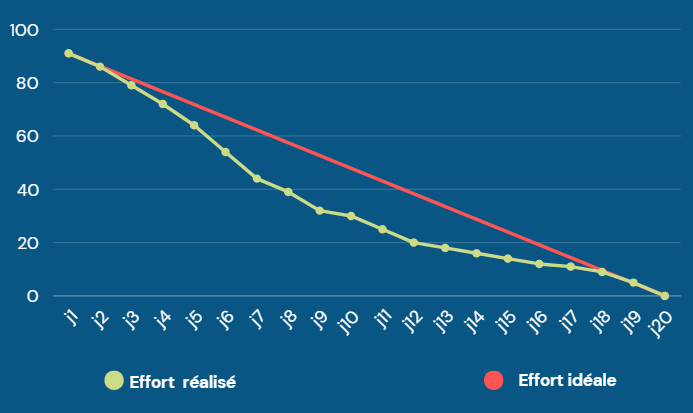
\includegraphics[width=0.9\columnwidth]{Burndown_Chart_du_sprint1.png}}
            \caption{Burndown Chart du sprint 1}
            \label{fig:logo_tt}
        \end{figure}
        
        La courbe présentée indique que nous n'avons pas correctement estimé les efforts des user stories. \\
        La vélocité de notre équipe est évaluée à 91.

        \subsection{     Rétrospective du sprint 1        }	               
        Le tableau, ci-dessous, résume la rétrospective du premier sprint

        
        \begin{longtable}[c]{|p{0.25\linewidth}|p{0.6\linewidth}|}
            \hline
            \textbf{Les questions} & \textbf{Les réponses} \\
            \hline
            \endfirsthead
            \multicolumn{2}{c}%
            {{\bfseries \tablename\ \thetable{} -- suite de la page précédente}} \\
            \hline
            \textbf{Les questions} & \textbf{Les réponses} \\
            \hline
            \endhead
            \hline \multicolumn{2}{|r|}{{\bfseries Suite à la page suivante}} \\
            \hline
            \endfoot
            \hline
            \endlastfoot
        
            \multirow{2}{=}{Ce qui s'est bien passé} & Maîtrise des langages et des logiciels utilisés. \\
            & Achèvement des thèmes \\
            \hline
            Les problèmes rencontrés & Manque d'informations et difficulté concernant l'intégration des APIs dans notre projet. \\
            \hline
            Les choses à améliorer & Mieux organiser les tâches à faire entre nous. \\
            \hline
        \end{longtable}
 
\section*{Conclusion}
Dans ce chapitre, nous avons présenté la partie spécification fonctionnelle, conception, ainsi que la revue et la rétrospective du premier sprint. Le deuxième sprint est abordé dans le chapitre suivant.


        \clearpage
        
        \chapter{Sprint 2 "Gestion de la tarification, souscription et consommation d'une API"}
	
\section*{Introduction}
Après avoir présenté dans le chapitre précédent le premier sprint, nous abordons, maintenant, le deuxième sprint. Celui-ci suit les mêmes étapes que le chapitre précédent, de la planification à la mise en œuvre, en mettant en exergue le backlog du sprint 2, ainsi que la spécification fonctionnelle, la conception, la revue du sprint et  pour conclure la rétrospective.


\section{ Extrait du backlog du sprint 2}
    Les thèmes du deuxième sprint sont : Gestion de la  tarification, souscription, test et consommation d'une API ainsi  que la gestion des comptes utilisateurs. \\
    Nous allons maintenant présenter un extrait du backlog du sprint à travers les users stories qui traitent la : Consommation d’une API et la souscription à une API  
    \begin{table}[H]
        \centering
        \caption{Extrait du backlog du sprint 2  "Consommation d'une API"}
        \label{tab:task_estimation_subscription}
    \begin{longtable}[c]{|p{0.25\linewidth}|p{0.25\linewidth}|p{0.25\linewidth}|p{0.15\linewidth}|}
        \hline
        \textbf{User story} & \textbf{Tâches} & \textbf{Sous-tâches} & \textbf{Estimation} \\
        \hline
        \endfirsthead
        \multicolumn{4}{c}%
        {{\bfseries \tablename\ \thetable{} -- suite de la page précédente}} \\
        \hline
        \textbf{User story} & \textbf{Tâches} & \textbf{Sous-tâches} & \textbf{Estimation} \\
        \hline
        \endhead
        \hline \multicolumn{4}{|r|}{{\bfseries Suite à la page suivante}} \\
        \hline
        \endfoot
        \hline
        \endlastfoot

        \multirow{8}{=}{En tant que développeur, je veux pouvoir consommer une API.}
            & Recherche & Documentation & 7\\
        \cline{2-4}
            & \multirow{2}{=}{Modélisation \& conception UML} & Réalisation du diagramme d’activités & 2h \\
        \cline{3-4}
            & & Réalisation du diagramme de séquence & 2h \\
        \cline{2-4}
            & \multirow{2}{=}{Préparation du backend} & Réalisation de la fonction post “consumeAPI” & 10h \\
        \cline{3-4}
            & & Test & 1h \\
        \hline
    \end{longtable}
    \end{table}

    \begin{table}[H]
        \centering
        \caption{Extrait du backlog du sprint 2  "Souscription à une API"}
        \label{tab:task_estimation_subscription}
        \begin{longtable}{|p{0.25\linewidth}|p{0.25\linewidth}|p{0.25\linewidth}|p{0.15\linewidth}|}
            \hline
            \textbf{User story} & \textbf{Tâches} & \textbf{Sous-tâches} & \textbf{Estimation} \\
            \hline
            \endfirsthead
            \multicolumn{4}{c}%
            {{\bfseries \tablename\ \thetable{} -- suite de la page précédente}} \\
            \hline
            \textbf{User story} & \textbf{Tâches} & \textbf{Sous-tâches} & \textbf{Estimation} \\
            \hline
            \endhead
            \hline \multicolumn{4}{|r|}{{\bfseries Suite à la page suivante}} \\
            \hline
            \endfoot
            \hline
            \endlastfoot
    
            \multirow{10}{=}{En tant que développeur, je veux pouvoir souscrire à une API pour accéder aux fonctionnalités qu'elle propose.}
                & Préparation de la Maquette & Réalisation de la maquette & 4h \\
            \cline{2-4}
                & Recherche & Documentation & 6h \\
            \cline{2-4}
                & \multirow{1}{=}{Modélisation \& conception UML} & Réalisation du diagramme d’activités & 2h \\
            \cline{2-4}
                & \multirow{2}{=}{Préparation du backend} & Réalisation de la fonction post "createSubscription” & 8h \\
            \cline{3-4}
                & & Test & 2h \\
            \cline{2-4}
                & \multirow{3}{=}{Préparation du frontend} & Modification de l’interface “API plans” & 4h \\
            \cline{3-4}
                & & Validation du formulaire & 1h \\
            \cline{3-4}
                & & Préparation du service “SubscriptionService” & 2h \\
            \cline{3-4}
                & & Préparation de la fonction “onsubmit” & 2h \\
            \cline{3-4}
                & & Test & 1h \\
            \hline
        \end{longtable}
    \end{table}

\section{Spécification fonctionnelle}
Dans cette partie nous allons présenter le diagramme de cas d'utilisation et un exemple de maquette.
  \subsection{Diagramme de cas d'utilisation}
  Dans notre diagramme de cas d'utilisation, nous incluons les nouveaux cas d'utilisation :
  \begin{itemize}
    \item  \textbf{Développeur}
    \begin{itemize}
        \item  Consulter les plans de tarification d'une API.
        \item Gérer mes souscriptions.
        \item Tester une API.
        \item Consommer une API.
        \item Gérer mon profil.
    \end{itemize} 
    \pagebreak

    \item  \textbf{Administrateur}
    \begin{itemize}
        \item Consulter les plans de tarification d'une API.
        \item Consommer une API.
        \item Gérer les développeurs.
        \item Gérer mon profil .
    \end{itemize}
   
\end{itemize}
Deux acteurs secondaires sont introduits au niveau de ce sprint :
\begin{itemize}
    \item \textbf{Le fournisseur de services API} qui héberge les API .
    \item \textbf{Stripe} qui assure le paiement en ligne des souscriptions .
\end{itemize}


\begin{figure}[H]
    \centering
    \frame{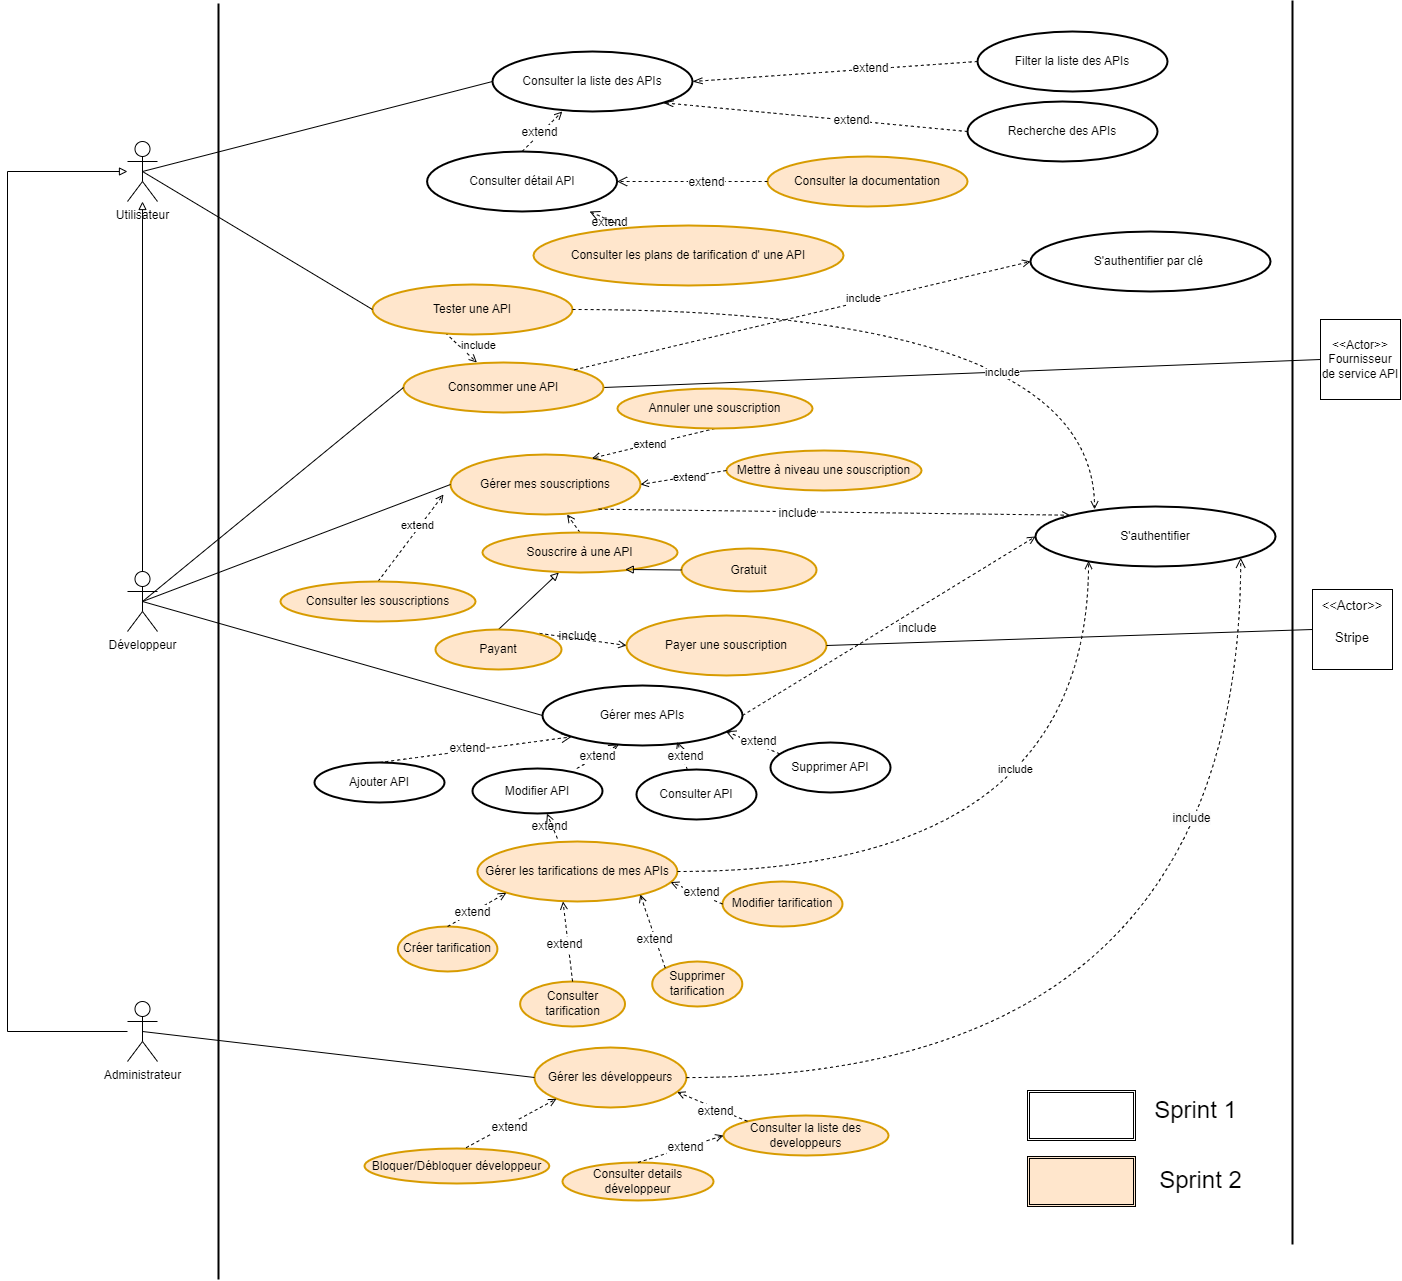
\includegraphics[width=1.1\columnwidth]{diagrammedecasdutilisationsprint2.png}}
    \caption{Diagramme de cas d'utilisation du sprint2}
    \label{fig:logo_tt}
\end{figure} 
\pagebreak

\subsection{Exemple d'une maquette d'interface du sprint 2 }
La figure suivante représente la maquette de l'interface d'ajout d'un plan de tarification dans la marketplace.
\begin{figure}[H]
    \centering
    \frame{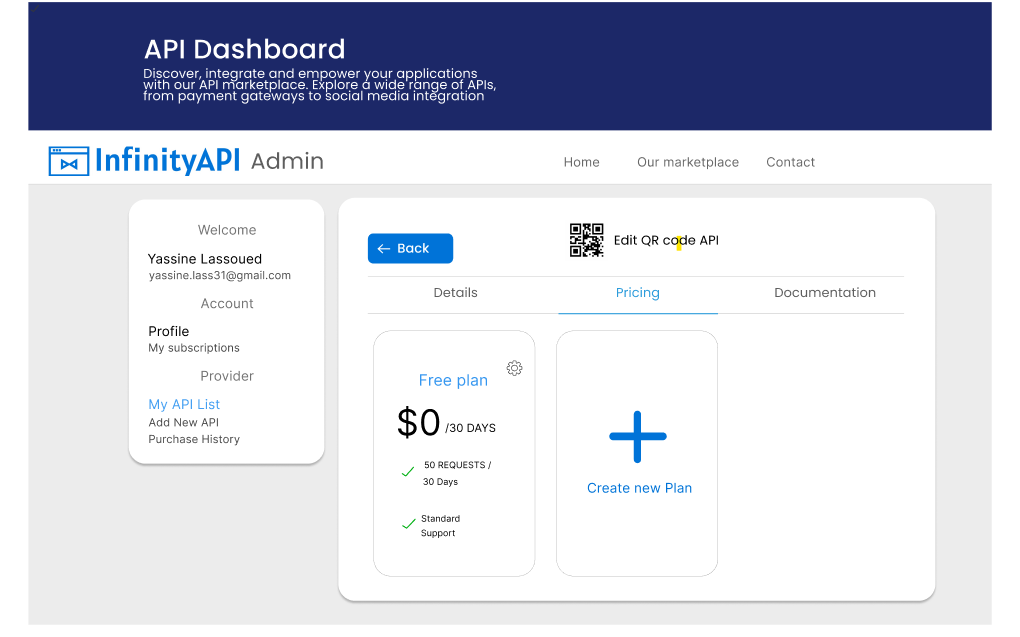
\includegraphics[width=1.1\columnwidth]{maquettetarificationAPI.png}}
    \caption{Maquette d'ajout d'un plan de tarification}
    \label{fig:logo_tt}
\end{figure}
\pagebreak

\section{Conception}
Dans cette partie, nous présentons le diagramme de classes, les diagrammes d'activités ainsi que les diagrammes de séquence afin d'illustrer les traitements des user stories clés de ce sprint, à savoir : l'ajout d'un plan de tarification, la souscription à une API et la consommation d'une API .
\subsection{Modélisation structurelle}

\subsubsection{Règles de gestion et de calcul}
Voici les principales règles de gestion avant de présenter le diagramme de classes :
\begin{itemize}
    \item  Une souscription peut être associée à zéro ou un paiement.
    \item Un paiement appartient à une seule souscription.
    \item Une souscription est effectuée pour un seul plan.
    \item Un plan peut être associé à zéro ou plusieurs souscriptions.
    \item Une requête est faite par un seul utilisateur.
    \item Un utilisateur peut déposer zéro ou plusieurs requêtes.
    \item Le pourcentage de commission de la plateforme est évalué à 15\%.
\end{itemize}

\subsubsection{Diagramme de classes}
\begin{figure}[H]
    \centering
    \frame{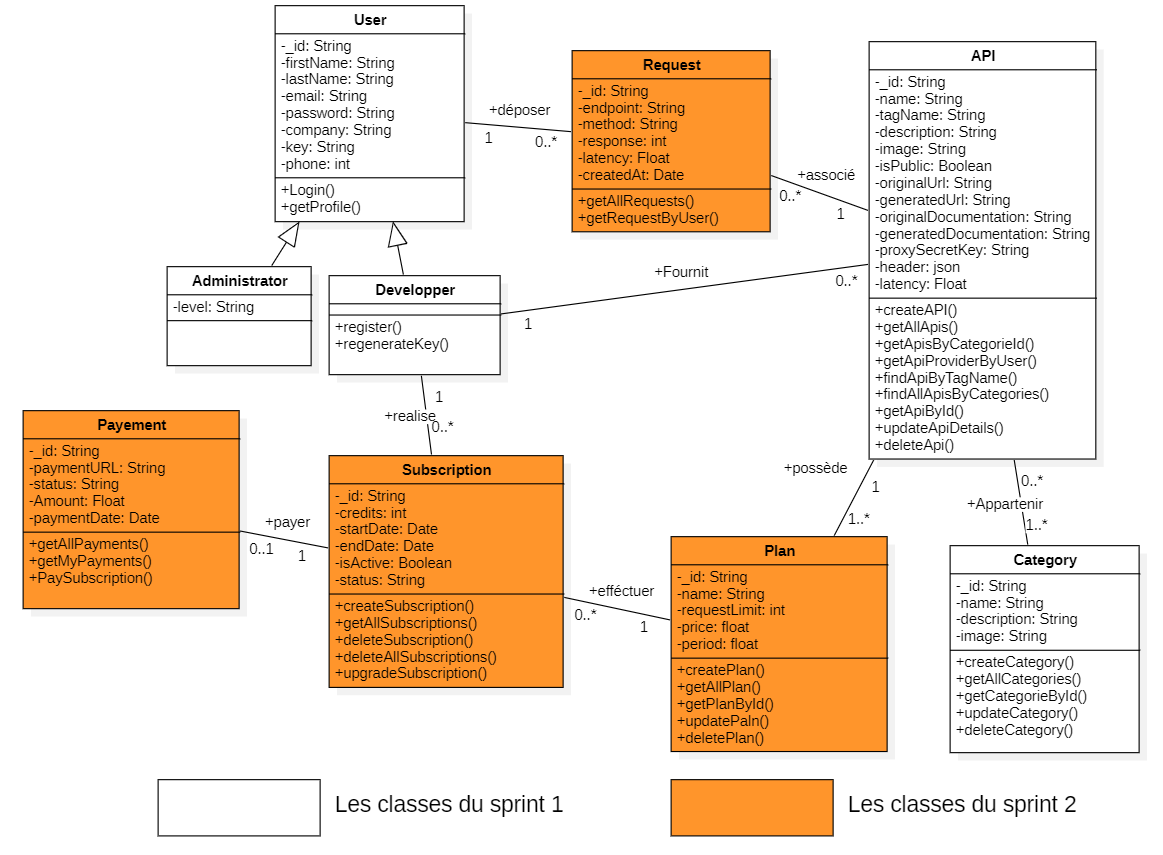
\includegraphics[width=0.8\columnwidth]{DiagrammeDeClasseDeSprint2.png}}
    \caption{Diagramme de classes du sprint 2}
    \label{fig:logo_tt}
\end{figure}
\pagebreak

\subsection{Diagramme d'activités "Ajouter un plan de tarification"}
Ce diagramme d'activités représente le processus de création d'un plan de tarification. Initialement, un développeur soumet les détails du plan via un formulaire. Ensuite, le système vérifie la validité du jeton JWT pour authentifier l'accès à l'API de tarification. \\
 Si le jeton est valide, le système procède à la vérification de l'existence de l'utilisateur. Si l'utilisateur n'existe pas, il est redirigé vers la page d'authentification. Sinon, le système vérifie si l'utilisateur est le fournisseur de l'API. \\
S'il est le fournisseur, le système vérifie l'unicité du nom  du plan ainsi que le prix .Si une quelconque condition n'est pas satisfaite, un message d'erreur est affiché. Sinon, le système vérifie si le nombre maximal de plans de tarification est dépassé. S'il est dépassé, une erreur est affichée. Une erreur sera également signalée si le nombre de requêtes ou la période correspondent déjà à un autre plan. Si aucune erreur n'est détectée, le plan est ajouté avec succès et un message de réussite est affiché.
\begin{figure}[H]
    \centering
    \frame{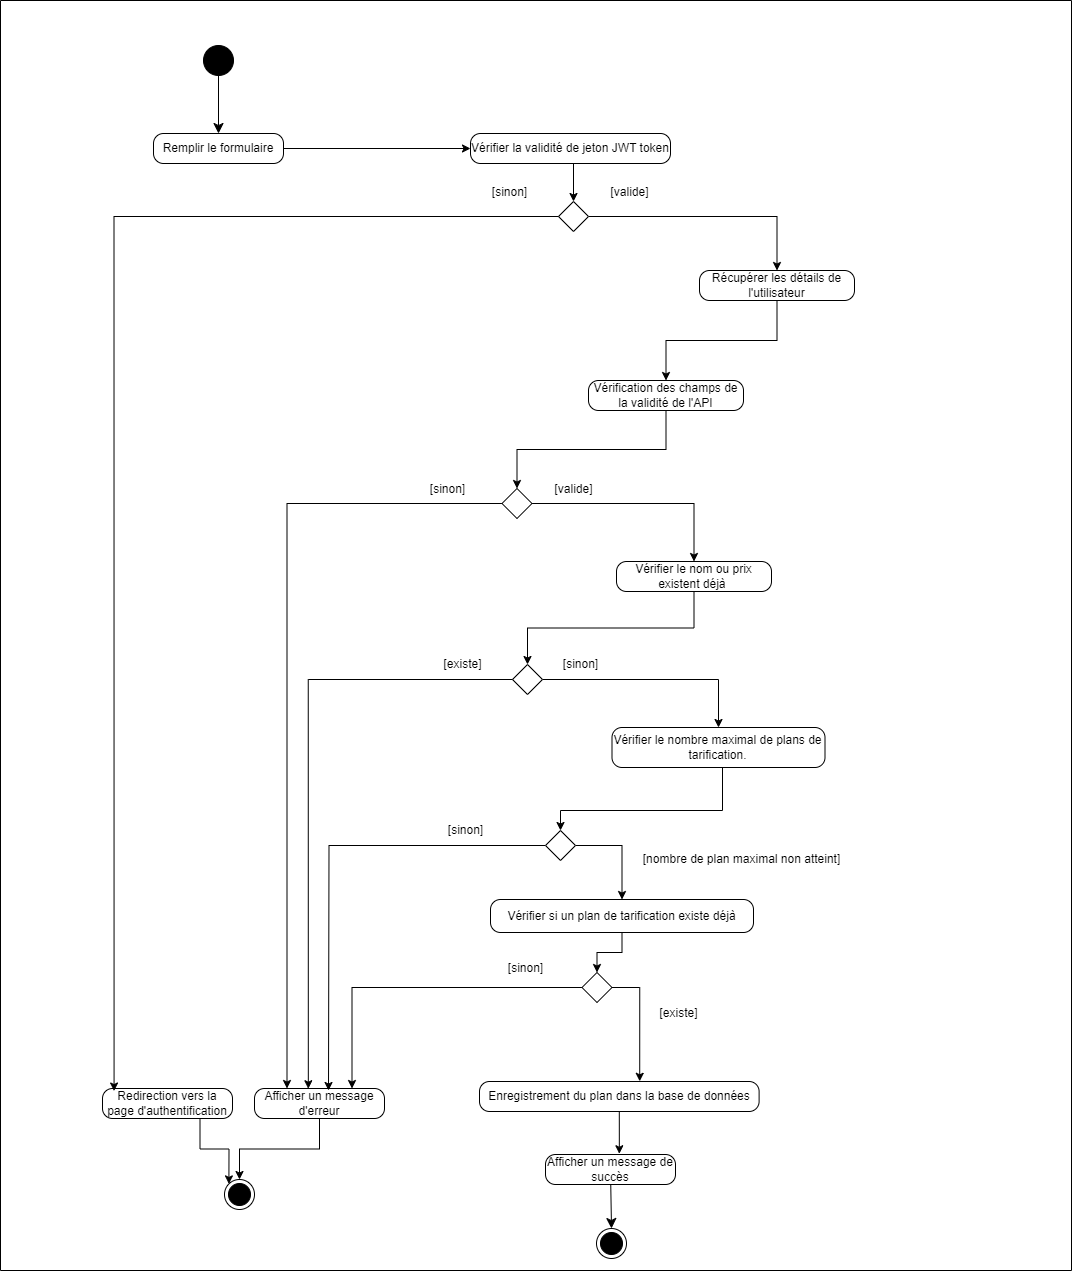
\includegraphics[width=1.1\columnwidth]{diagrammedactiviteAjouterPlandetarification.png}}
    \caption{Diagramme d'activités "Ajouter Plan de tarification"}
    \label{fig:logo_tt}
\end{figure}
\pagebreak

\subsection{Diagramme d'activités "Consommer une API "}
Ce diagramme d'activités décrit le processus de consommation d'une API. Tout commence lorsque le développeur envoie une demande de consommation. Le système vérifie d'abord la validité de la clé de l'utilisateur. Si elle est invalide, un message d'erreur est retourné. \\
Sinon, le système vérifie si l'API spécifiée existe. Si elle n'existe pas, un message d'erreur est retourné. Ensuite, la validité de la souscription est vérifiée. En cas de souscription invalide, une erreur est signalée. \\
Sinon, le système vérifie si l'endpoint spécifié existe. S'il n'existe pas, une erreur est retournée. Ensuite, le système crée une requête HTTP, y ajoute l’entête de  l'API, puis envoie la requête au fournisseur de services API. En cas de serveur hors service, un message d'erreur est affiché. \\
Si le serveur répond, le système enregistre la réponse et met à jour le crédit de l'utilisateur.
\begin{figure}[H]
    \centering
    \frame{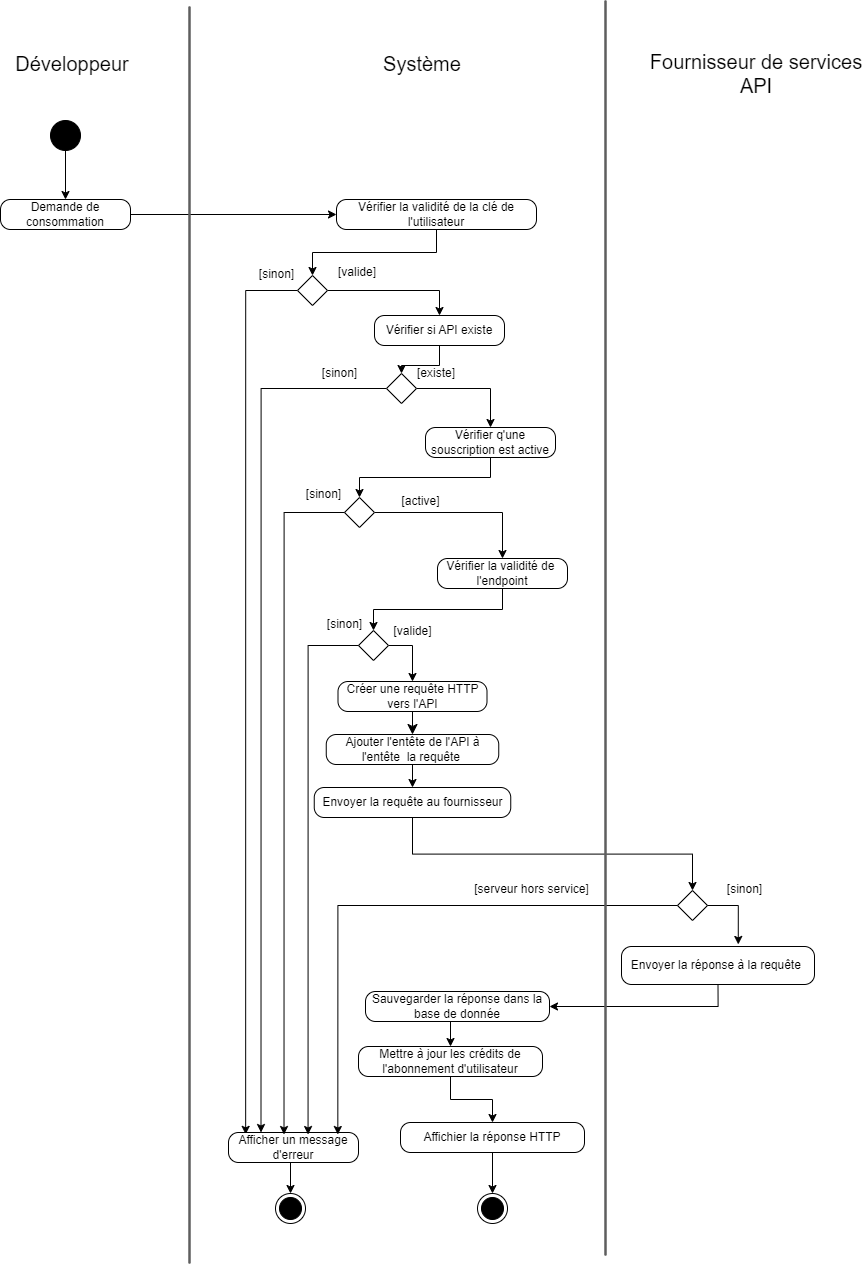
\includegraphics[width=1\columnwidth]{diagrammedactiviterconsommation.png}}
    \caption{Diagramme d'activités "Consommer une API "}
    \label{fig:logo_tt}
\end{figure}
\pagebreak

\subsection{Diagramme de séquence "Consommer une API"}
Ce diagramme de séquence illustre la séquence d'interactions entre les différents composants pour réaliser la consommation d’une API en dehors de la marketplace. Le processus commence lorsque le développeur exécute une requête. \\ 
Le middleware d'authentification vérifie si la clé existe dans la base de données. Si la clé n'existe pas, un message d’erreur est retourné. Sinon, le middleware API vérifie si l'API est valide. Si l'API est invalide, un message d’erreur est retourné. \\ 
Sinon, le middleware de souscription vérifie si la souscription est active. Si la souscription n'est pas valide, un message d'erreur est retourné .Sinon le contrôleur de consommation vérifie si le endpoint existe. S'il n'existe pas, un message d’erreur est retourné. \\
Sinon il  crée une requête HTTP, y ajoute l’en-tête de l'API, puis envoie la requête au fournisseur. La réponse est ensuite enregistrée au niveau de la classe request. En cas de serveur hors service, un message d'erreur est affiché. Sinon, le crédit de l'utilisateur est mis à jour et la réponse est affichée.
\begin{figure}[H]
    \centering
    \frame{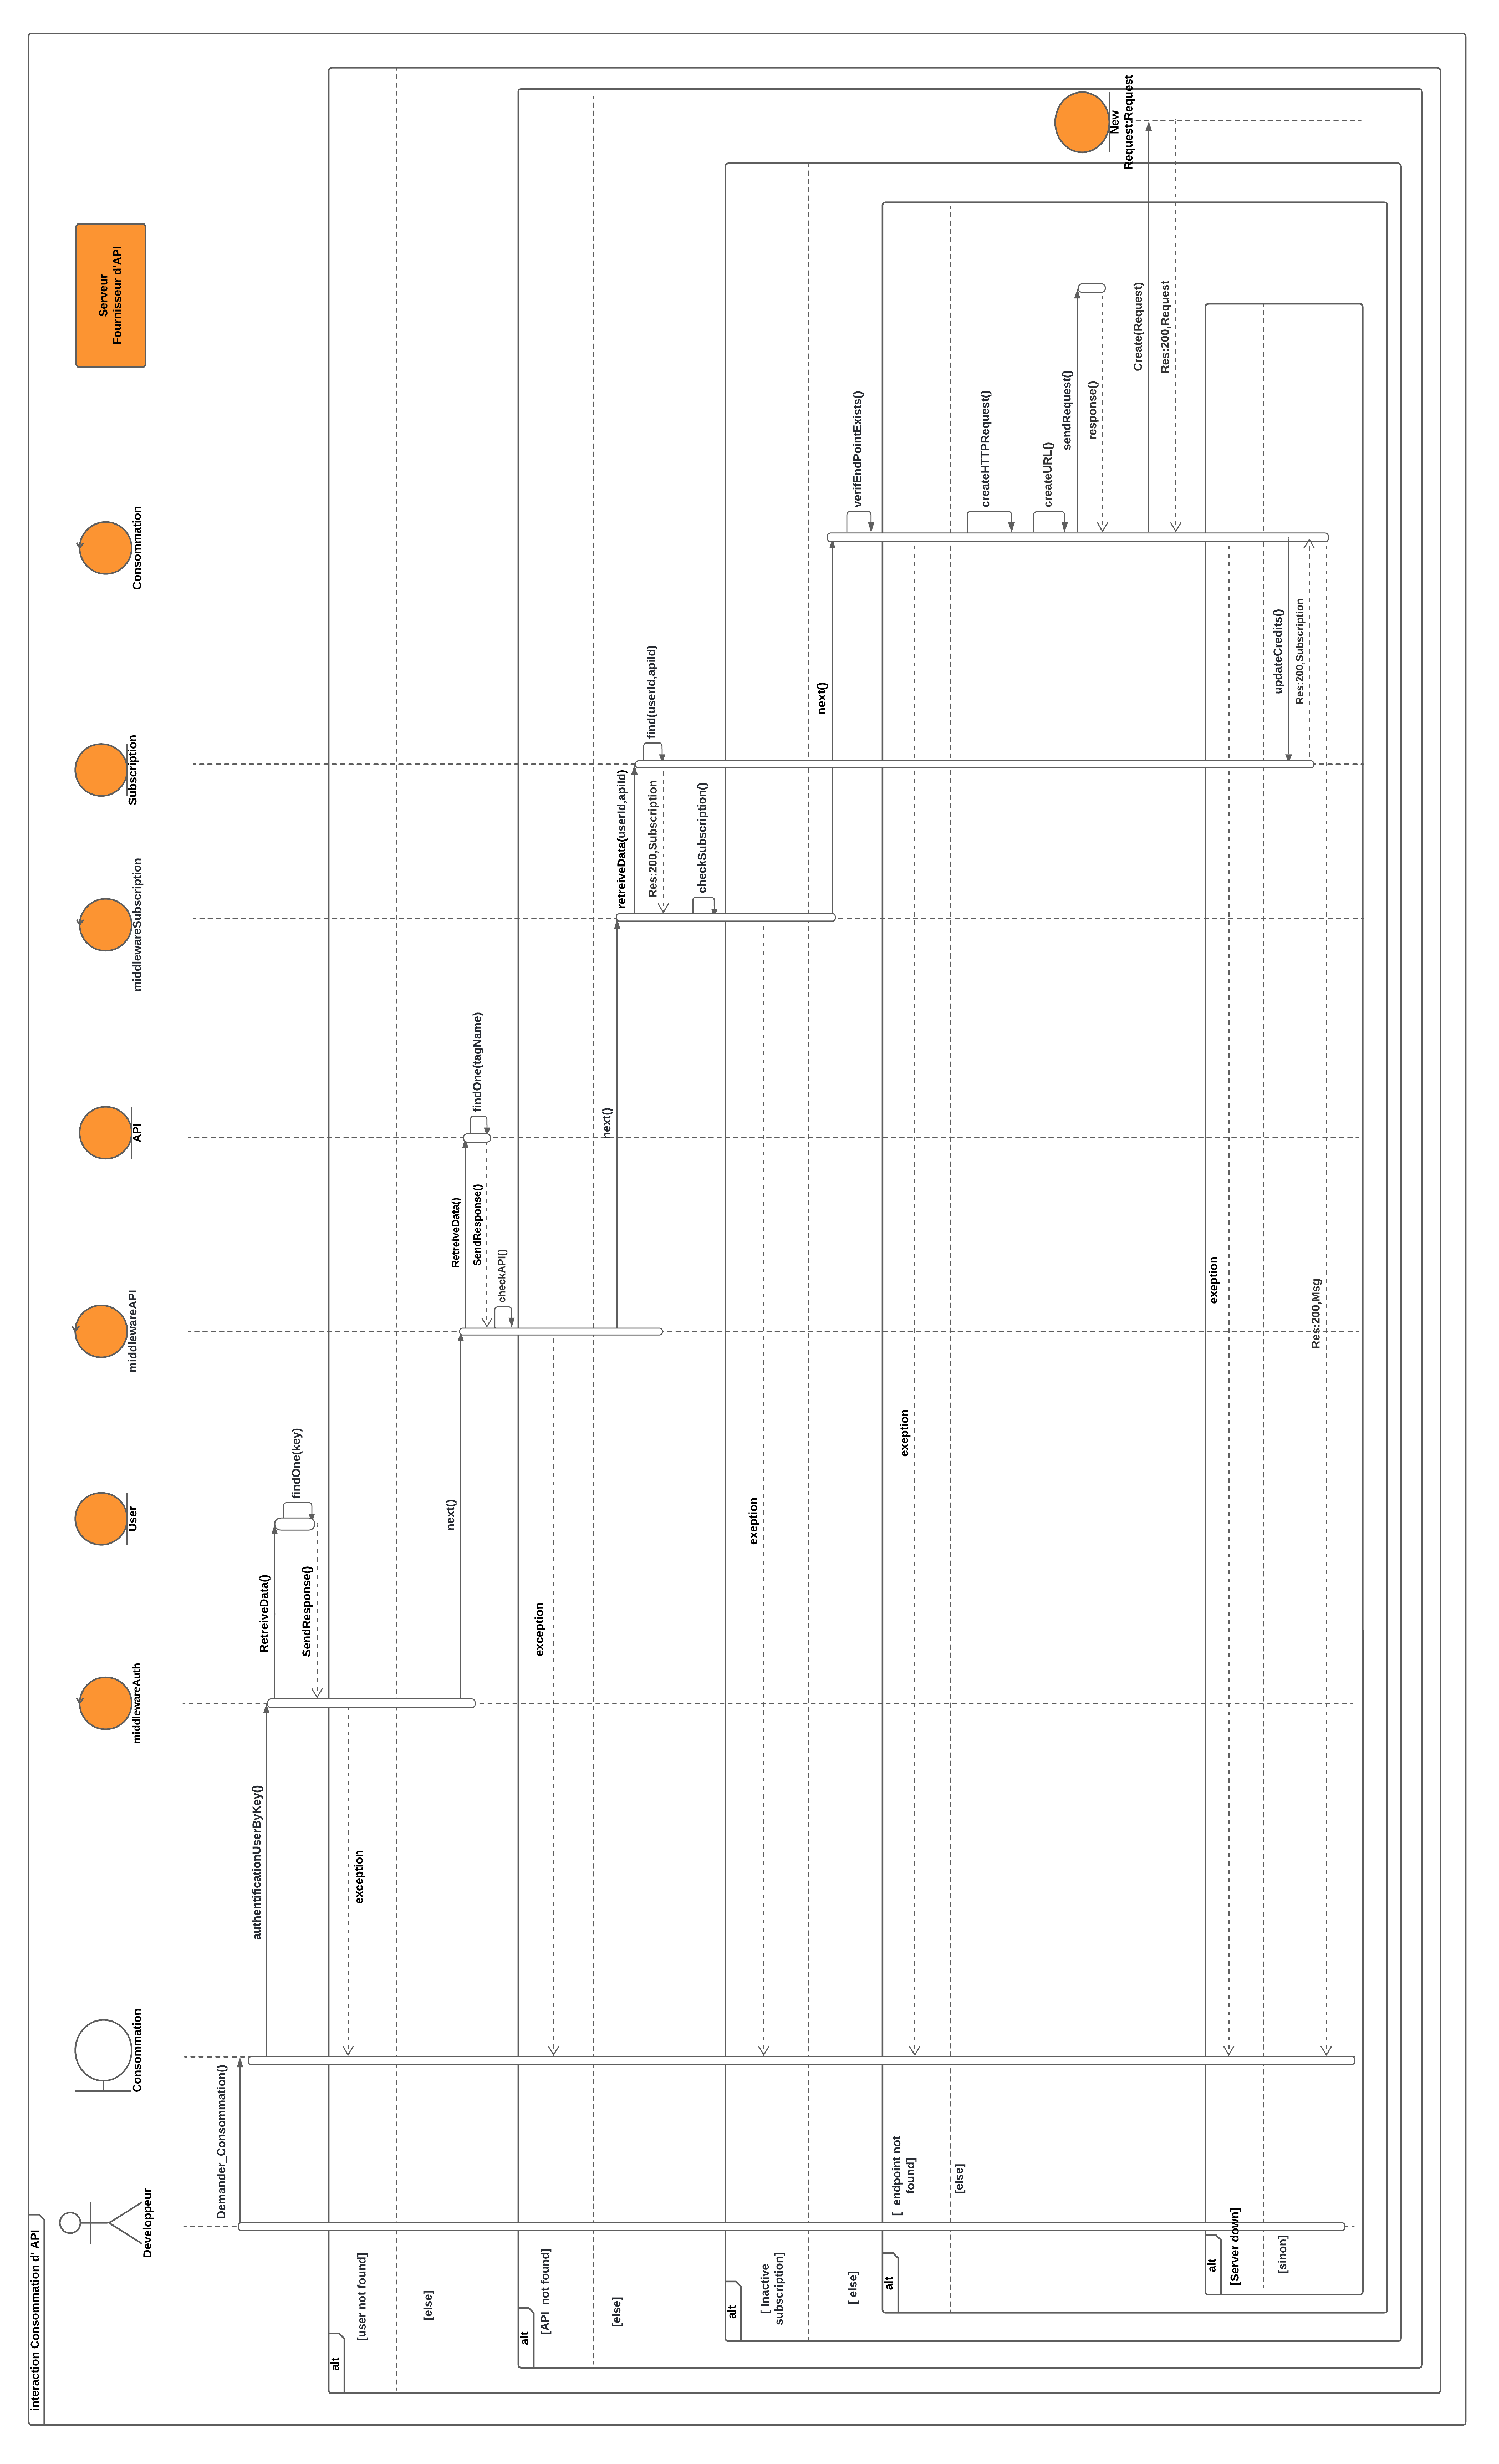
\includegraphics[width=0.9\columnwidth]{DiagrammeDeSequenceConsommation .png    }}
    \caption{Diagramme de séquence "Consommer une API"}
    \label{fig:logo_tt}
\end{figure}
\pagebreak

\subsection{Diagramme d'activités de "Souscription à une API"} 
Ce diagramme d’activités décrit le processus de souscription à une API. Tout commence lorsque le développeur envoie une demande de souscription. Le système vérifie d’abord la validité du jeton JWT. Si le jeton est invalide, un message d’erreur est retourné.  Sinon, le système récupère les détails de l'utilisateur et vérifie s'il possède déjà une souscription active. Si une souscription existe, un message d’erreur est retourné.\\
Ensuite, le système crée une nouvelle souscription. Si l'API est gratuite, la souscription est activée immédiatement et un message de succès est affiché. Si l'API est payante, le système crée un paiement en attente. \\
Stripe intervient alors pour créer une session de vérification de paiement et redirige vers l'URL de prise de la session. Stripe traite le paiement. En cas d'échec du paiement, il demande de réintroduire les données de paiement. Si le paiement est réussi, le système met à jour le statut de paiement, active la souscription et affiche un message de succès, puis redirige le développeur vers l'URL de succès. \\
\begin{figure}[H]
    \centering
    \frame{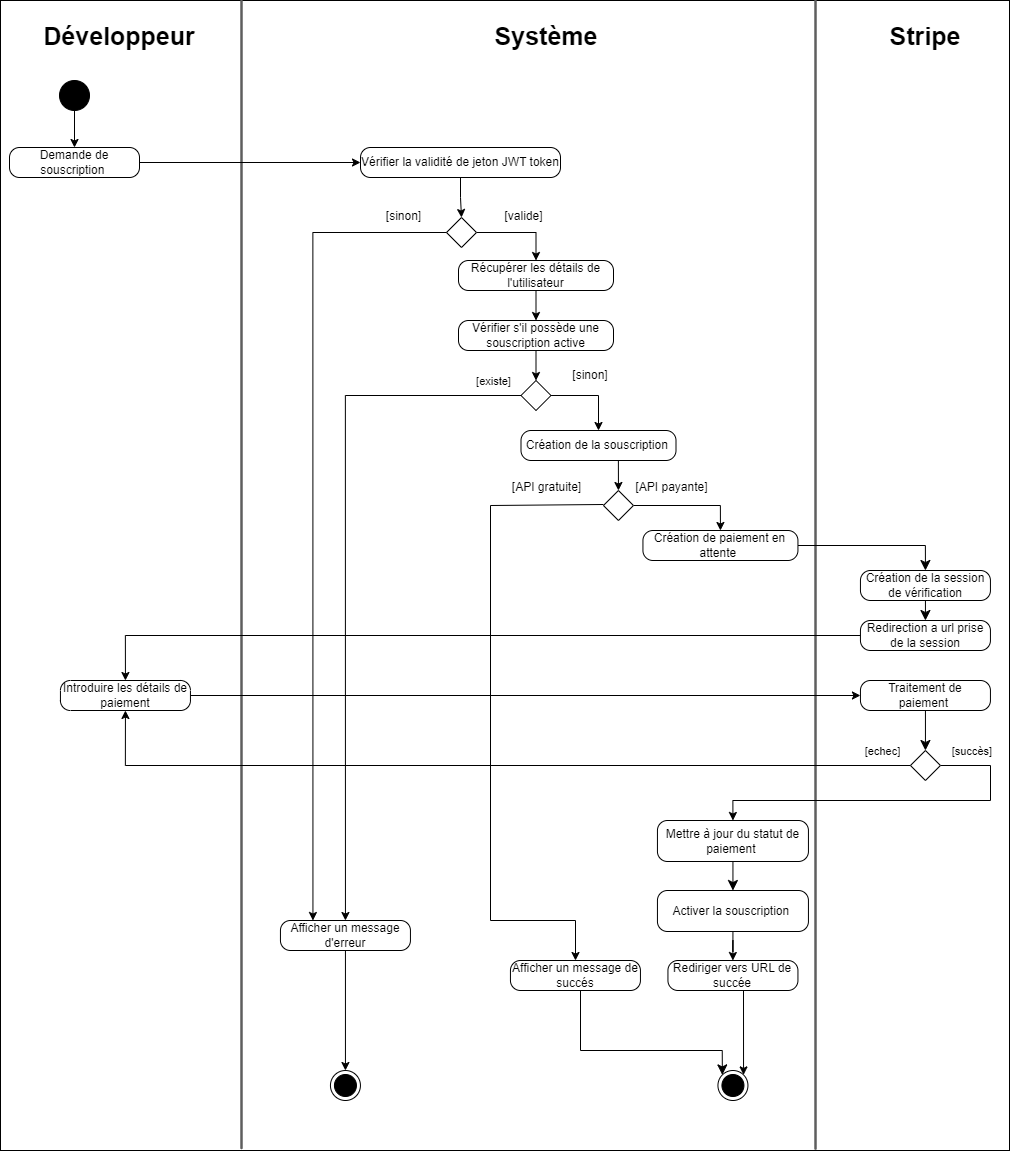
\includegraphics[width=1.1\columnwidth]{Diagrammedactivitedepaiement.png}}
    \caption{Diagramme d'activités "Souscription à une API" }
    \label{fig:logo_tt}
\end{figure}
\pagebreak

\section{Revue de sprint}
Dans cette partie, nous allons exposer le travail réalisé durant le sprint 2, ainsi que le burndown chart.
    \subsection{Réalisation}
    Dans cette étape, nous allons explorer les interfaces réalisées lors de ce sprint.
   
    \subsubsection{Gestion de la tarification}
    Cette interface représente le formulaire d'ajout d'un plan de tarification
    \begin{figure}[H]
        \centering
        \frame{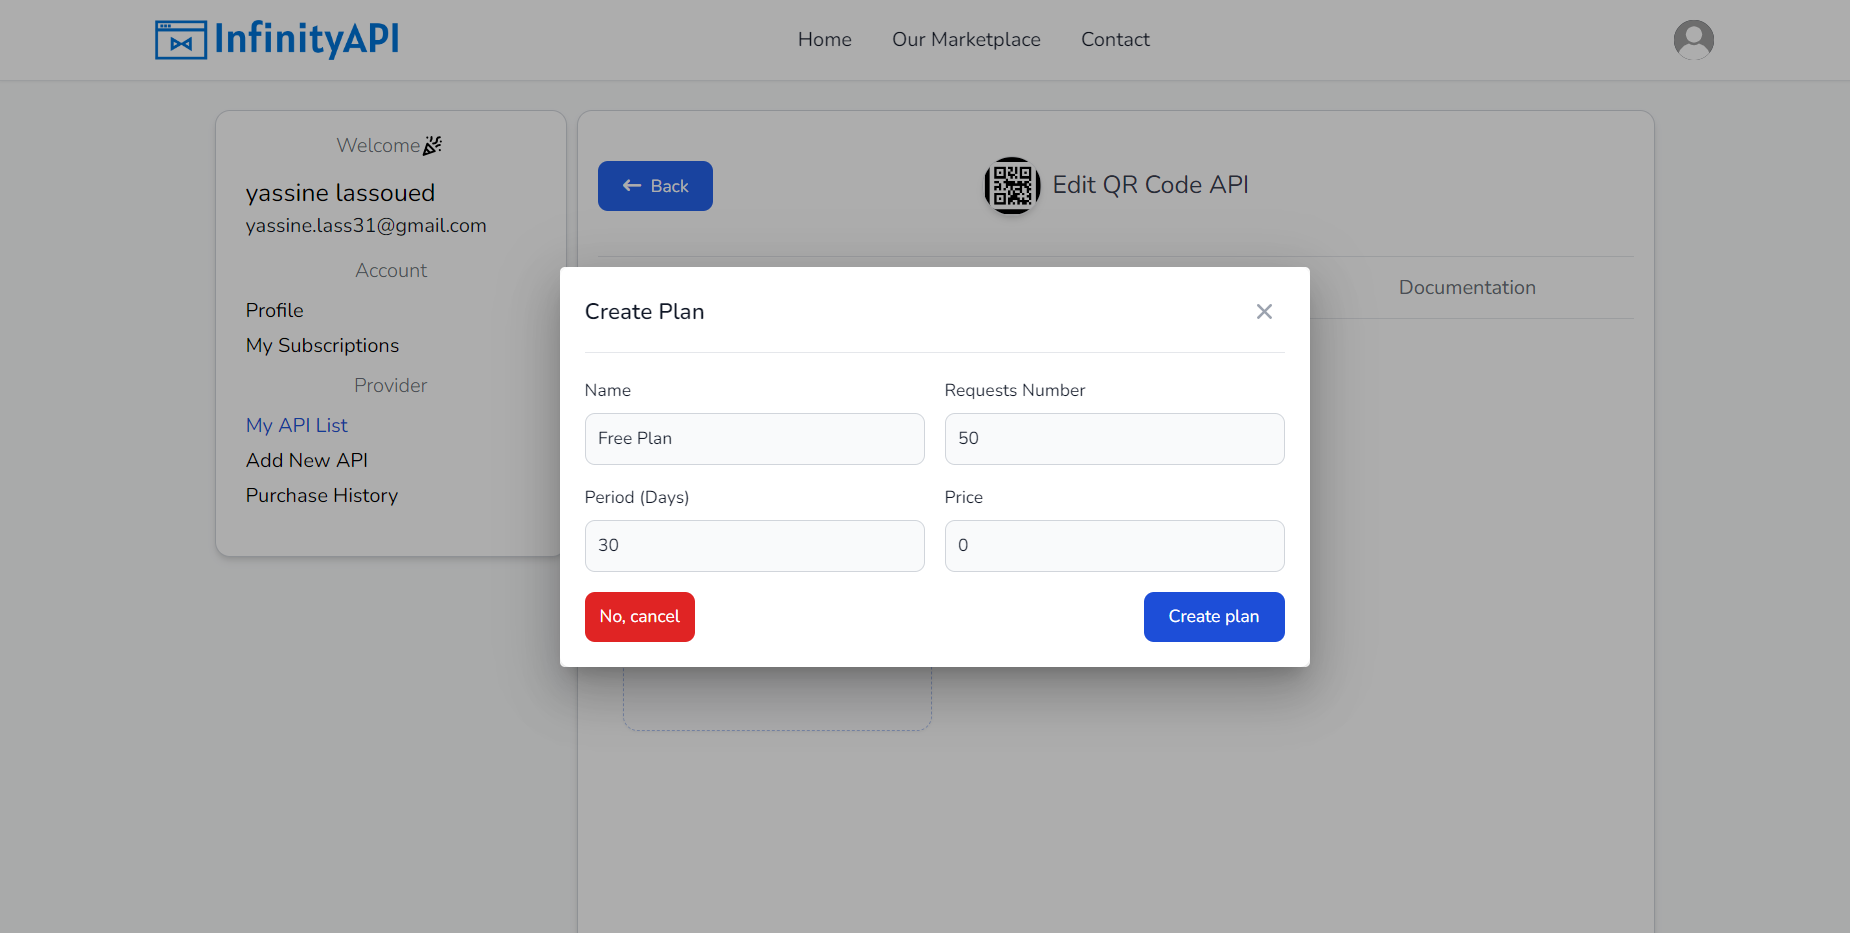
\includegraphics[width=0.7\columnwidth]{Interfacedajoutdeplandetarification.png}}
        \caption{ Interface d'ajout de plan de tarification }
        \label{fig:logo_tt}
    \end{figure}

    Après avoir rempli le formulaire, l'utilisateur peut consulter les plans de tarification ajoutés, et il peut cliquer sur "Créer un nouveau plan" à condition que le nombre de plans ne dépasse pas 4. 
    \begin{figure}[H]
        \centering
        \frame{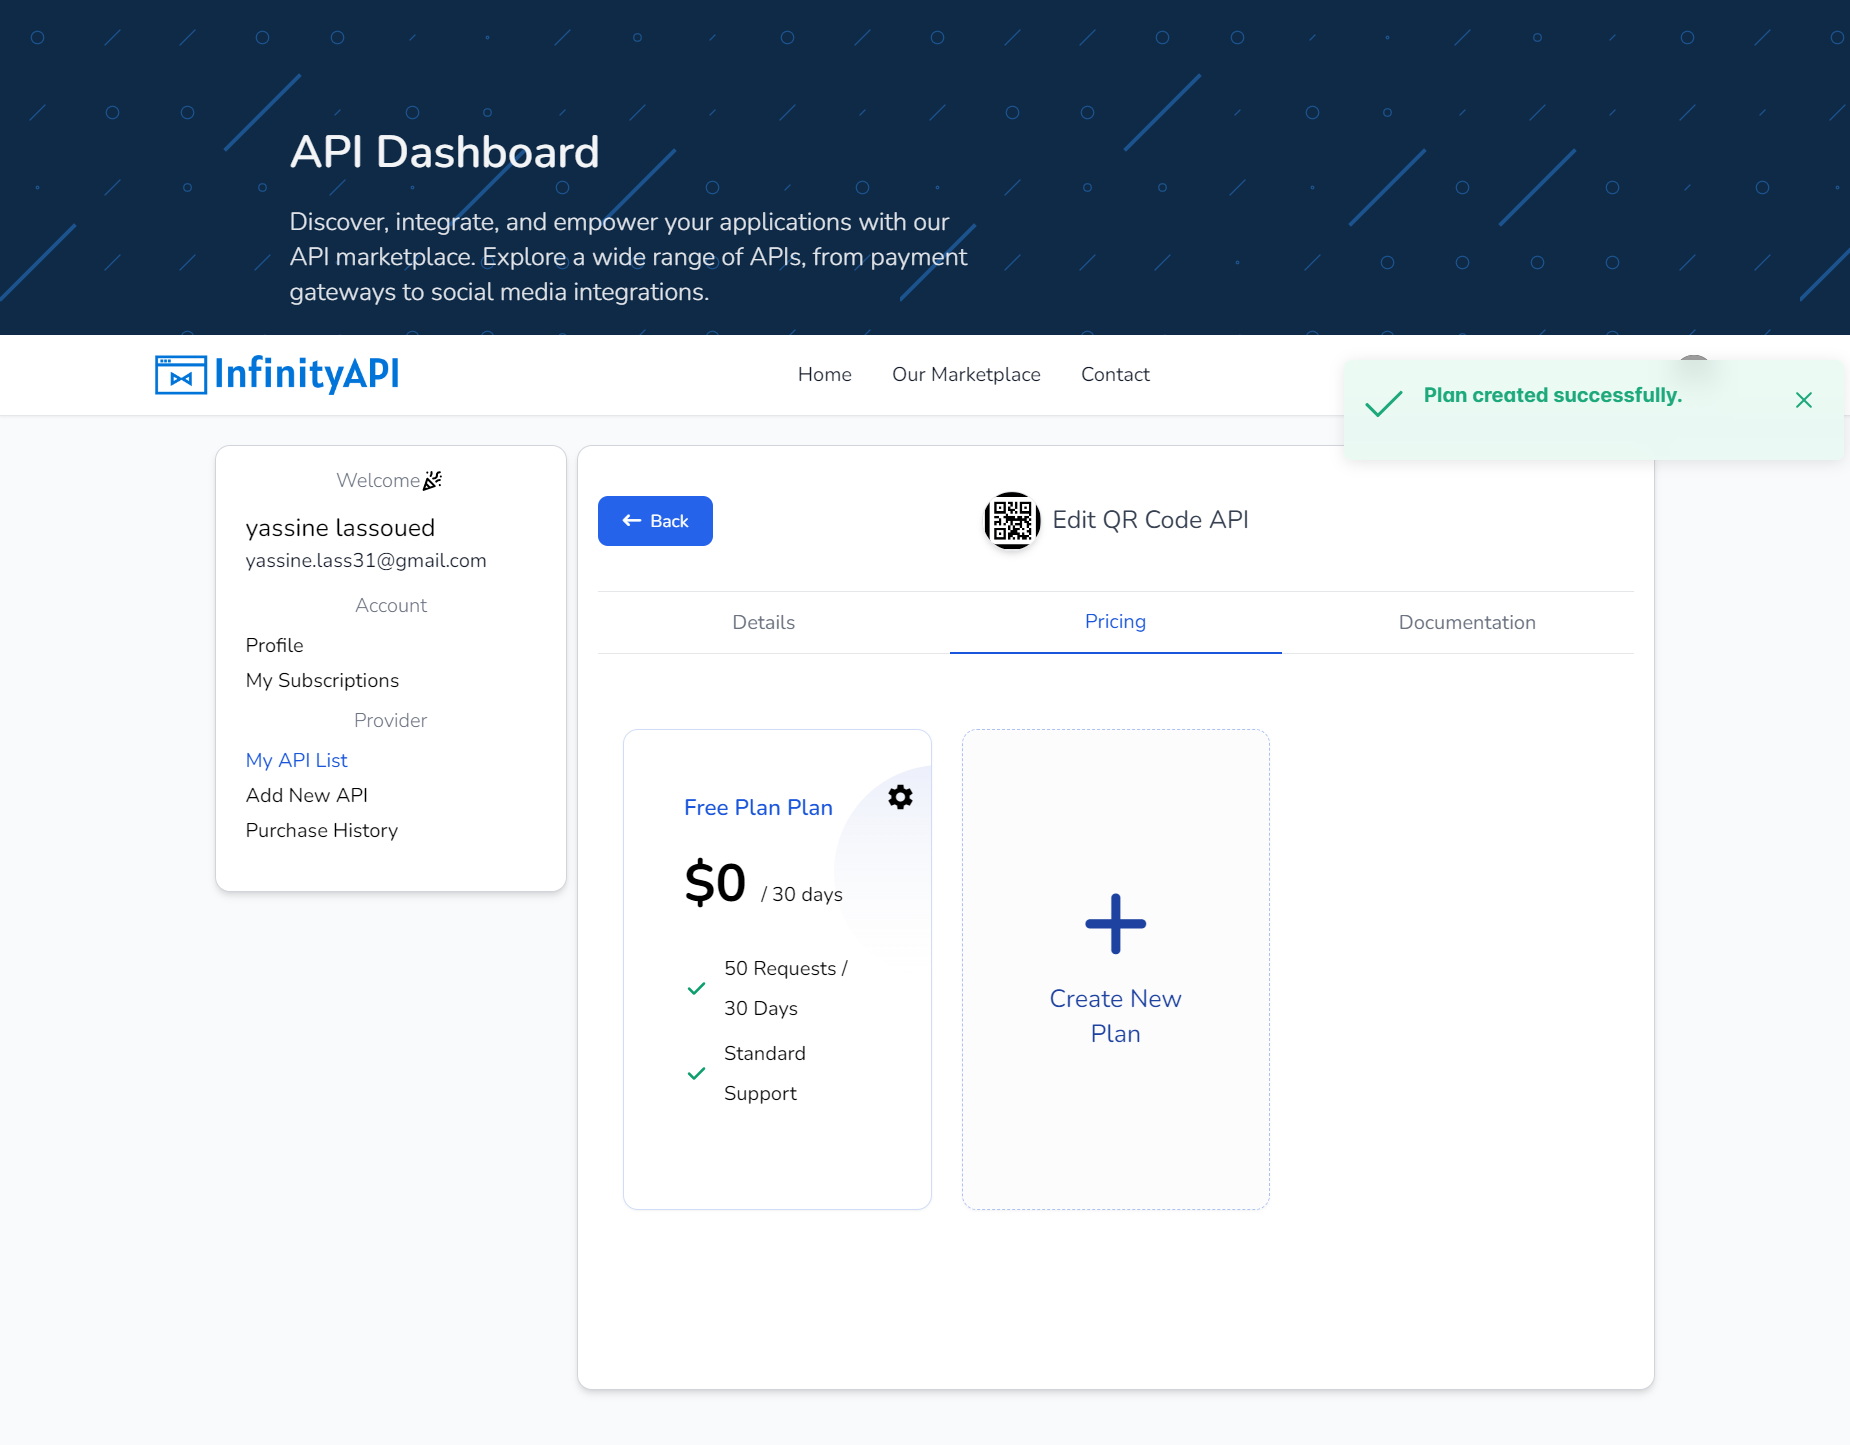
\includegraphics[width=0.6\columnwidth]{Interfacedelistedesplansdetarification.png}}
        \caption{ Interface de la liste des plans de tarification }
        \label{fig:logo_tt}
    \end{figure}

    \subsubsection{Souscription à une API }
    Cette interface représente le processus de souscription pour une API payante.
    \begin{figure}[H]
        \centering
        \frame{\includegraphics[width=1.1\columnwidth]{InterfacedeenchaînementdelasouscriptionauneAPI.png}}
        \caption{Interface de l'enchaînement de la souscription à une API }
        \label{fig:logo_tt}
    \end{figure}
    \pagebreak
    \subsubsection{Test d'API}
    Cette interface représente l'interface de test d'API dans notre plateforme.
    \begin{figure}[H]
        \centering
        \frame{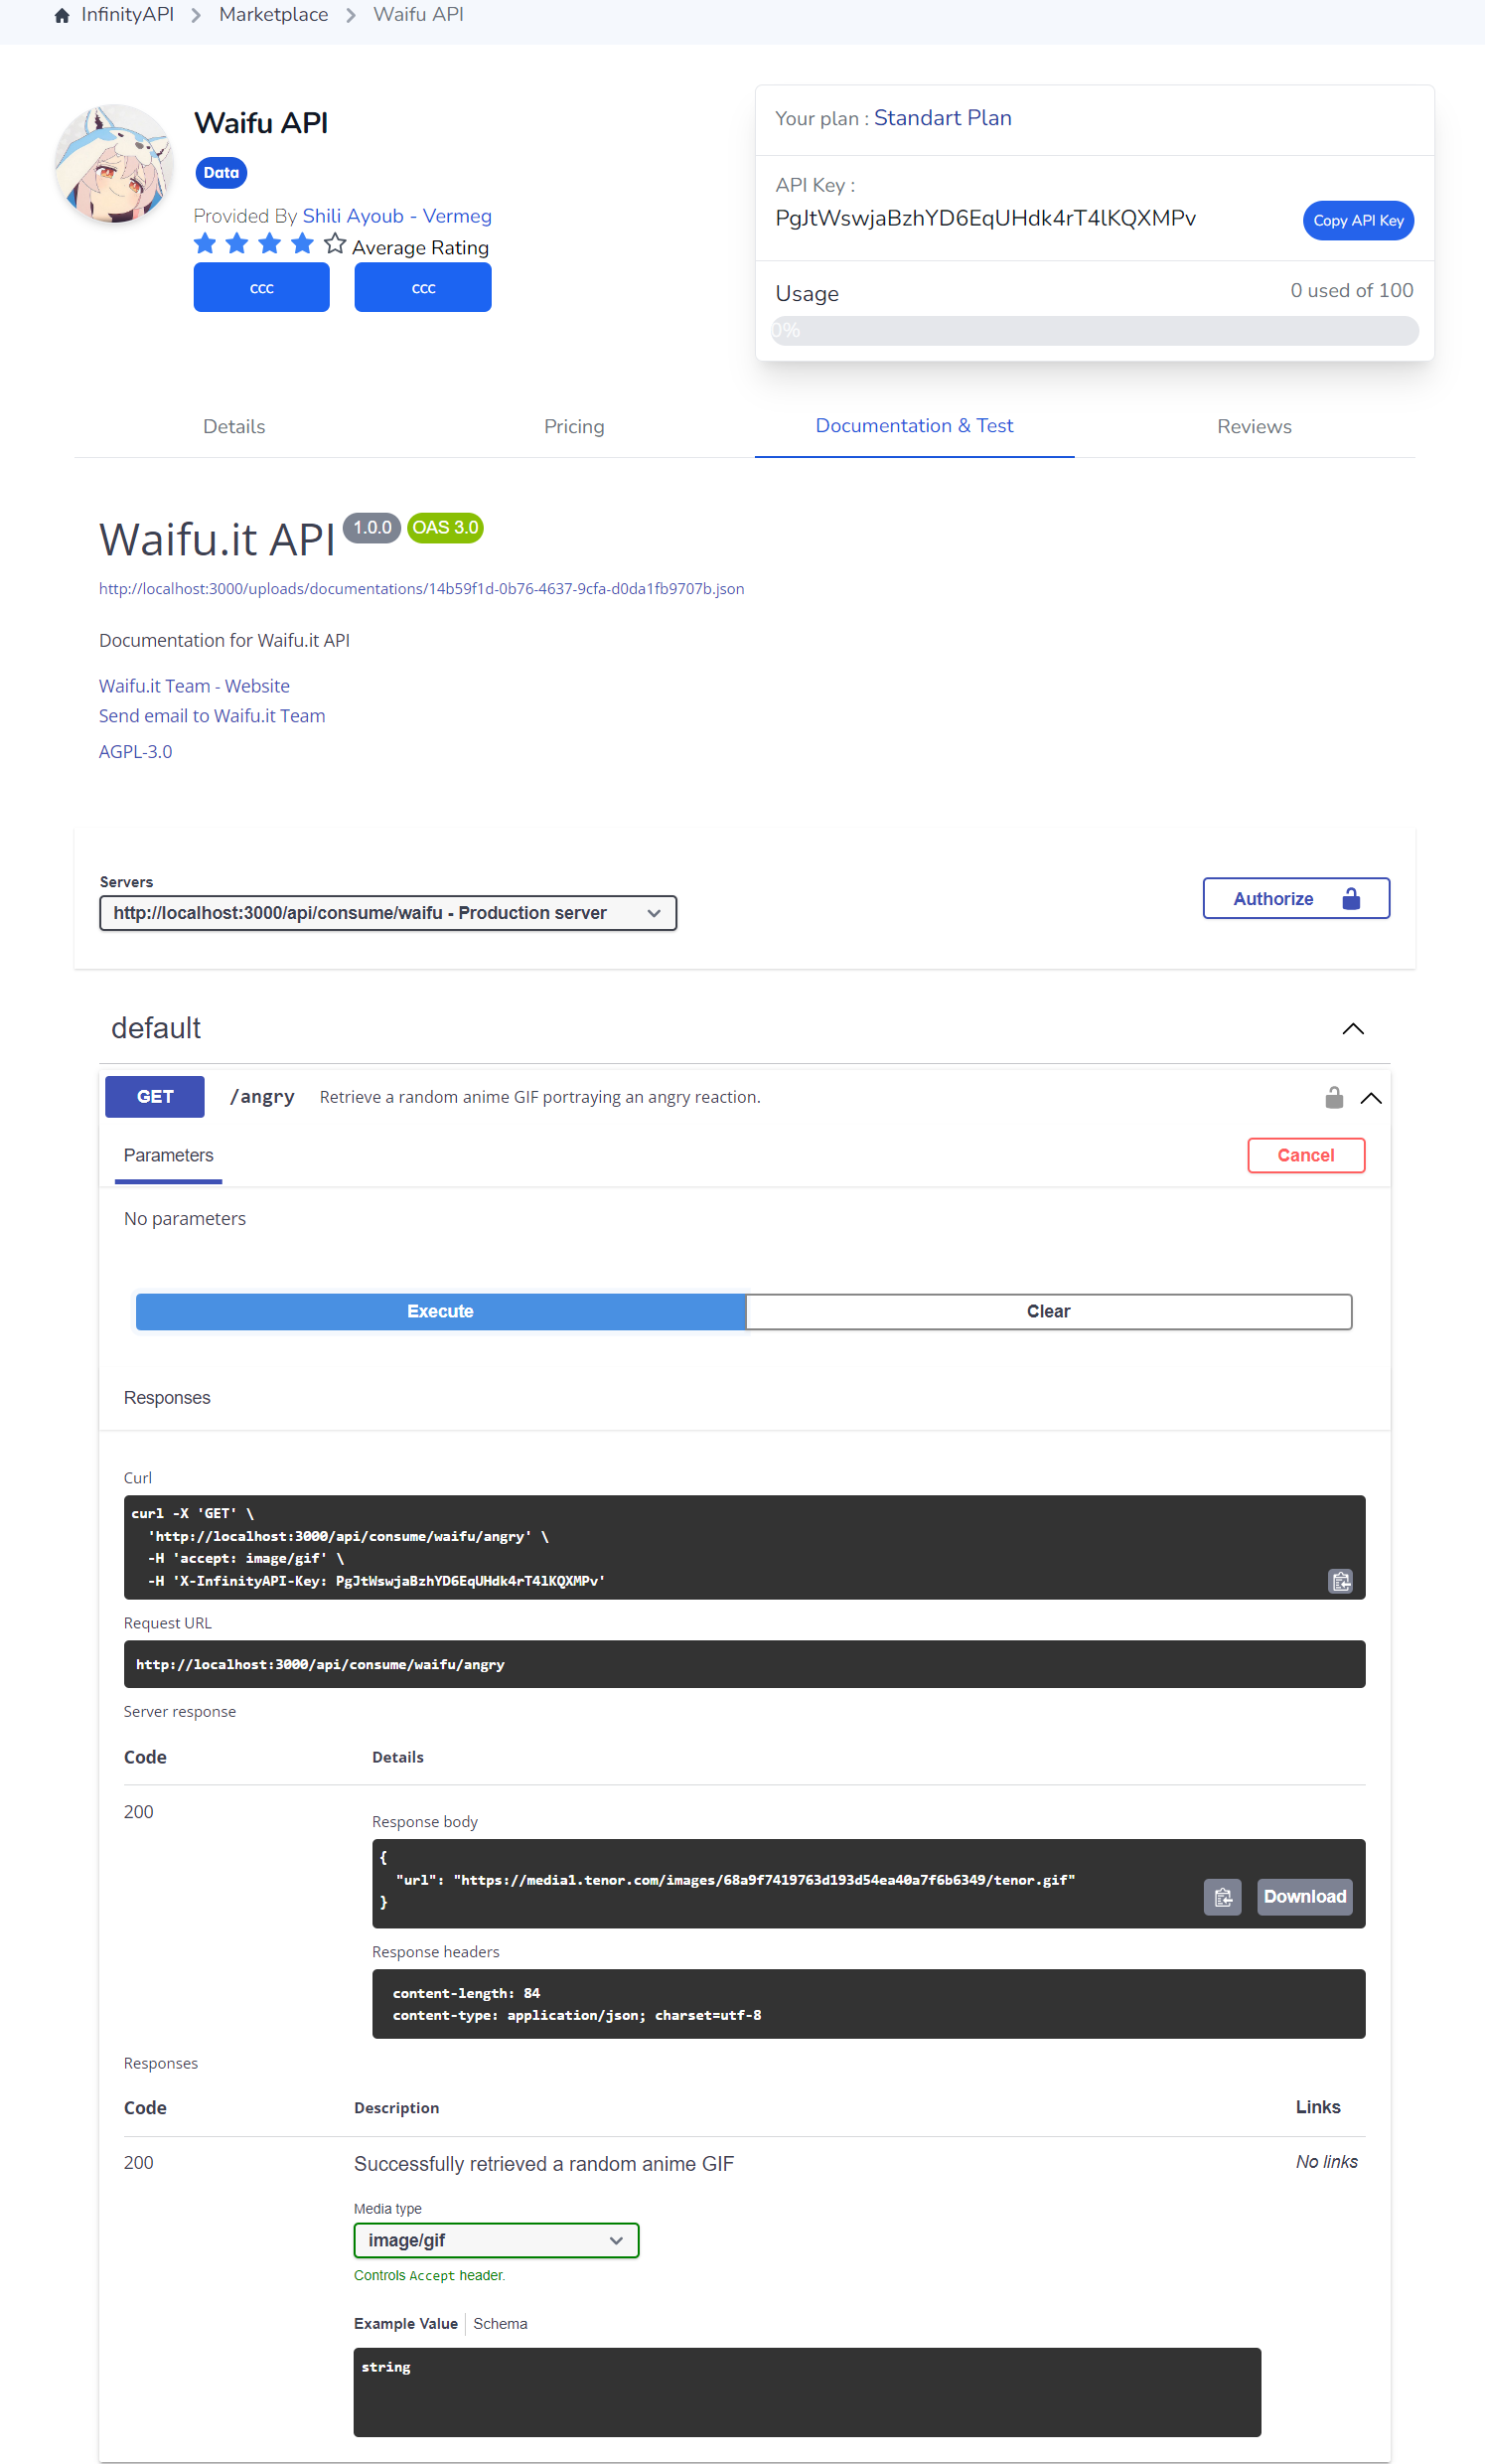
\includegraphics[width=0.8\columnwidth]{testAPI.png}}
        \caption{Interface de test d'une API}
        \label{fig:logo_tt}
    \end{figure}
    
    \subsubsection{Dashboard administrateur}
    Cette interface présente la liste des développeurs qui utilisent notre marketplace.       
        \begin{figure}[H]    
        \centering
            \frame{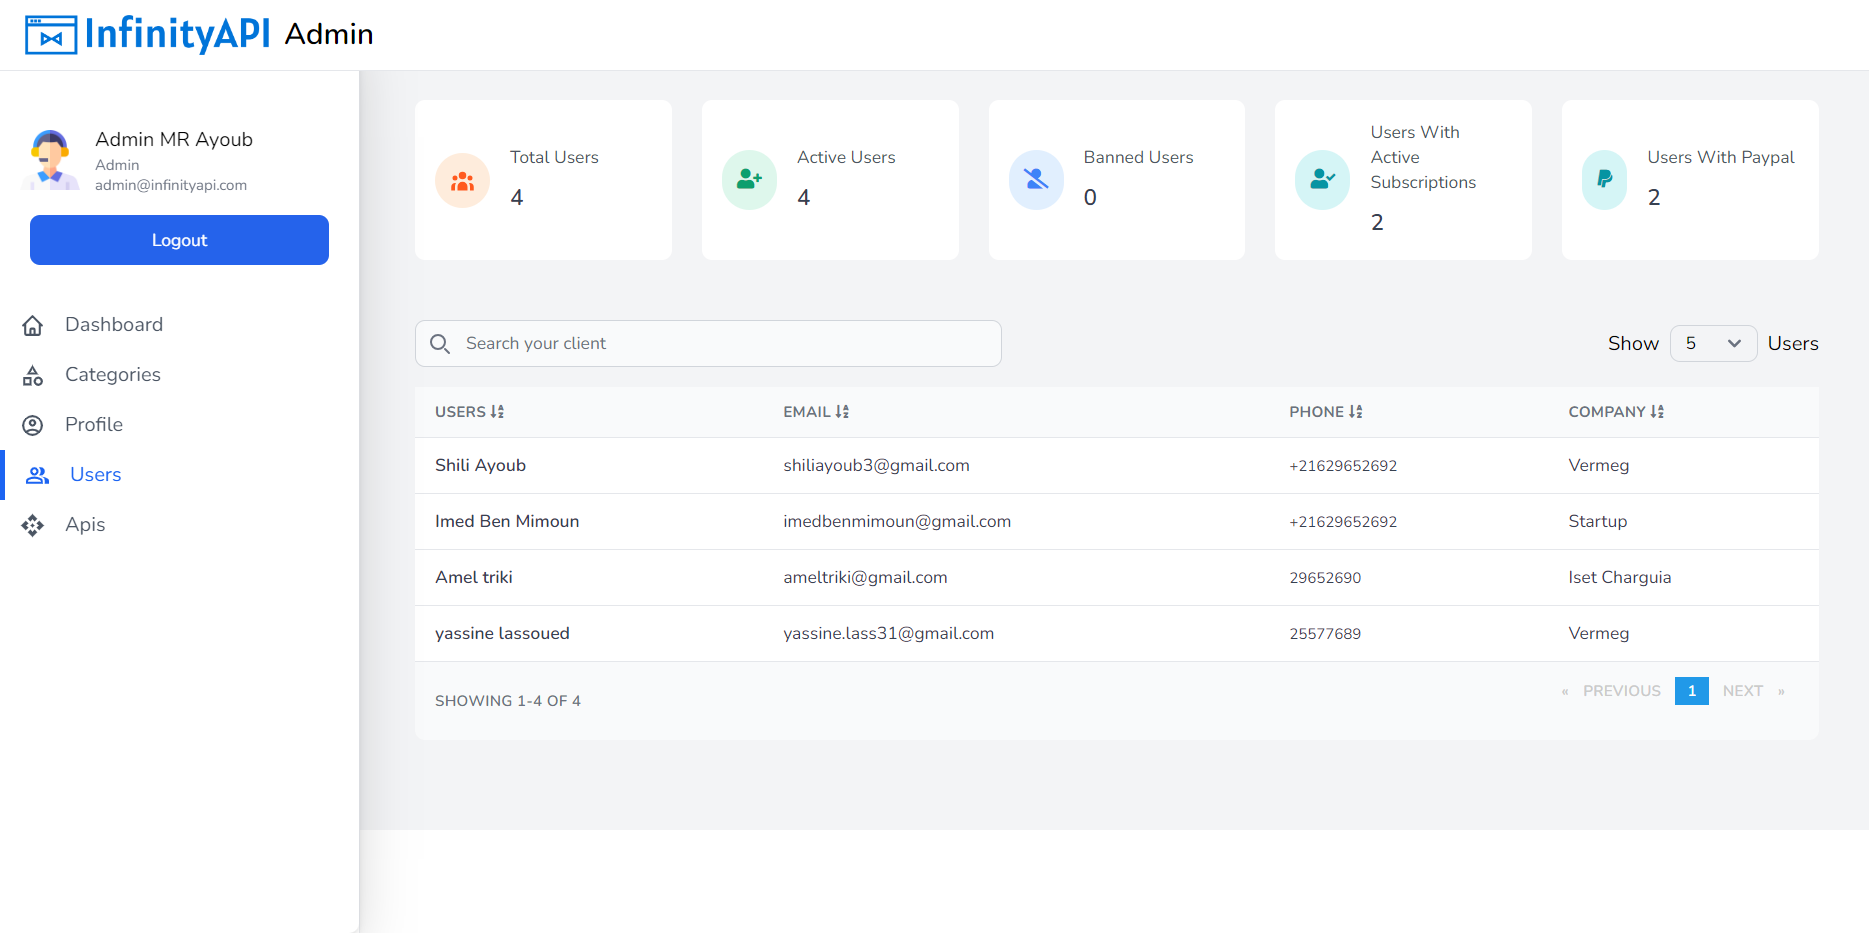
\includegraphics[width=1\columnwidth]{ListeUsers.png}}
            \caption{Interface de la liste des développeurs }
            \label{fig:logo_tt}
        \end{figure}

        Cette interface permet de gérer le profil d'un utilisateur, notamment en lui permettant de bloquer et de débloquer un utilisateur.
        \begin{figure}[H]    
        \centering
            \frame{\includegraphics[width=1\columnwidth]{ Interfacedeprofildéveloppeur.png     }}
            \caption{Interface de profil développeur }
            \label{fig:logo_tt}
        \end{figure}


        \subsection{Burndown Chart}
        \begin{figure}[H]    
            \centering
                \frame{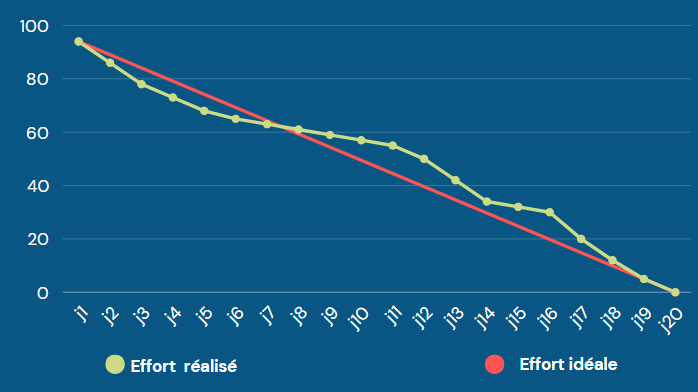
\includegraphics[width=0.9\columnwidth]{ Burndown_Chart_du_sprint2.png     }}
                \caption{Burndown chart du sprint 2}
                \label{fig:logo_tt}
            \end{figure} 
            Ce burndown montre que :
            \begin{itemize}
                \item Tous les user stories sont réalisés dans le temps estimé.
                \item La vélocité de notre équipe est 94
            \end{itemize}
            
            \subsection{Rétrospective du sprint 2}
            \begin{longtable}[c]{|p{0.25\linewidth}|p{0.7\linewidth}|}
                \hline
                \textbf{Les questions} & \textbf{Les réponses} \\
                \hline
                \endfirsthead
                \multicolumn{2}{c}%
                {{\bfseries \tablename\ \thetable{} -- suite de la page précédente}} \\
                \hline
                \textbf{Les questions} & \textbf{Les réponses} \\
                \hline
                \endhead
                \hline \multicolumn{2}{|r|}{{\bfseries Suite à la page suivante}} \\
                \hline
                \endfoot
                \hline
                \endlastfoot
            
                \multirow{3}{=}{Ce qui s'est bien passé} & Maîtrise de l'intégration de l'API Stripe \\
                & Avancement des fonctionnalités clés\\
                &Collaboration efficace \\
                \hline
                \multirow{2}{=}{Les problèmes rencontrés} & Déséquilibre dans le temps de travail pendant le mois de Ramadan \\
                & Problèmes d'intégration\\
                \hline
                \multirow{1}{=}{Les choses à améliorer} &Tests plus rigoureux \\
                \hline
            \end{longtable}

\section*{Conclusion}
Tout au long de ce chapitre, nous avons présenté le travail effectué au niveau du deuxième sprint, en termes de spécification, conception et réalisation. Dans le chapitre suivant, nous aborderons le dernier sprint.
        \clearpage
        
        \chapter{Sprint 3 "Demande de payout, statistiques et signalement d'erreurs"}

\section*{Introduction}
Dans ce chapitre, nous examinerons le dernier sprint, qui suit les mêmes étapes que le précédent. Nous débuterons par un extrait du backlog du sprint 3, puis passerons aux spécifications fonctionnelles, à la conception, à la revue du sprint, et conclurons par une rétrospective.

\section{ Extrait du backlog du sprint 3}
Les thèmes du sprint sont : La gestion des demandes de payout, dashboard statistique, le système de notifications, ainsi que la gestion des signalements d'erreurs et des feedbacks. \\
Nous allons maintenant présenter un extrait du sprint backlog à travers le user story : "En tant que développeur, je veux pouvoir consulter les statistiques de consommation de mes APIs "

\begin{table}[H]
    \centering
    \caption{Extrait du backlog du sprint3 "Statistiques de consommation de mes API"}
    \label{tab:task_estimation_statistics}
    \begin{longtable}{|p{0.25\linewidth}|p{0.25\linewidth}|p{0.35\linewidth}|p{0.15\linewidth}|}
        \hline
        \textbf{User story} & \textbf{Tâches} & \textbf{Sous-tâches} & \textbf{Estimation} \\
        \hline
        \endfirsthead
        \multicolumn{4}{c}%
        {{\bfseries \tablename\ \thetable{} -- suite de la page précédente}} \\
        \hline
        \textbf{User story} & \textbf{Tâches} & \textbf{Sous-tâches} & \textbf{Estimation} \\
        \hline
        \endhead
        \hline \multicolumn{4}{|r|}{{\bfseries Suite à la page suivante}} \\
        \hline
        \endfoot
        \hline
        \endlastfoot

        \multirow{8}{=}{En tant que développeur, je veux pouvoir consulter les statistiques de consommation de mes APIs.}
            & Préparation de la maquette & Réalisation de la maquette & 2h \\
        \cline{2-4}
            & \multirow{1}{=}{Modélisation \& conception UML} & Réalisation du diagramme de séquence & 2h \\
        \cline{2-4}
            & \multirow{2}{=}{Préparation du backend} & Réalisation de la fonction get "getConsumerAnalytics" & 3h \\
        \cline{3-4}
            & & Test & 2h \\
        \cline{2-4}
            & \multirow{4}{=}{Préparation du frontend} & Réalisation de l'interface & 2h \\
        \cline{3-4}
            & & Préparation du service "StatisticService" & 1h 30min \\
        \cline{3-4}
            & & Préparation de la fonction “createConsumerLineChart” & 1h 30min \\
        \cline{3-4}
            & & Test & 30min \\
        \hline
    \end{longtable}
\end{table}

\pagebreak

\section{ Spécification fonctionnelle}
Dans cette partie, nous allons présenter le diagramme de cas d'utilisation du sprint 3 et un exemple de maquette.

\subsection{Diagramme de cas d'utilisation}
Dans cette partie, nous allons présenter le diagramme de cas d'utilisation du sprint 3. \\
Les cas d'utilisation suivants ont été intégrés au sprint 3.

\begin{itemize}
    \item  \textbf{Développeur}
    \begin{itemize}
        \item  Consulter mes statistiques.
        \item Consulter mes transactions.
        \item Gérer mes feedbacks.
        \item Consulter mes notifications.
        \item Gérer les signalements.
    \end{itemize}
    \item  \textbf{Administrateur}
    \begin{itemize}
        \item Gérer les demandes de payout.
        \item Consulter les statistiques.
        \item Consulter les signalements.
        \item Consulter mes notifications.
    \end{itemize} 
   
\end{itemize}
Un acteur secondaire a été introduit au niveau de ce sprint :
\begin{itemize}
\item \textbf{Paypal} pour la réalisation du payout.
\end{itemize} 
\pagebreak


\begin{figure}[H]
    \centering
    \frame{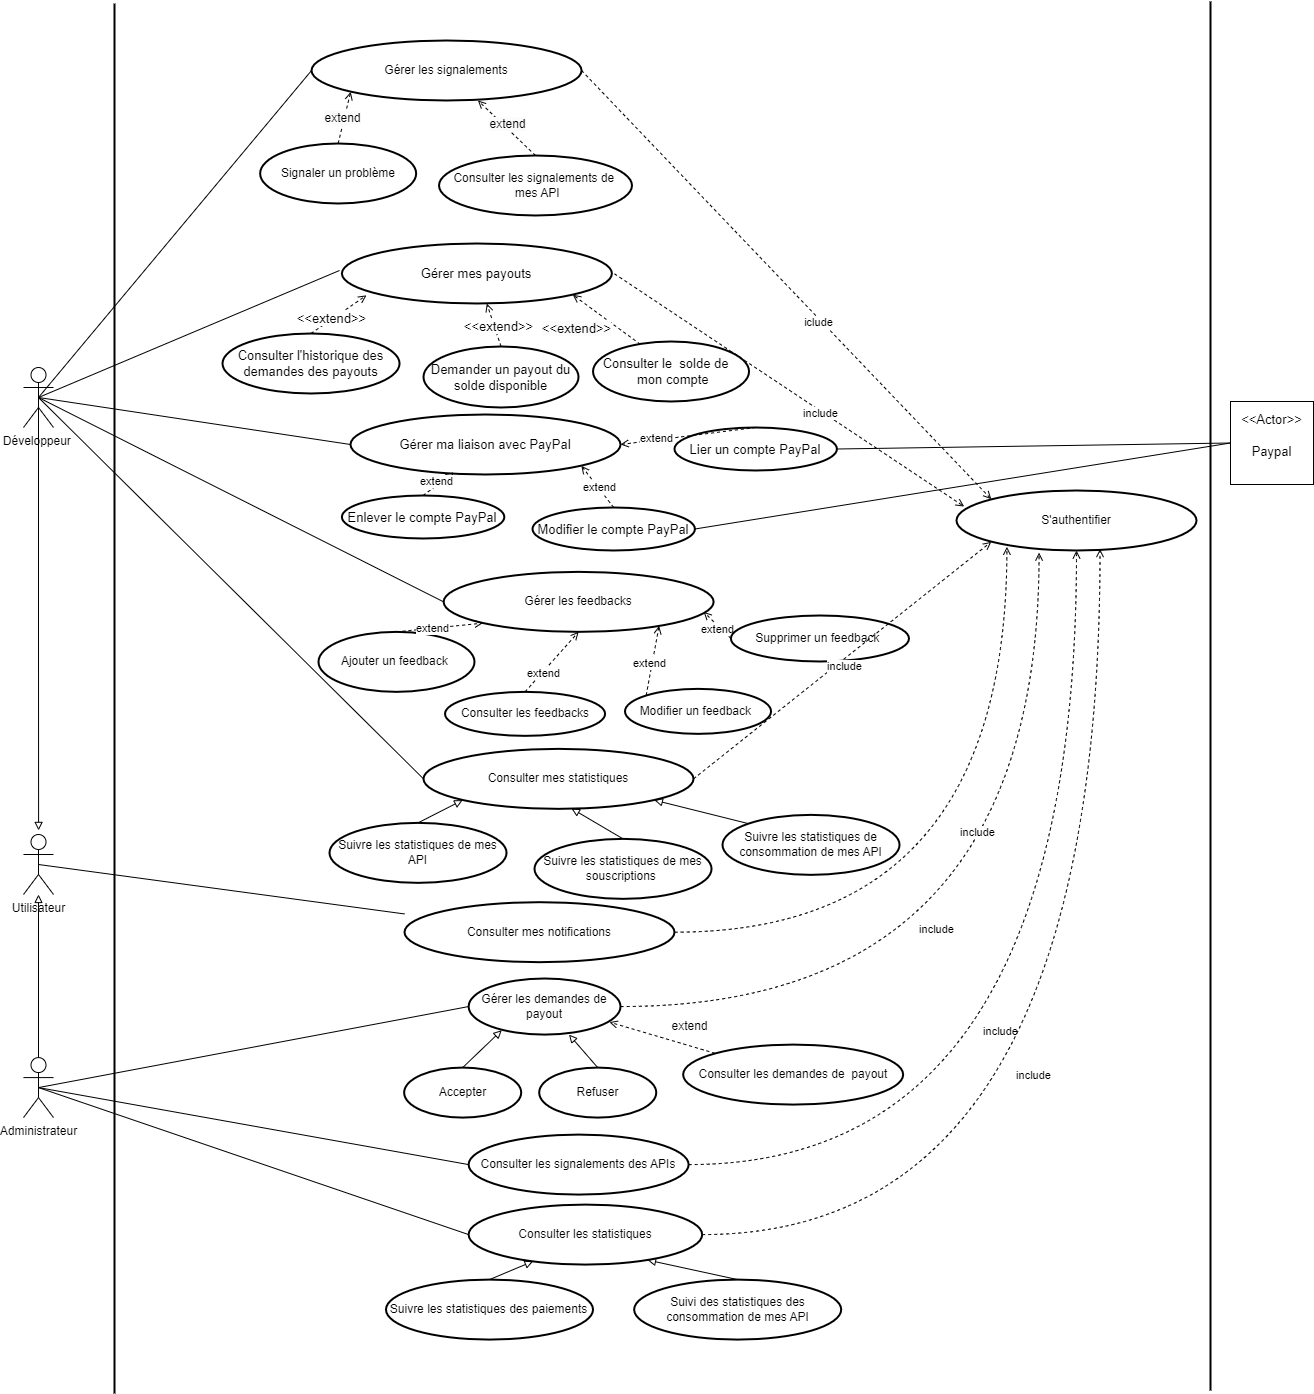
\includegraphics[width=1.1\columnwidth]{diagrammedecasdutilisationensprint3.png}}
    \caption{Diagramme de cas d'utilisation du sprint 3 }
    \label{fig:logo_tt}
\end{figure}

\pagebreak
\subsection{Exemple d'une maquette d'interface du sprint 3}

La figure suivante représente la maquette du tableau de bord de statistique des payouts réalisés dans la marketplace.
\begin{figure}[H]
    \centering
    \frame{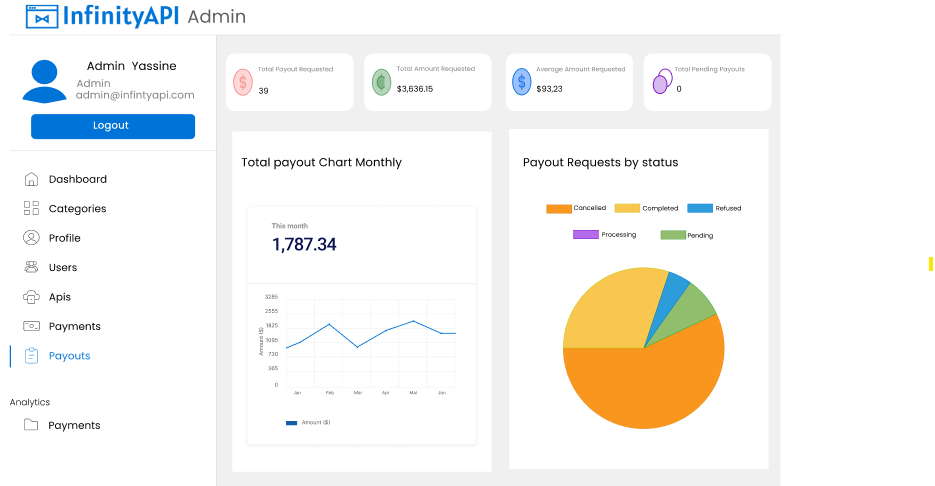
\includegraphics[width=1.1\columnwidth]{interfacedestatistiquedespayout.png   }}
    \caption{Maquette de statistiques des payouts réalisés sur la plateforme   }
    \label{fig:logo_tt}
\end{figure}
\pagebreak

\section{ Conception}
Dans cette partie, nous allons présenter la modélisation structurelle à travers le diagramme de classes et le diagramme de déploiement avant de présenter les principaux traitements de sprint relatifs à :
\begin{itemize}	
   \item La demande de payout
   \item L'ajout d'un rapport 
   \item L'ajout  de statistiques détaillé en annexe 1 
\end{itemize}
\subsection{Modélisation structurelle}
\subsubsection{Diagramme du classes}

\textbf{a. Règles de gestion et calcul} \\
Voici les principales règles de gestion avant de présenter le diagramme de classes :

    \begin{itemize}
        \item  Un développeur peut soumettre zéro ou plusieurs feedbacks.
        \item Chaque feedback est soumis par un seul développeur.
        \item Un feedback est relatif à une API.
        \item Une API peut avoir zéro ou plusieurs feedbacks.
        \item Un développeur peut avoir zéro ou plusieurs notifications.
        \item Chaque notification est associée à  un seul développeur.
        \item Un développeur peut signaler zéro ou plusieurs rapports.
        \item Chaque rapport est signalé par un seul développeur.
        \item Un développeur peut réaliser zéro ou plusieurs payouts.
        \item Chaque payout est réalisé par un seul développeur.

    \end{itemize}
\pagebreak

\textbf{b. Diagramme de classes } \\

\begin{figure}[H]
    \centering
    \frame{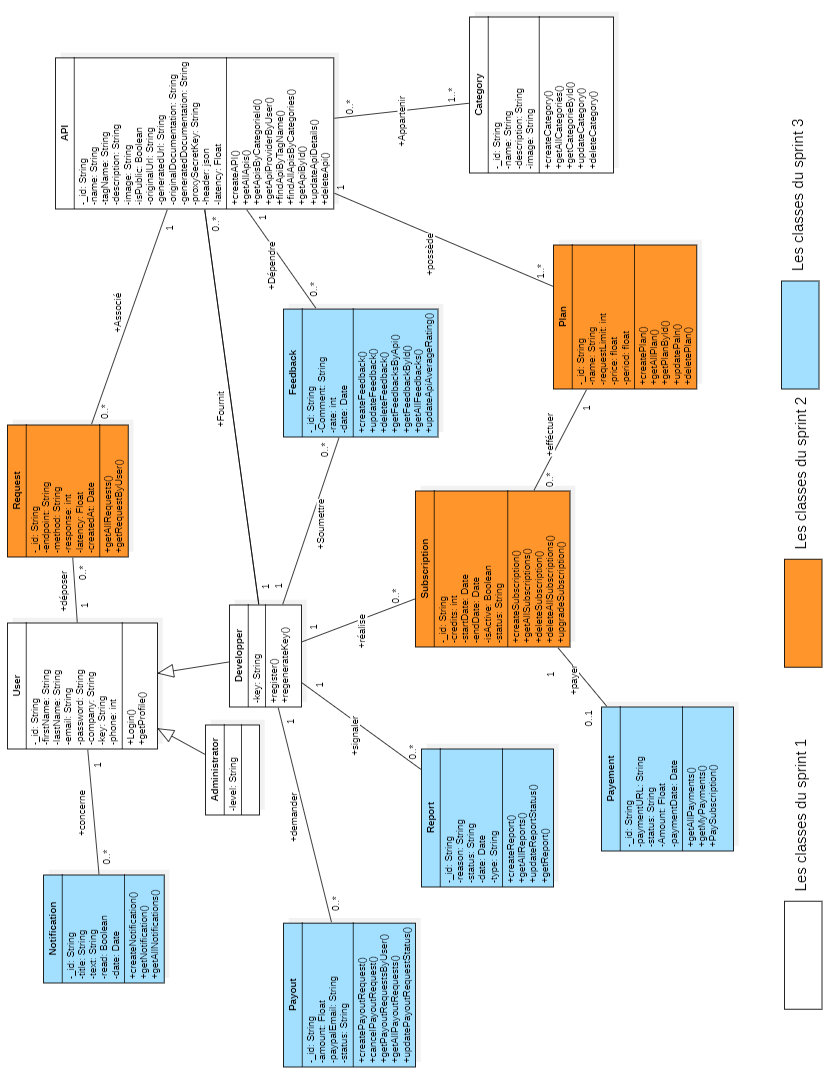
\includegraphics[width=1\columnwidth]{Diagrammedeclassedesprint3.png    }}
    \caption{Diagramme de classes du sprint 3    }
    \label{fig:logo_tt}
\end{figure}
La représentation NoSql associée à notre base de données est présentée en annexe 1

\subsubsection{Diagramme de déploiement}

Le diagramme de déploiement illustre l'architecture de l'application "InfinityAPI", montrant les interactions entre ses différents composants. Le client utilise un navigateur web pour accéder à l'application via HTTP/HTTPS. Le serveur web héberge l'interface utilisateur (InfinityAPI Frontend) et communique avec le servec backend de l'application (InfinityAPI Backend) fonctionnant dans un environnement Node.js. Le backend communique avec les fournisseurs de services API externes et les passerelles de paiement, Stripe et PayPal, également via HTTP/HTTPS, pour gérer les transactions financières. Pour le stockage et la récupération des données, le backend utilise une base de données MongoDB hébergée sur MongoDB Atlas, accessible via TCP/IP. Cette architecture assure une interaction fluide entre le client, les services externes, et la base de données, tout en maintenant la sécurité et l'efficacité des transactions et des traitements de données.
\begin{figure}[H]
    \centering
    \frame{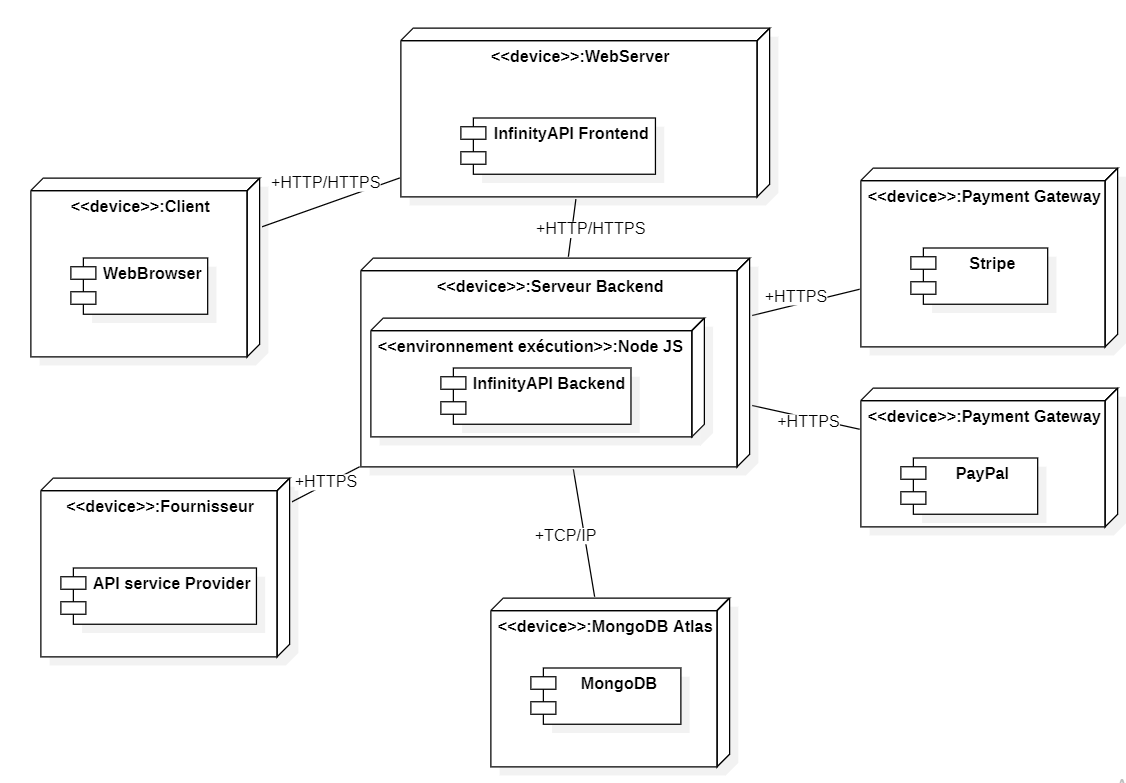
\includegraphics[width=1\columnwidth]{diagrammededeploiement.png}}
    \caption{Diagramme de déploiement}
    \label{fig:logo_tt}
\end{figure}
\pagebreak

\subsection{Diagramme d'état "Demande d'un payout"}
Le processus de demande de payout passe par plusieurs états :
\begin{itemize}
    \item \textbf{Pending (En attente) :} Cet état est atteint lorsque le développeur crée une demande de payout. La demande est en attente d'acceptation ou de rejet par l'administrateur.
    \item \textbf{Processing (En cours de traitement) :} Cet état indique que la demande de payout a été acceptée et est actuellement en cours de traitement par l'administrateur.
    \item \textbf{Completed (Terminée) :} Cet état indique que la demande de payout a été complétée avec succès. L'administrateur a finalisé le traitement de la demande.
    \item \textbf{Refused (Refusée) :} Cet état indique que la demande de payout a été rejetée par l'administrateur.
    \item \textbf{Cancelled (Annulée) :} Cet état indique que la demande de payout a été annulée par le développeur avant ou durant le traitement.
\end{itemize}
La figure suivante illustre le diagramme d’état relatif à une demande de payout.
\begin{figure}[H]
    \centering
    \frame{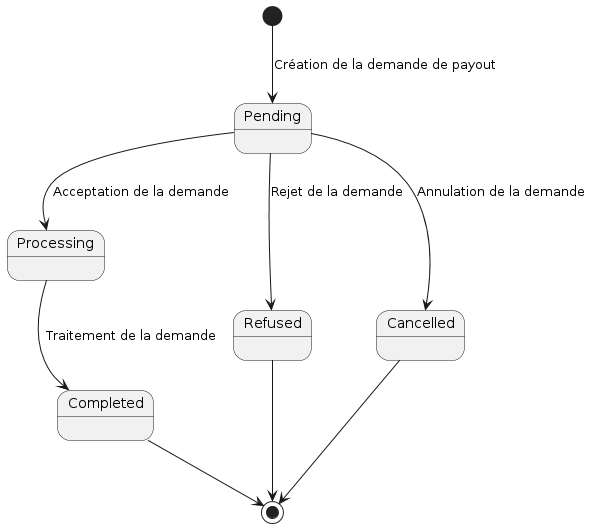
\includegraphics[width=0.9\columnwidth]{digrammedetatsouscription.png}}
    \caption{Diagramme d'état "Demande d'un payout"}
    \label{fig:logo_tt}
\end{figure}

\pagebreak

\subsection{Diagramme de séquence "Demande de payout"}
Ce diagramme de séquence illustre les interactions entre les différents composants de la marketplace lors d'une demande de solde(payout request). Tout d'abord, le développeur soumet un payout request. Une requête HTTP est alors envoyée au backend, qui vérifie la validité du jeton d'authentification. Si le jeton est invalide, un message d'erreur "invalid token" est renvoyé. Si le jeton est valide, le backend vérifie si le compte du développeur est lié à un compte PayPal. Si ce n'est pas le cas, un message d'erreur "You have no linked PayPal account" est affiché. Si le compte PayPal est lié, le backend vérifie si le solde du compte est supérieur à 0et si la dernière demande de paiement date de plus de 30 jours. Si toutes ces conditions sont remplies, la demande de paiement est acceptée, le solde du compte est mis à jour à zéro, et un message de succès est affiché pour indiquer que la demande de paiement a été ajoutée avec succès.

\begin{figure}[H]
    \centering
    \frame{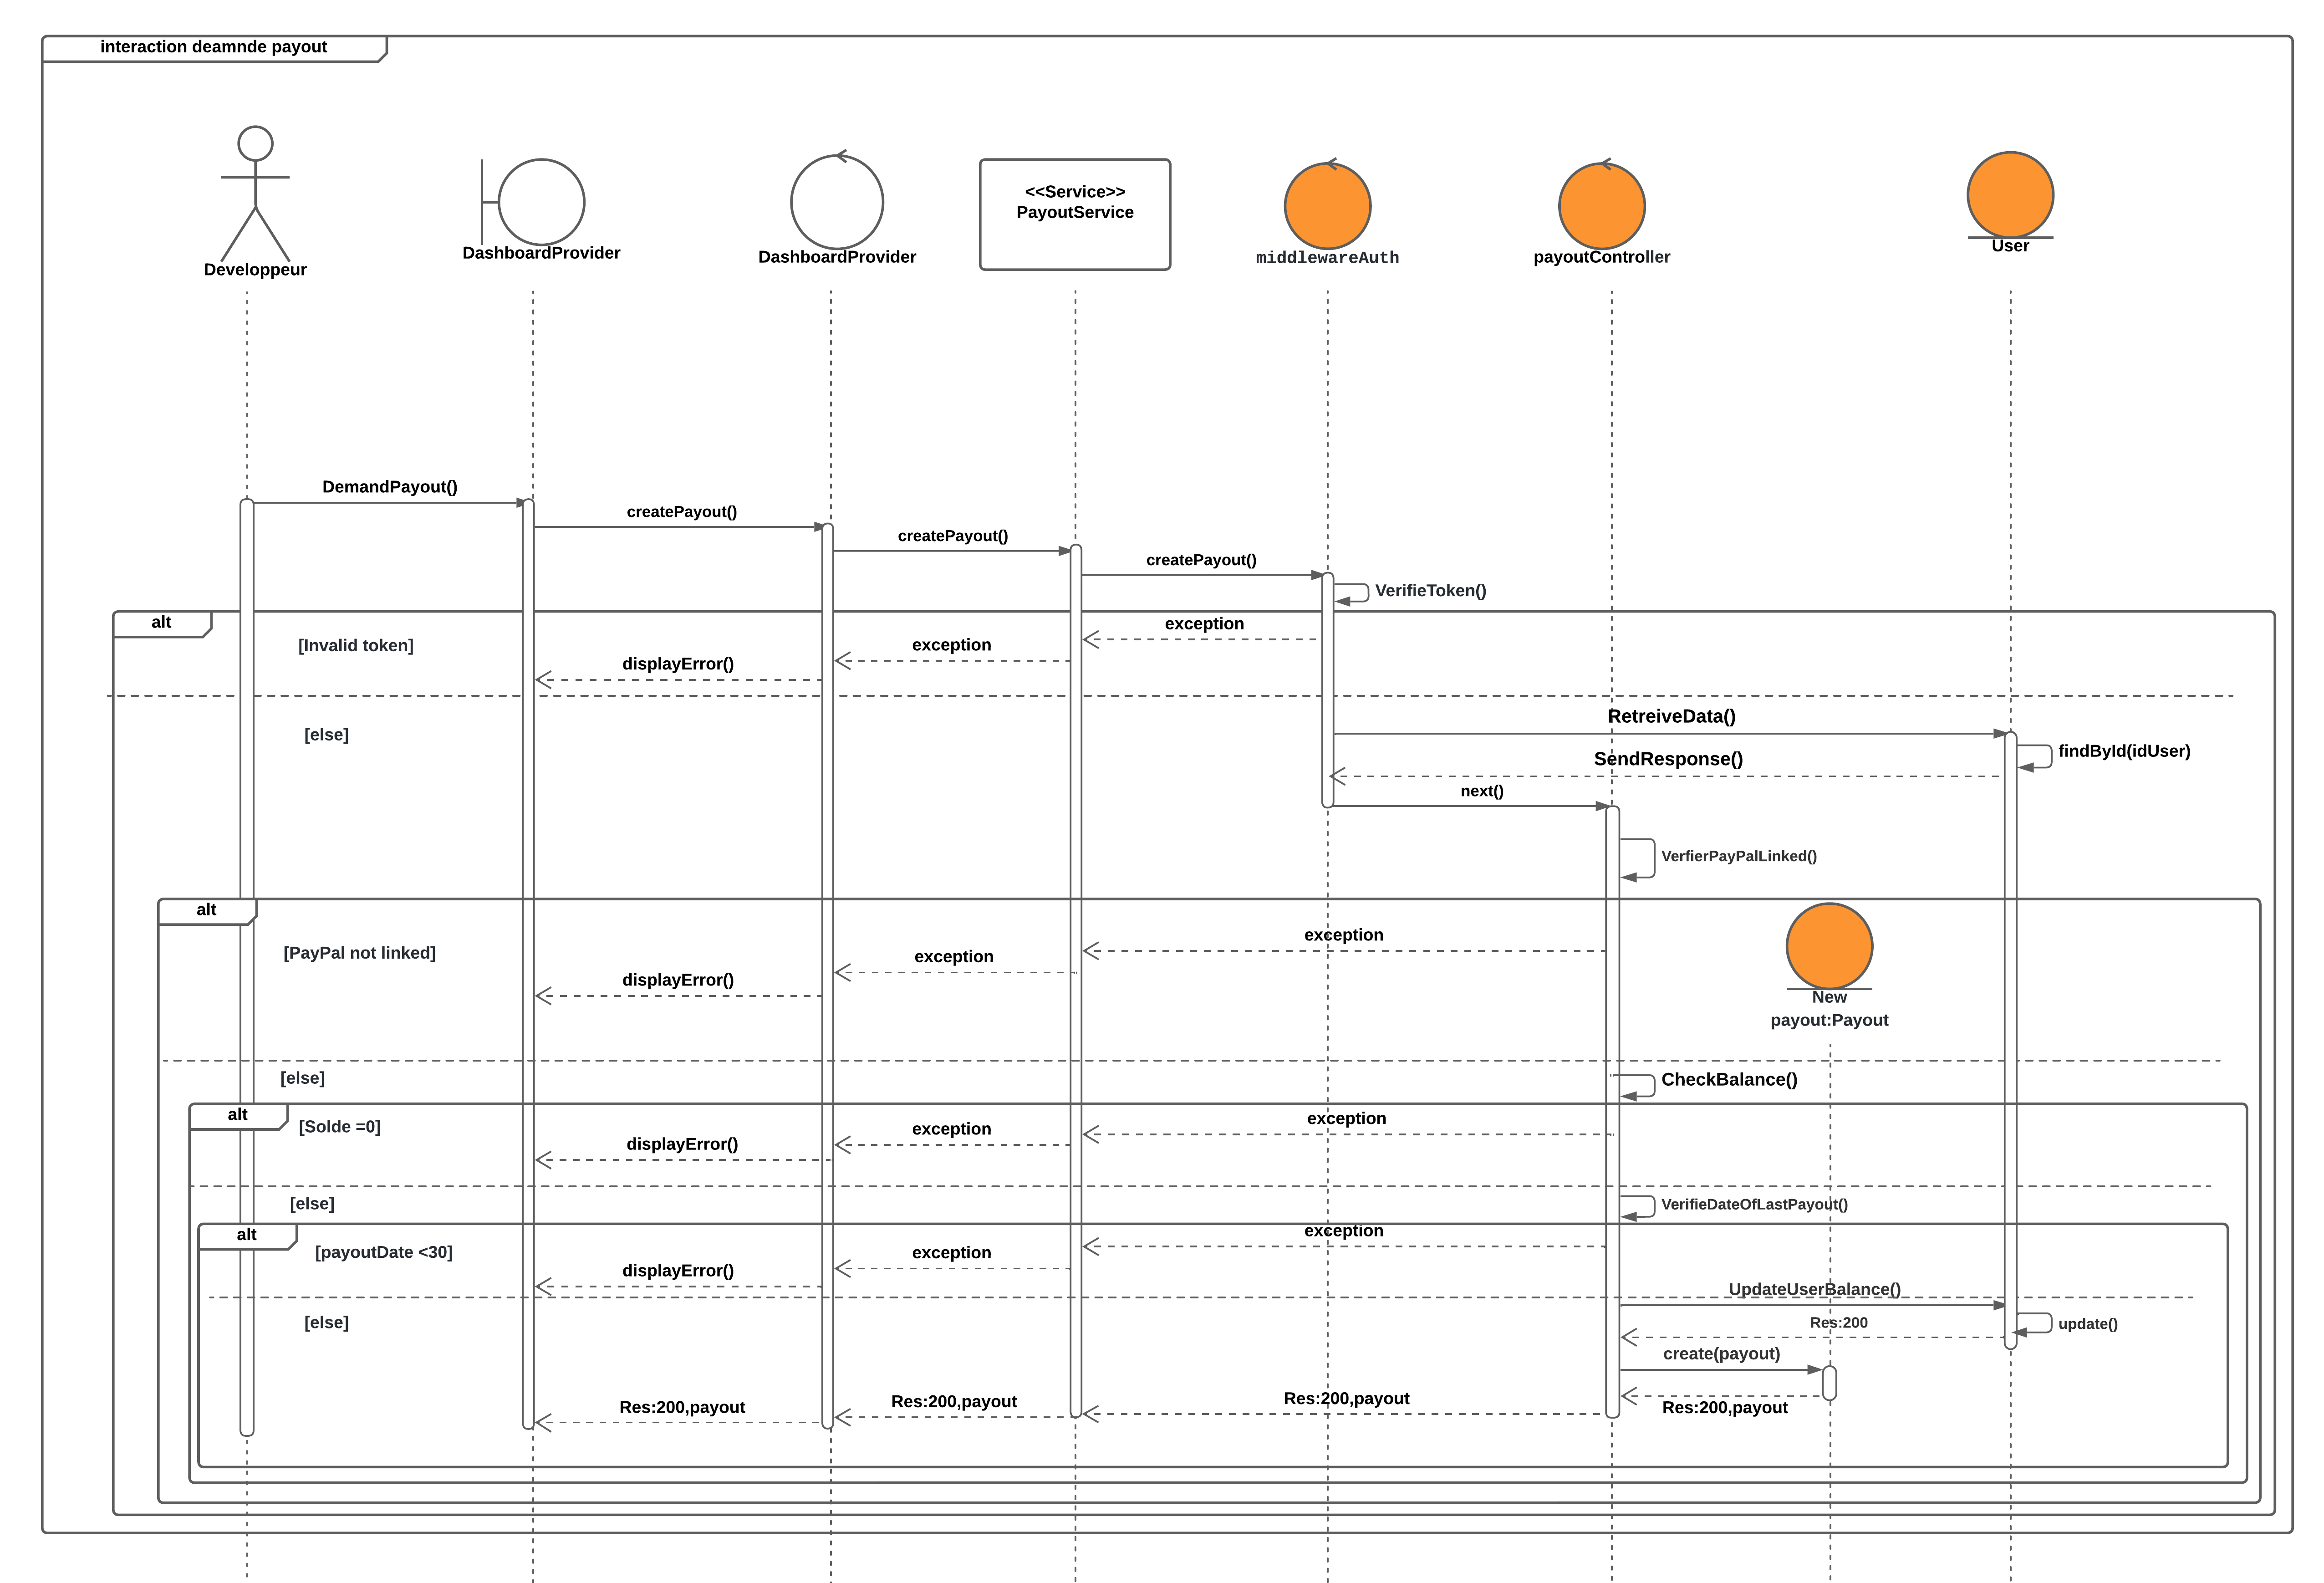
\includegraphics[width=1.1\columnwidth]{diagrammedesequencepayoutrequest.png }}
    \caption{Diagramme de séquence "Demande de payout" }
    \label{fig:logo_tt}
\end{figure}
\pagebreak



\subsection{Diagramme de séquence "Ajouter rapport"}
Ce diagramme de séquence illustre l'enchaînement des interactions entre les différents composants de la marketplace pour l'ajout d'un rapport signalant une erreur. Le développeur remplit le formulaire d'ajout d’un signalement. Si les champs sont invalides, un message d'erreur est affiché. Sinon, une requête HTTP est envoyée au backend. Le backend vérifie alors la validité du jeton. Si le jeton est invalide, un message d'erreur "invalid token" est renvoyé. Sinon, un message de succès est affiché pour indiquer que le rapport a été ajouté avec succès.

\begin{figure}[H]
    \centering
    \frame{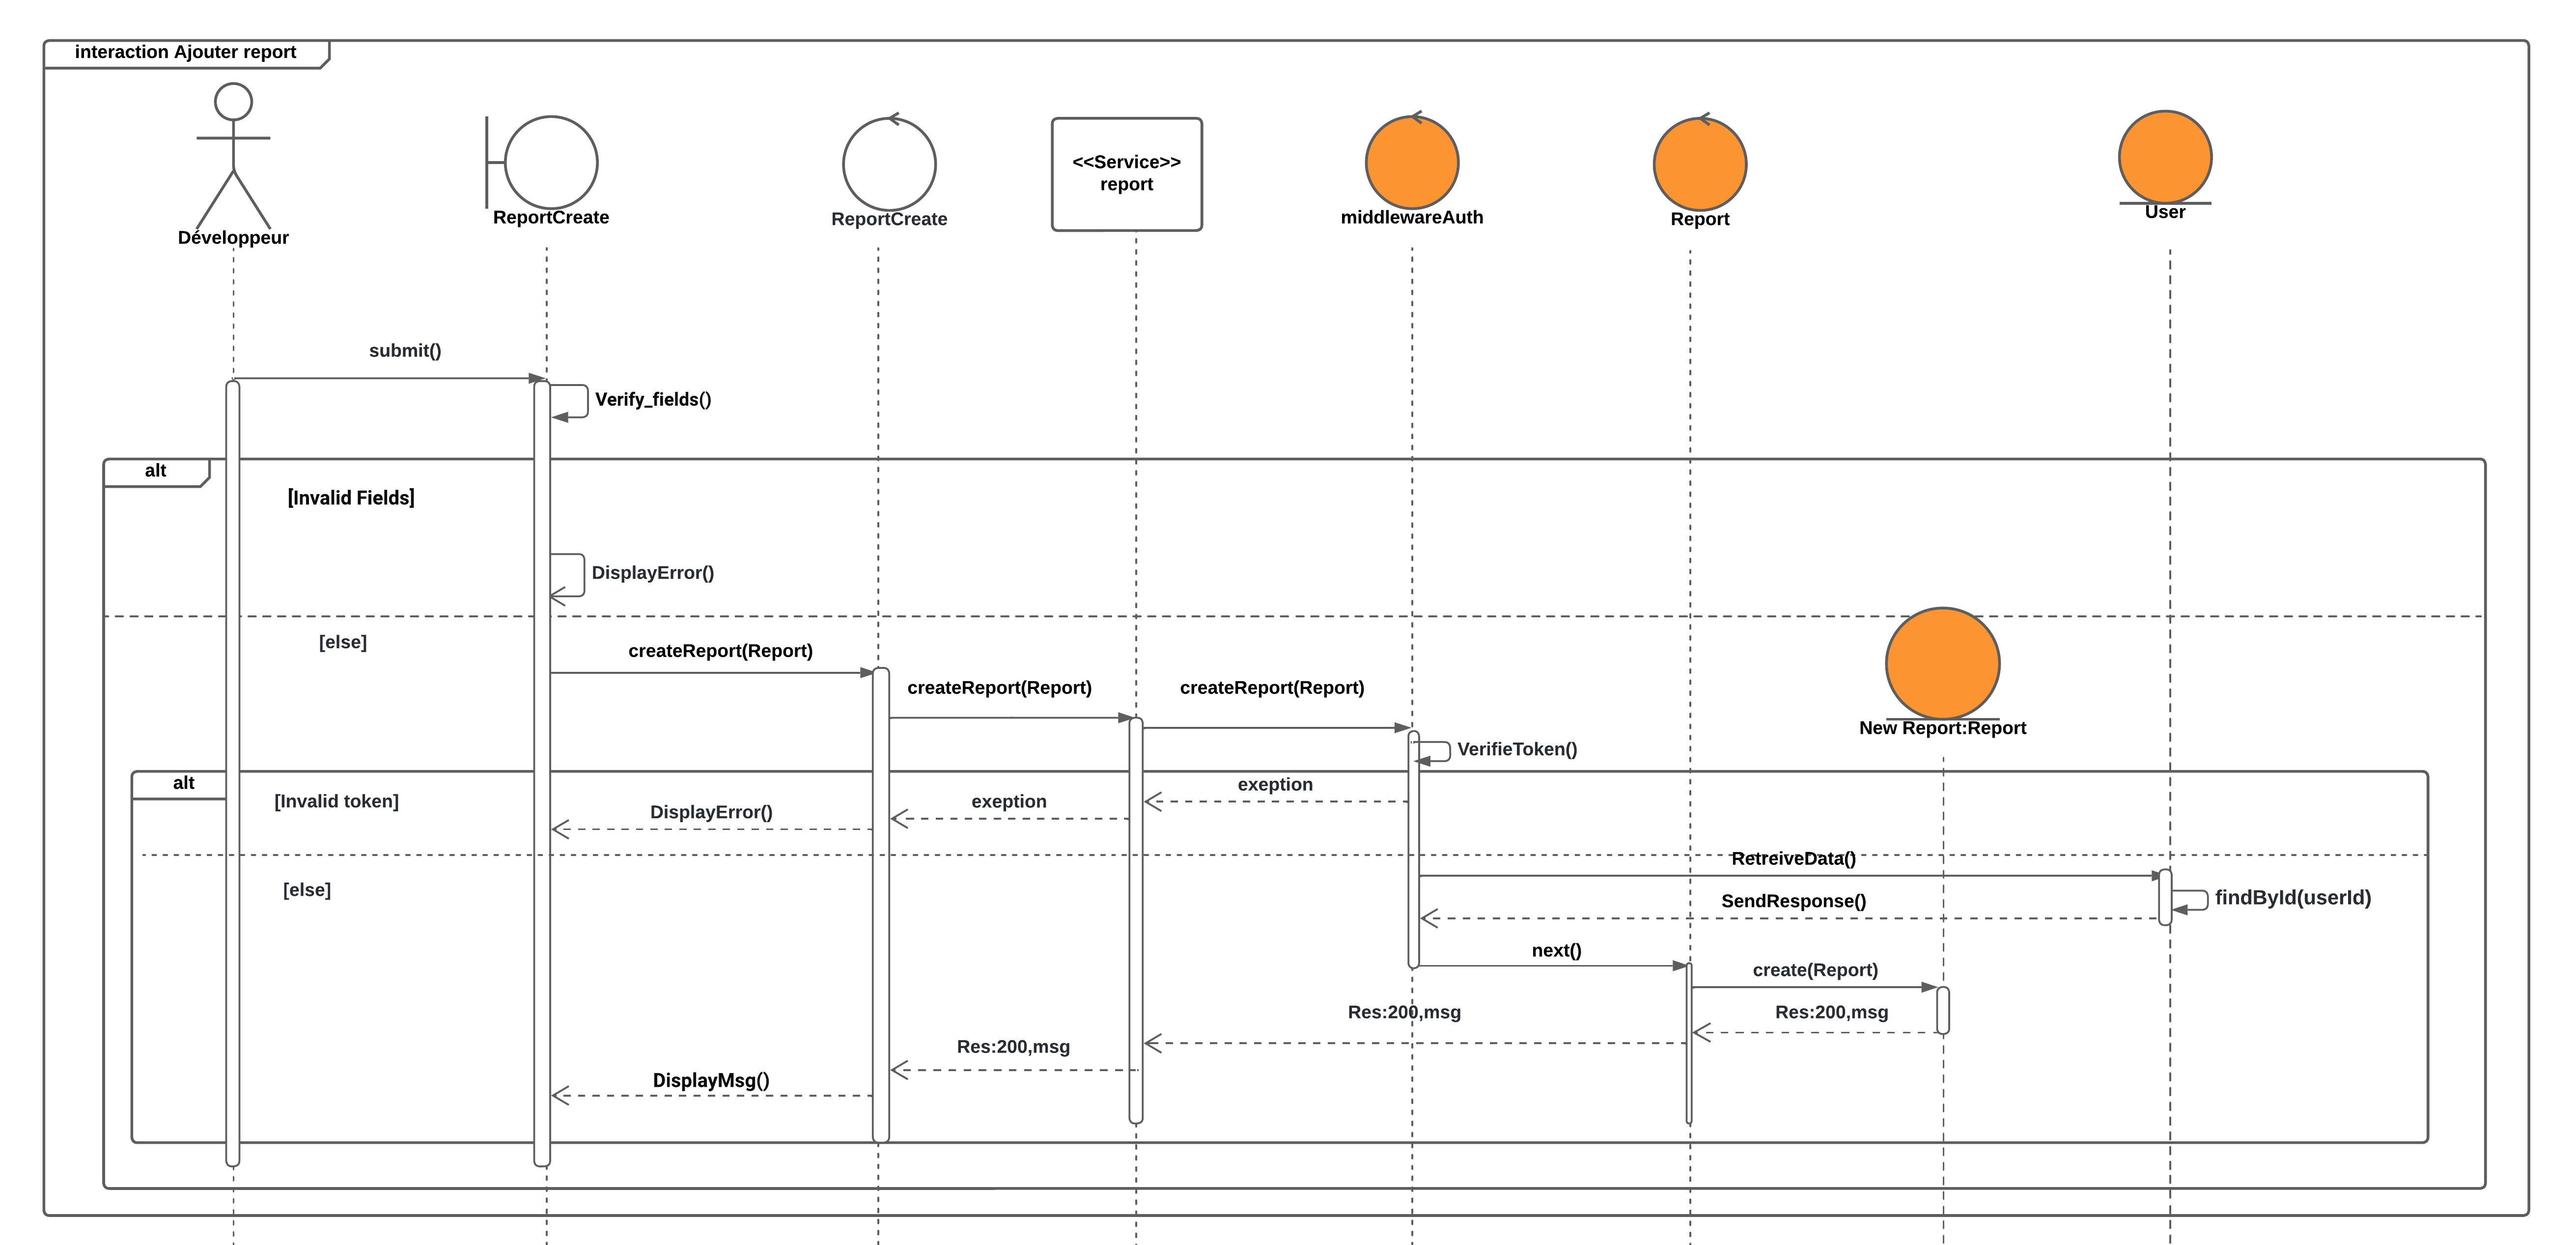
\includegraphics[width=1.1\columnwidth]{diagrammedesequenceAjouterReport.png  }}
    \caption{Diagramme de séquence "Ajouter rapport"    }
    \label{fig:logo_tt}
\end{figure}






\section{ Revue de sprint }
Dans cette partie, nous allons exposer le travail réalisé durant le sprint 3, ainsi que le
burndown chart et la rétrospective.
    \subsection{Réalisation}
    Dans cette étape, nous allons explorer les principales interfaces réalisées lors de ce sprint.
    \pagebreak
    \subsubsection{Gestion des demandes de payout}
    Cette interface représente le processus de demande d'un payout.
    \begin{figure}[H]
        \centering
        \frame{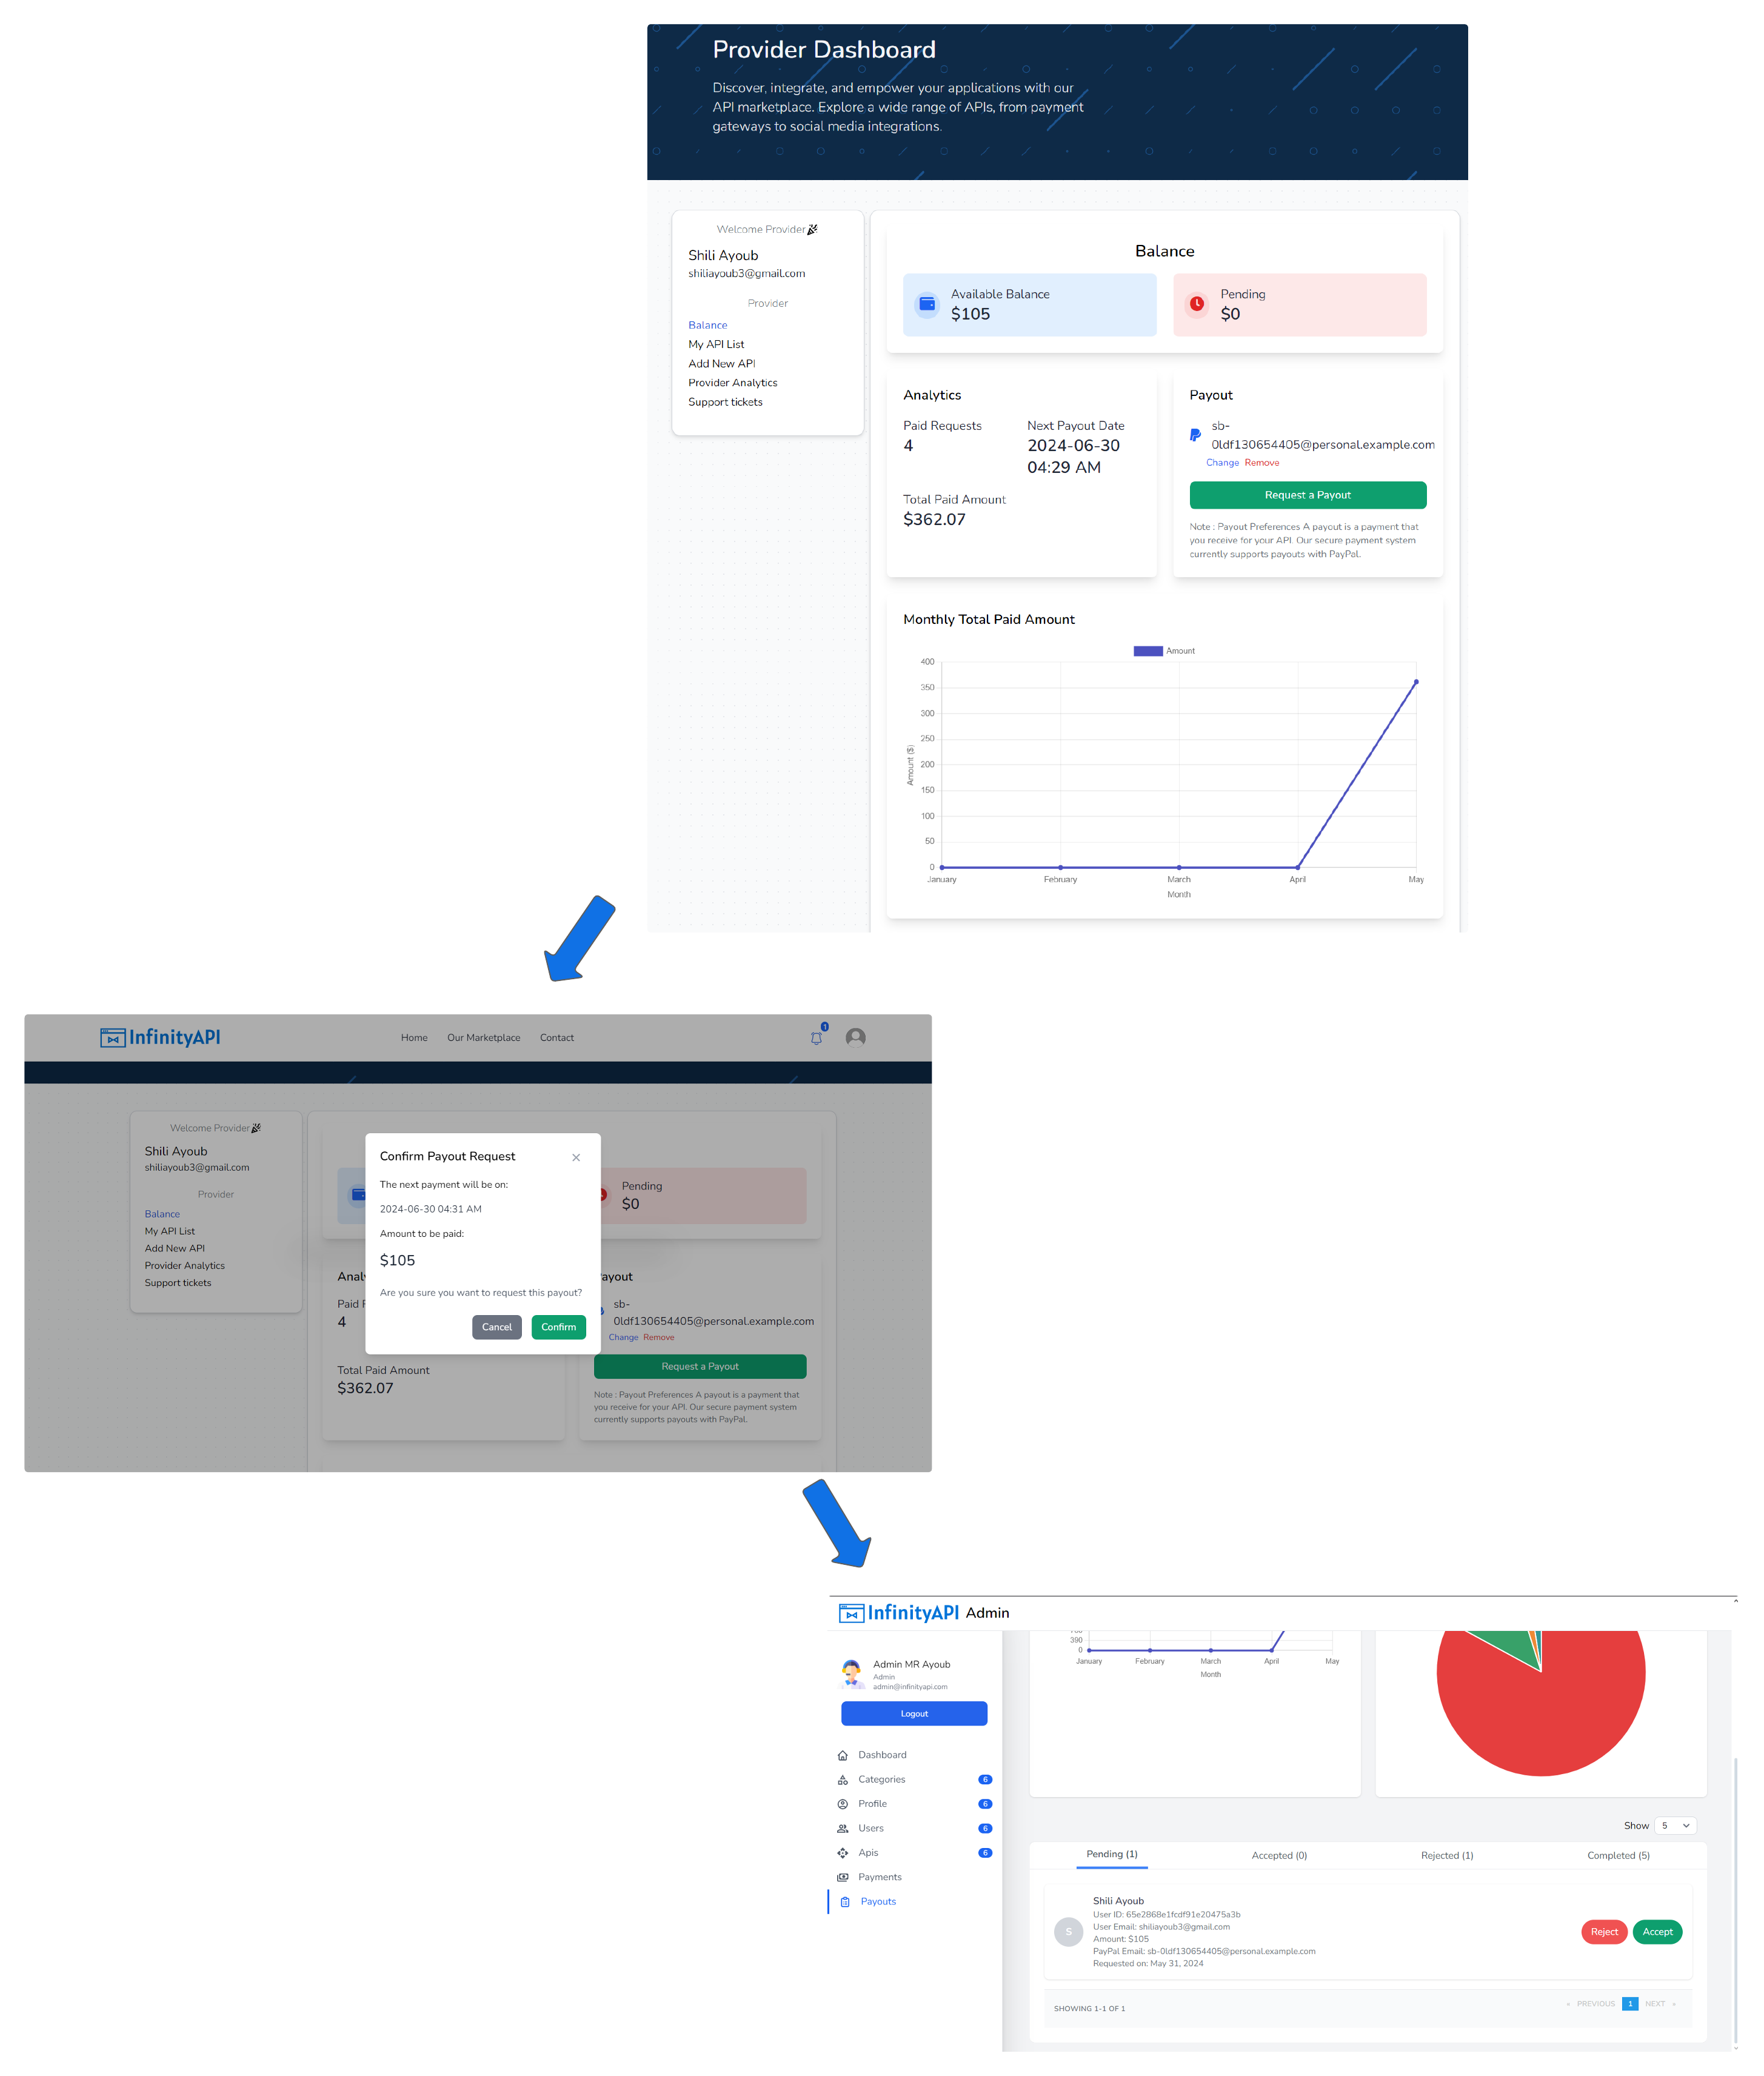
\includegraphics[width=1.1\columnwidth]{processusdepayout.png}}
        \caption{Interface du processus de payout  }
        \label{fig:logo_tt}
    \end{figure}

    \subsubsection{Dashboard de statistiques}
    Cette interface ,destinée au fournisseur d'API, affiche les statistiques des souscriptions, des requêtes et de la latence de ses API. 
    \begin{figure}[H]
        \centering
        \frame{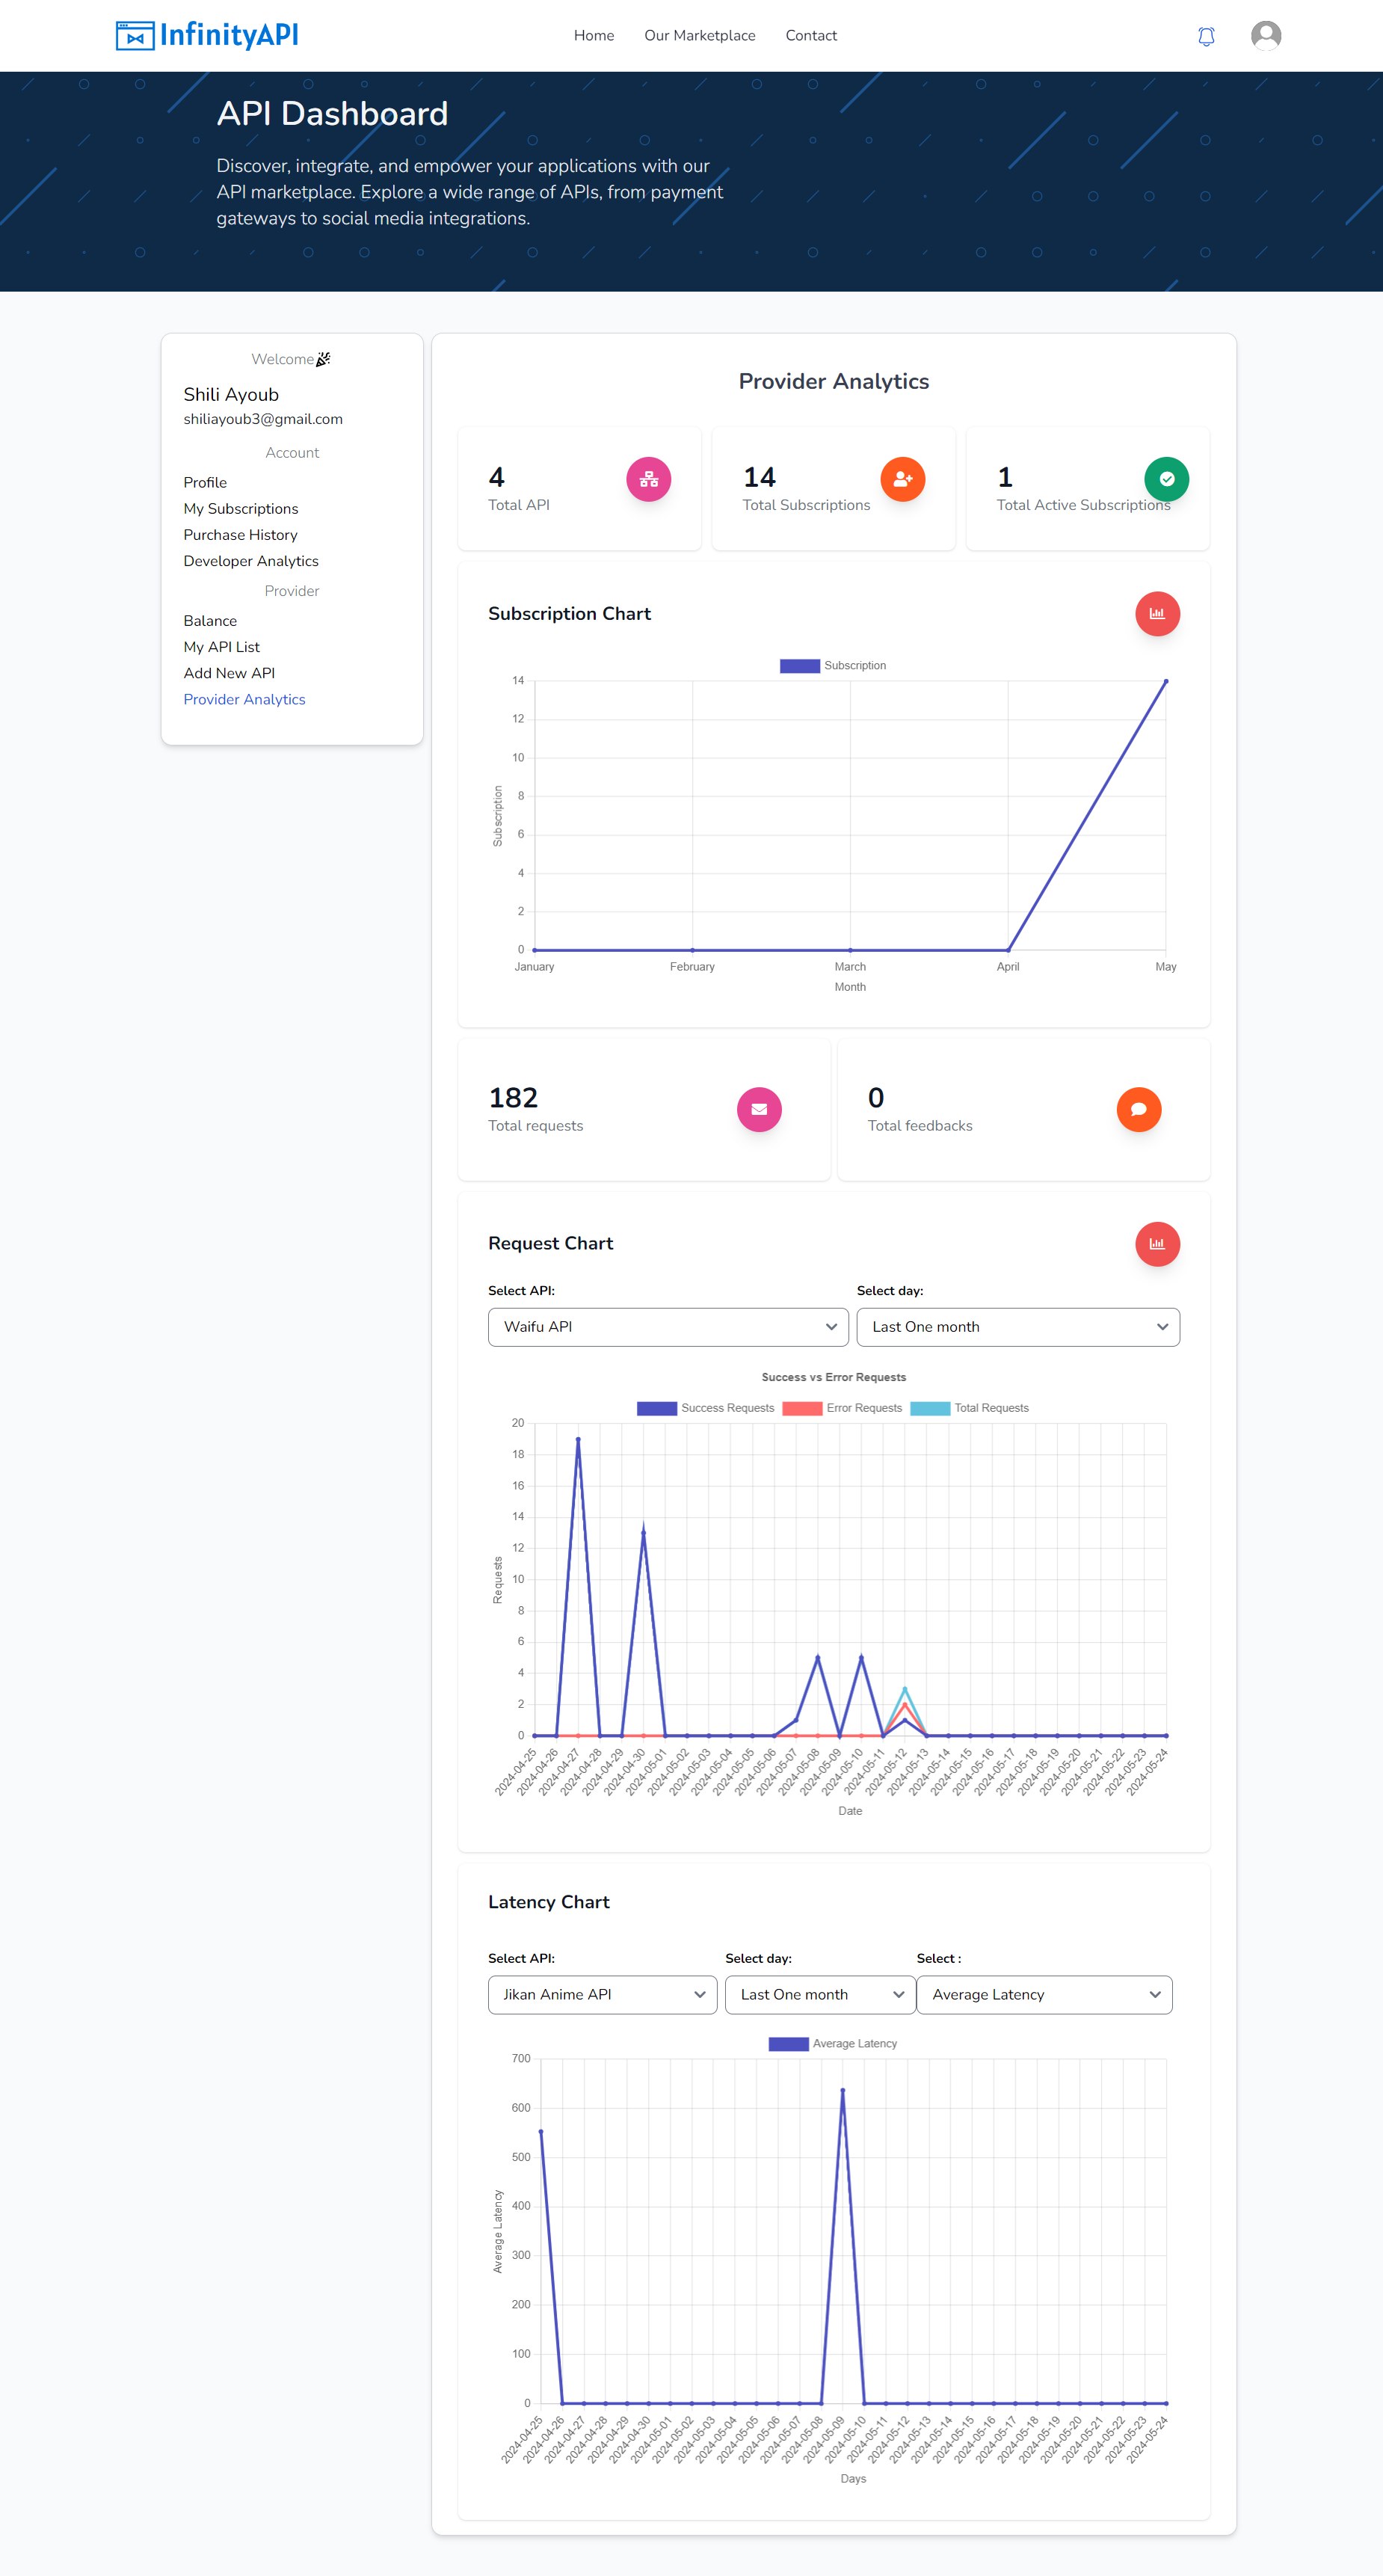
\includegraphics[width=0.7\columnwidth]{ InterfaceduproviderdeAPI.png}}
        \caption{ Interface du fournisseur d'API }
        \label{fig:logo_tt}
    \end{figure}


    Cette interface affiche deux statistiques de paiement effectuées dans la marketplace par mois et par catégorie.
    \begin{figure}[H]
        \centering
        \frame{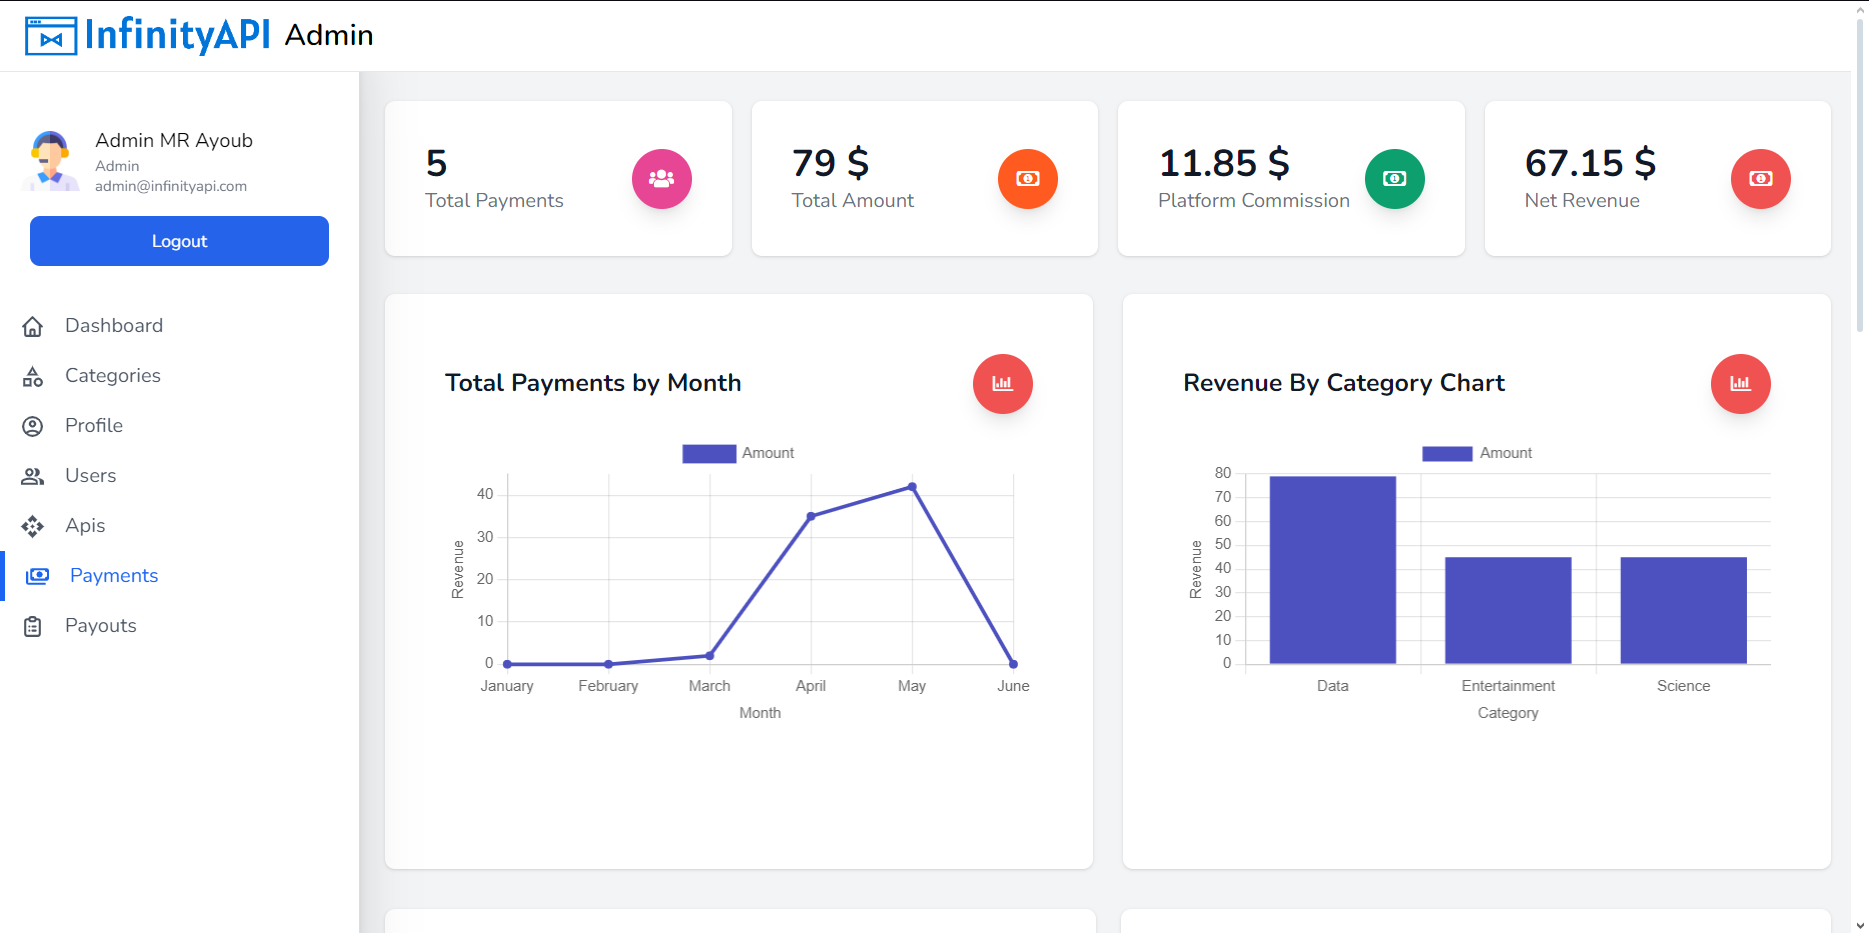
\includegraphics[width=1\columnwidth]{interfacedestatistiquedespayement.png }}
        \caption{ Interface du statistique de paiement }
        \label{fig:logo_tt}
    \end{figure}

    \subsubsection{Gestion des feedbacks}

    Cette interface représente le processus de l'ajout d'un feedback 
    \begin{figure}[H]
        \centering
        \frame{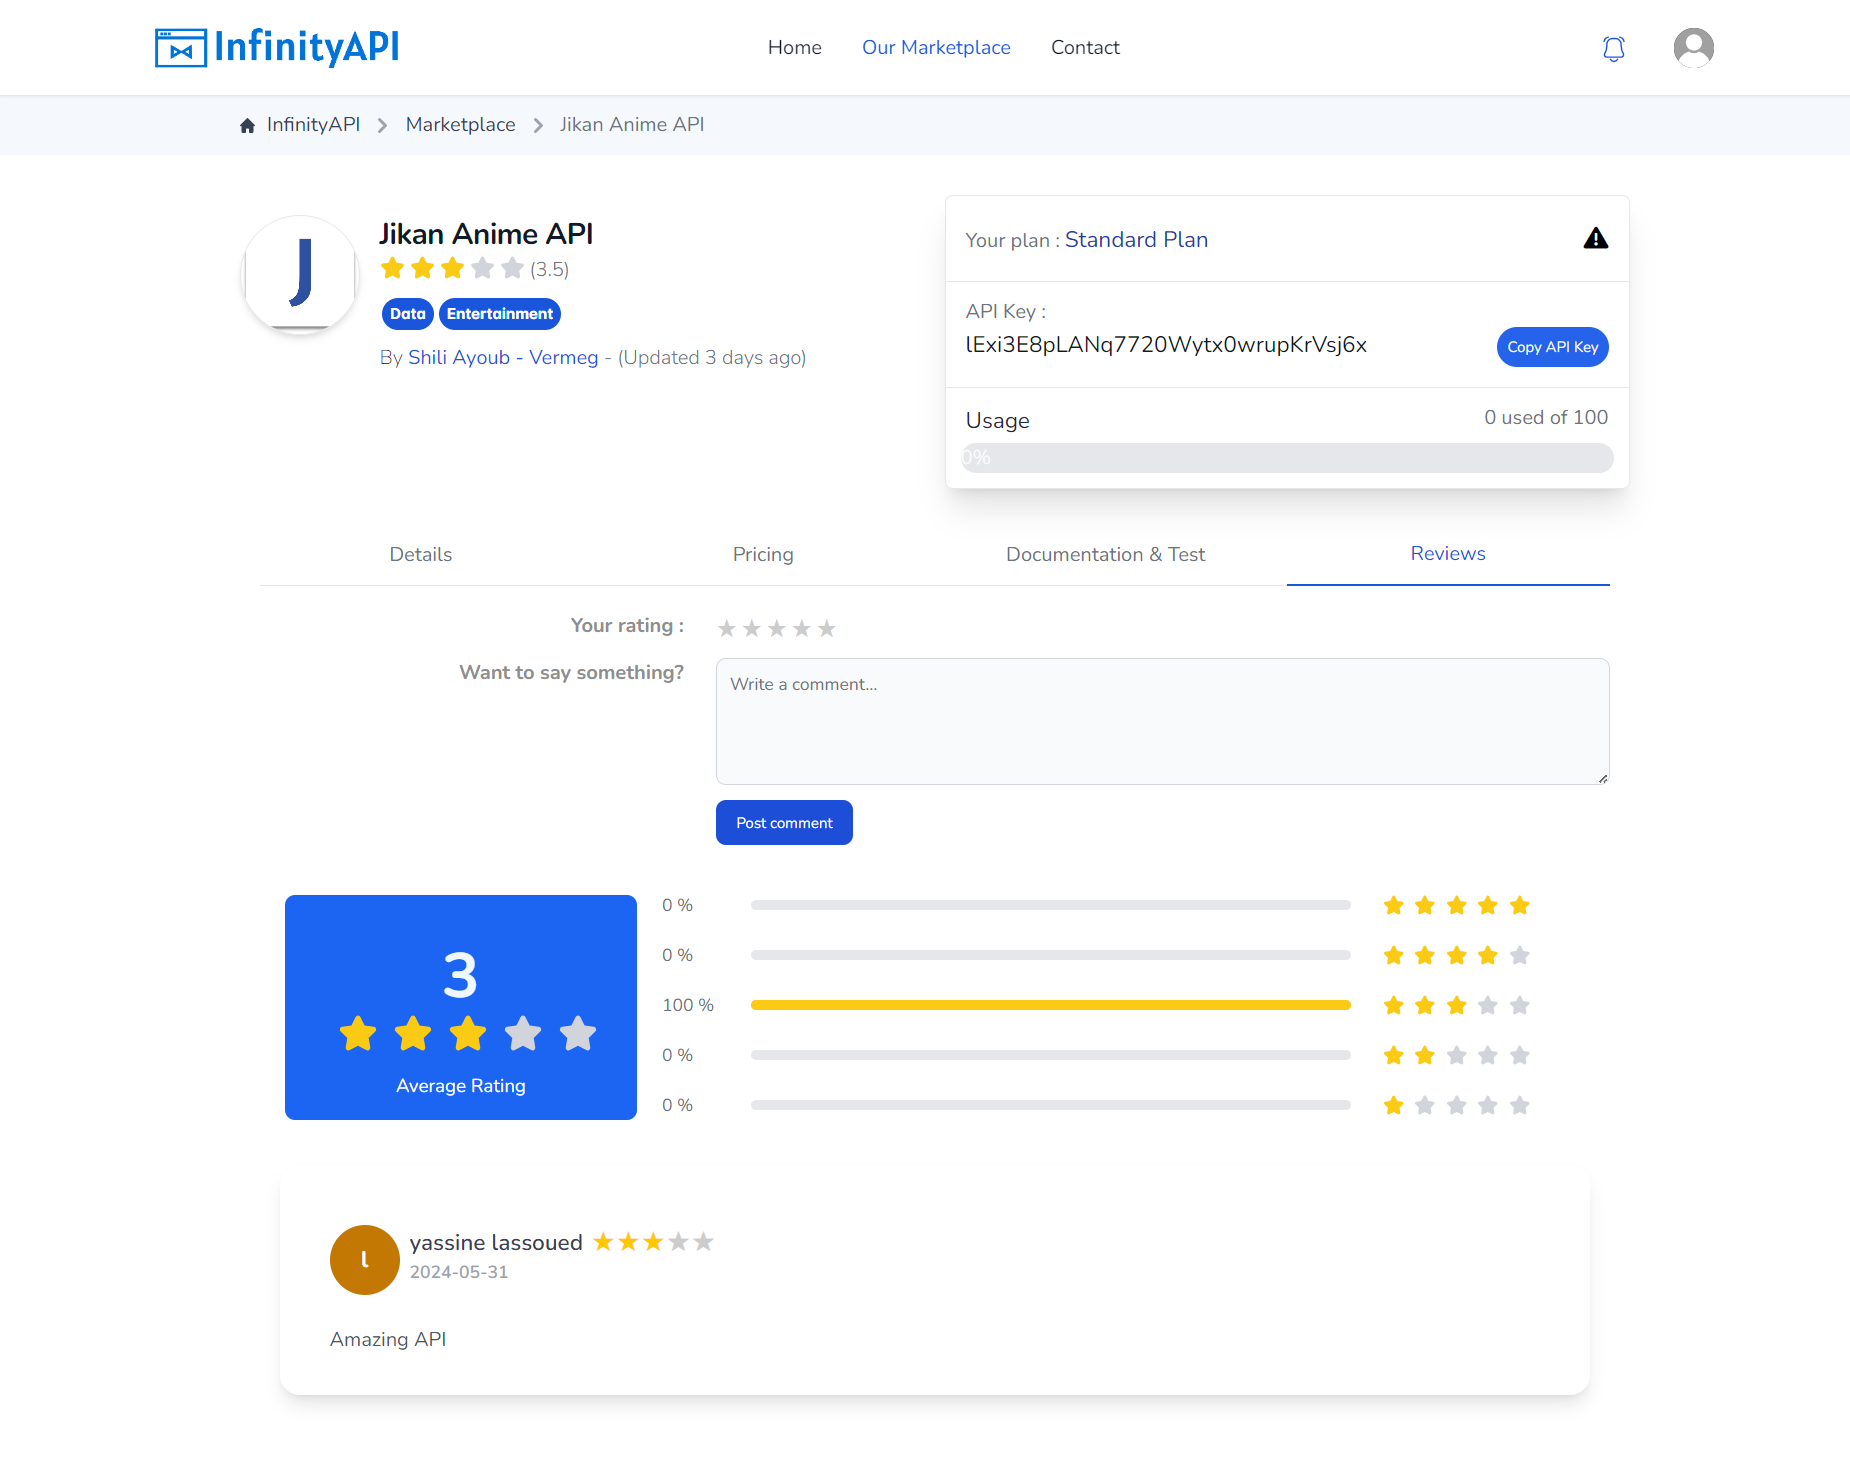
\includegraphics[width=0.8\columnwidth]{   interfacedeprocessusdegestiondunfeedback.png}}
        \caption{ Interface du feedback }
        \label{fig:logo_tt}
    \end{figure}
    \subsubsection{Liste des notifications}

    Cette interface représente la liste des notifications reçu par le développeur en temps réel. 
    \begin{figure}[H]
        \centering
        \frame{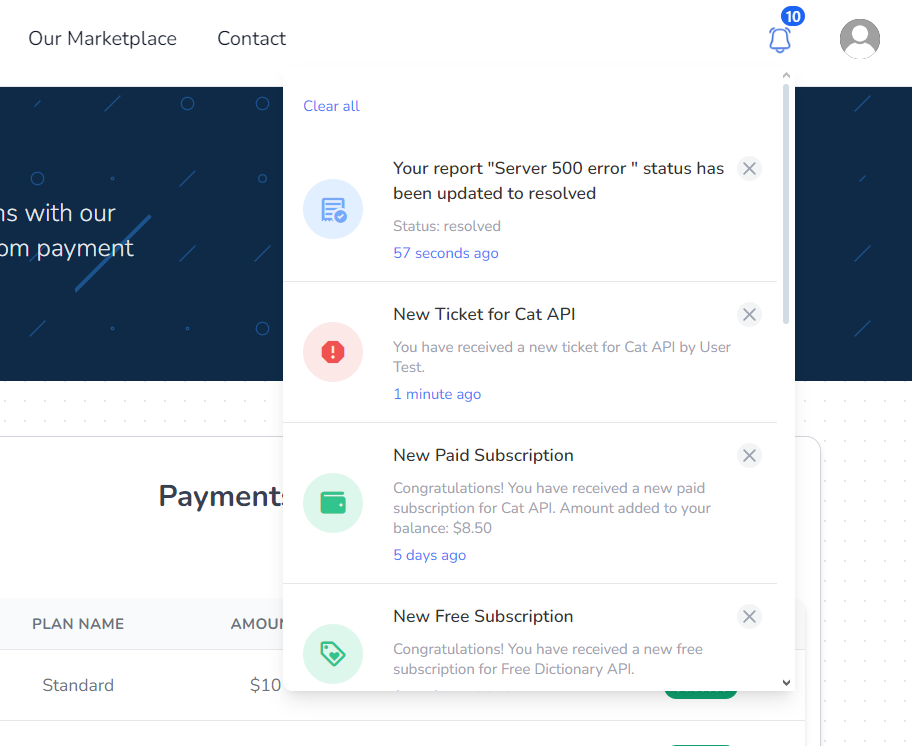
\includegraphics[width=0.8\columnwidth]{  interfacenotification.png }}
        \caption{ Interface de la liste des notifications}
        \label{fig:logo_tt}
    \end{figure}
    
\pagebreak
    \subsection{Burndown Chart}
    \begin{figure}[H]
        \centering
        \frame{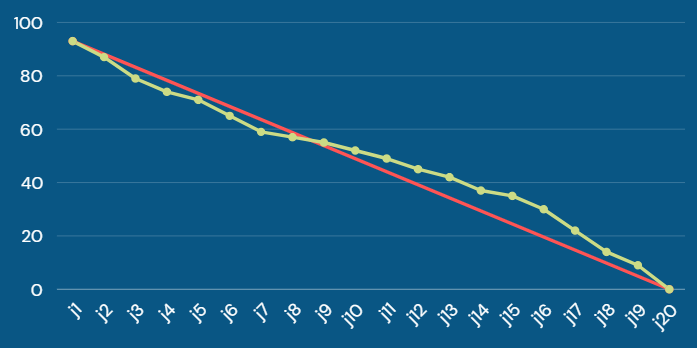
\includegraphics[width=1\columnwidth]{burndownchartsprint3.png}}
        \caption{Burndown chart du sprint 3 }
        \label{fig:logo_tt}
    \end{figure}
    Ce burndown montre que :
    \begin{itemize}
        \item Tous les user stories sont réalisés dans le temps estimé.
        \item La vélocité de notre équipe est 93.
    \end{itemize}
    

    \subsection{Rétrospective du sprint 3}
    \begin{longtable}[c]{|p{0.3\linewidth}|p{0.6\linewidth}|}
        \hline
        \textbf{Les questions} & \textbf{Les réponses} \\
        \hline
        \endfirsthead
        \multicolumn{2}{c}%
        {{\bfseries \tablename\ \thetable{} -- suite de la page précédente}} \\
        \hline
        \textbf{Les questions} & \textbf{Les réponses} \\
        \hline
        \endhead
        \hline \multicolumn{2}{|r|}{{\bfseries Suite à la page suivante}} \\
        \hline
        \endfoot
        \hline
        \endlastfoot
    
        \multirow{2}{=}{Ce qui s'est bien passé} & Achèvement des travaux dans le temps estimé \\
        &Le projet a été validé par le Product Owner\\
        \hline
        \multirow{2}{=}{Les problèmes rencontrés} & Manque de repos \\
        &Difficultés lors de la fusion du code 
      
    \end{longtable}

\section*{Conclusion}
Au cours de ce dernier chapitre, nous avons présenté la spécification fonctionnelle, la conception, ainsi que la revue et la rétrospective de ce dernier sprint. Ce chapitre marque la fin du cycle de développement Scrum, aboutissant à un travail exécutable.

        \clearpage

        \chapter*{Conclusion générale}
\addcontentsline{toc}{chapter}{Conclusion générale}
\markboth{Conclusion générale}{}


En guise de conclusion, notre projet de fin d’études réalisé au sein de Vermeg porte sur la conception et le développement d'une marketplace d’API nommée "InfinityAPI". Ce projet a pour objectif d'offrir une plateforme où les développeurs peuvent aussi bien proposer et monétiser leurs propres API que souscrire et consommer une large gamme d'API proposées.  \\
Pour la réalisation technique, nous avons adopté l’architecture MEAN pour le développement de la marketplace. Ce projet a été une véritable expérience enrichissante, nous permettant d’acquérir de nombreuses compétences.\\ Nous avons ainsi mieux maîtrisé les framewoks utilisés et découvert des biblithèques et des outils de développement, tels que Swagger pour la documentation des API et chartJS pour la réalisation de graphiques et de statistiques. Il était également intéressant d’apprendre à intégrer des méthodes de paiement telles que Stripe  et PayPal ou encore à gérer les notifications en temps réel.\\
De plus, cette expérience de stage nous a permis de découvrir la vie professionnelle et de développer nos compétences en organisation, en gestion du temps et en travail d'équipe.\\
À court terme, plusieurs améliorations peuvent être apportées à notre projet, telles que l'ajout d'un payout automatiquement, d'un forum de discussion, ainsi que la mise en place d'une politique de site et d'une gestion des rôles. \\ 
À plus long terme, nous pourrions ajouter la possibilité de réaliser des abonnements plutôt que des souscriptions sur les API. De plus, nous pourrions intégrer différents types d’API comme SOAP, RPC et GraphQL, ainsi que l’intelligence artificielle pour recommander des API en fonction des besoins spécifiques des utilisateurs et améliorer la recherche et la découverte d’API sur la plateforme. 
        \clearpage
        
        % @author: Stoufa
		% the command `\nocite{*}` is mandatory to avoid the “no \citation commands” error
        % https://tex.stackexchange.com/questions/18045/problem-with-compiling-bibtex-no-citation-commands-error
        %\nocite{*}
        \printbibliography[heading=bibintoc,title={Bibliographie \& nétographie}]
        
        \chapter*{Annexes }
\addcontentsline{toc}{chapter}{Annexes}
\markboth{Annexes}{}
\stepcounter{chapter}
\addtocontents{lot}{\vspace{3.8mm}}
\addtocontents{lof}{\vspace{3.8mm}}

%Mettez vos annexes ici...

%===================== ANNEXE 1 =====================%
\section{Annexe 1: Complément des diagrammes de modélisation}
\subsection{Diagramme de cas d'utilisation global}
\addcontentsline{lof}{figure}{Annexe 1.1 Diagramme de cas d'utilisation global}
\begin{figure}[H]
    \centering
    \frame{\includegraphics[width=0.6\columnwidth]{usecaseglobale.png }}
    {\\\textbf{Figure annexe 1.1:} Diagramme de cas d'utilisation globale}
\end{figure}


\subsection{La représentation NoSQL associée à la base de données de la MarketPlace d’API}

\addcontentsline{lof}{figure}{Annexe 1.2 La représentation NoSQL associée à la base de données }
\begin{figure}[H]
    \centering
    \frame{\includegraphics[width=0.8\columnwidth]{db s3.png }}
    {\\\textbf{Figure annexe 1.2:} La représentation NoSQL associée à la base de données }
\end{figure}




 \subsection{Diagramme de séquence "Authentification"}
 Ce diagramme de séquence illustre la séquence d'interactions entre les différents composants de la marketplace pour  l'authentification. Le développeur commence par remplir le formulaire \sloppy d'authentification. Si les champs sont invalides, un message d'erreur est affiché. Sinon, une requête HTTP est envoyée au backend. Le backend vérifie ensuite si les données fournies existent et si elles proviennent d'une page précédente. Si elles proviennent d'une page précédente, il retourne une réponse positive. Sinon, il redirige l'utilisateur vers la page d'accueil. En cas de données invalides, un message d'erreur est affiché.
 \addcontentsline{lof}{figure}{Annexe 1.3 Diagramme de séquence "Authentification"}
 \begin{figure}[H]
    \centering
    \frame{\includegraphics[width=1.1\columnwidth]{Diagramme_de_séquence_Authentification.jpg}}
    {\\\textbf{Figure annexe 1.3:} Diagramme de séquence "Authentification"}
    \label{fig:logo_tt}
\end{figure}
\pagebreak


\subsection{Diagramme de séquence "statistique des souscriptions d'un développeur"}
Le diagramme de séquence illustre les interactions entre les différents composants de la marketplace pour consulter les statistiques de consommation d'une API. \\
Lorsqu'un développeur consulte le tableau de bord des statistiques pour le graphique de souscription, une requête HTTP est envoyée au backend. Le backend vérifie alors la validité du jeton au niveau du middleware d'authentification. Si le jeton est invalide, un message d'erreur "jeton non valide" est renvoyé. Sinon, le backend exécute la fonction 'getConsumerAnalytics au niveau du contrôleur', qui retourne les données statistiques. Ces données sont ensuite envoyées au service du front-end, puis au contrôleur, et elles sont affichées au niveau du graphique de souscription. 
\addcontentsline{lof}{figure}{Annexe 1.4 Diagramme de séquence "Statistique des souscriptions"}
\begin{figure}[H]
    \centering
    \frame{\includegraphics[width=1\columnwidth]{diagrammedesequencestatistiquesubscription.png    }}
    {\\\textbf{Figure annexe 1.4:}Diagramme de séquence "Statistique des souscriptions"    }
    \label{fig:logo_tt}
\end{figure}
 \pagebreak
%\addcontentsline{toc}{section}{Annexe 1.~Exemple d'annexe}

%Les chapitres doivent présenter l’essentiel du travail. Certaines informations-trop  détaillées  ou constituant un complément d’information pour toute personne qui désire mieux comprendre ou refaire une expérience décrite dans le document- peuvent être mises au niveau des annexes. Les annexes, {\bf placées après la bibliographie}, doivent donc être numérotées avec des titres (Annexe1, Annexe2, etc.).

%\addcontentsline{lot}{table}{Annexe 1.1~~~Exemple tableau dans l'annexe}

%Le tableau annexe 1.1 présente un exemple d'un tableau dans l'annexe.

%{\raggedright \textbf{Tableau annexe 1.1:}~Exemple tableau dans l'annexe}


\newpage
%===================== ANNEXE 2 =====================%
\section{Annexe 2: Complément d'interfaces graphiques}

\addcontentsline{lof}{figure}{Annexe 2.1 Interface de liste des APIs d'un développeur }
Cette interface présente la page de la liste des APIs du développeur 
\begin{figure}[H]
    \centering
    \frame{\includegraphics[width=0.9\columnwidth]{ Interface_de_liste_des_APIs_dun_développeur.png   }}
    {\\\textbf{Figure annexe 2.1:}Interface de liste des APIs d'un développeur }
    \label{fig:logo_tt}
\end{figure}


\addcontentsline{lof}{figure}{Annexe 2.2 Interface de statistique des API dans le marketplace}
Cette interface représente les statistiques des nouvelles API intégrées dans la marketplace pour l'année en cours, y compris un graphique montrant le nombre d'API disponibles pour chaque catégorie.
\begin{figure}[H]
    \centering
    \frame{\includegraphics[width=1.1\columnwidth]{    interfacedestatistiquedesApidanslemarketplace.png }}
    {\\\textbf{Figure annexe 2.2:}Interface du provider d'API }
    \label{fig:logo_tt}
\end{figure}


\addcontentsline{lof}{figure}{Annexe 2.3 Interface de statistique du consommateur d'API}
Cette interface représente les statistiques des consommateurs sur les souscriptions aux API, ainsi que les statistiques des requêtes effectuées et les statistiques de latence moyenne des API.
\begin{figure}[H]
    \centering
    \frame{\includegraphics[width=0.75\columnwidth]{interfaceConsumerLineChart.png}}
    {\\\textbf{Figure annexe 2.3:}Interface de statistique du consommateur d'API }
    \label{fig:logo_tt}
\end{figure}

\addcontentsline{lof}{figure}{Annexe 2.4 Interface de statistique du consommateur d'API}
Cette interface présente deux graphiques : l’un affichant les demandes de payouts effectués dans la marketplace par mois, et l’autre montrant le statut des demandes de payout realisée dans la marketplace. 
\begin{figure}[H]
    \centering
    \frame{\includegraphics[width=1\columnwidth]{  interfacedespayoutrealiserdanslemarketplace.png}}
    {\\\textbf{Figure annexe 2.4:}Interface des statistique des demandes de payout }
    \label{fig:logo_tt}
\end{figure}
\pagebreak




        \clearpage

    \backmatter
        %===== File containing the back cover of the document =====%
%                                                          %
% Copyright (C) ISI - All Rights Reserved                  %
% Proprietary                                              %
% Written by Med Hossam <med.hossam@gmail.com>, April 2016 %
%                                                          %
% @author: HEDHILI Med Houssemeddine                       %
% @linkedin: http://tn.linkedin.com/in/medhossam           %
%==========================================================%

%== It's advised to not modify the content of this file ===%
% To set your information, go to global_config.tex file    %
%==========================================================%

\thispagestyle{backcover}
\newgeometry{bottom=25mm,left=15mm,top=20mm,right=15mm}

\begin{changemargin}{3mm}{0cm}
    \begin{minipage}[c]{0.96\columnwidth}
        
        \selectlanguage{arabic}
        
        {\LARGE\textbf{ملخّص}}
        \vskip1mm
            \begingroup
                \small
                \@arabicAbstract
            \endgroup
        \vskip1mm
        {\textbf{الكلمات المفاتيح : } 
            \begingroup
                \@arabicAbstractKeywords
            \endgroup
        }
        
        {\ifthenelse{\boolean{wantToTypeCompanyAddress}}
        {% IF TRUE
            \vskip5mm
        }{\vskip8mm}}
        
        \selectlanguage{french}
        
        {\LARGE\textbf{Résumé}}
        \vskip1mm
            \begingroup
                \large
                \@frenchAbstract
            \endgroup
        \vskip1mm
        {\textbf{Mots clés : }
            \begingroup
                \@frenchAbstractKeywords
            \endgroup
        }
        
        {\ifthenelse{\boolean{wantToTypeCompanyAddress}}
        {% IF TRUE
            \vskip5mm
        }{\vskip8mm}}
        
        \selectlanguage{english}
        {\LARGE\textbf{Abstract}}
        \vskip1mm
            \begingroup
                \large
                \@englishAbstract
            \endgroup
        \vskip1mm
        {\textbf{Keywords : }
            \begingroup
                \@englishAbstractKeywords
            \endgroup
        }
    \end{minipage}
    
\end{changemargin}
    
\end{document}